% @HEADER
% ***********************************************************************
%
%            Trilinos: An Object-Oriented Solver Framework
%                 Copyright (2001) Sandia Corporation
%
% Under terms of Contract DE-AC04-94AL85000, there is a non-exclusive
% license for use of this work by or on behalf of the U.S. Government.
%
% This library is free software; you can redistribute it and/or modify
% it under the terms of the GNU Lesser General Public License as
% published by the Free Software Foundation; either version 2.1 of the
% License, or (at your option) any later version.
%
% This library is distributed in the hope that it will be useful, but
% WITHOUT ANY WARRANTY; without even the implied warranty of
% MERCHANTABILITY or FITNESS FOR A PARTICULAR PURPOSE.  See the GNU
% Lesser General Public License for more details.
%
% You should have received a copy of the GNU Lesser General Public
% License along with this library; if not, write to the Free Software
% Foundation, Inc., 59 Temple Place, Suite 330, Boston, MA 02111-1307
% USA
% Questions? Contact Michael A. Heroux (maherou@sandia.gov)
%
% ***********************************************************************
% @HEADER

\documentclass[final]{colabarticle}
\usepackage{fancyhdr} %Declares the package fancyhdr
\pagestyle{fancy} %Forces the page to use the fancy template
\usepackage{graphicx}
\usepackage{a4wide}
\usepackage{amsmath,amsfonts,amsthm}
\usepackage{amssymb}
\usepackage{a4wide}
\usepackage{eepic}
\usepackage{epsfig}
\usepackage{graphicx}
\usepackage{here}
\usepackage{latexsym}
\usepackage{natbib}
\usepackage{subfigure}
\usepackage{tabularx}
\usepackage{wrapfig}
\usepackage{makeidx}
\usepackage{graphicx}
\usepackage{psboxit}
\usepackage{color}

%Postscript Font Name                   Name to use in
%                                       \newfont command
%                                       (dvips syntax)
%----------------------------------------------------------
%AvanteGarde-Book                       rpagk
%AvanteGarde-BookOblique                        rpagko
%AvanteGarde-Demi                       rpagd
%AvanteGarde-DemiOblique                        rpagdo
%Bookman-Demi                           rpbkd
%Bookman-Light                          rpbkl
%Courier                                        rpcrr
%Courier-Bold                           rpcrb
%Courier-Oblique                                rpcrro
%Courier-BoldOblique                    rpcrbo
%Helvetica                              rphvr
%Helvetica-Bold                         rphvb
%Helvetic-Oblique                       rphvro
%Helvetica-BoldOblique                  rphvbo
%NewCenturySchlbk-Roman                 rpncr
%NewCenturySchlbk-Italic                        rpncri
%NewCenturySchlbk-Bold                  rpncb
%NewCenturySchlbk-BoldItalic            rpncbi
%Palatino                               rpplr
%Palatino-Bold                          rpplb
%Palatino-Italic                                rpplri
%Palatino-Oblique                       rpplro
%Times-Roman                            rptmr
%Times-Bold                             rptmb
%Times-Italic                           rptmri
%Times-BoldItalic                       rptmbi
%Zapf Chancery Medium Italic            rpzcmi

%\newfont{\ridiculous}{rpagd scaled 10000}
\newfont{\supergrand}{rpncb scaled 8000}
\definecolor{mygray}{rgb}{0.8,0.8,0.8}

\makeatletter
\def\@makechapterhead#1{%
  {
    \vspace*{-1.5cm}
    \begin{center}
      \hfill
      \begin{tabular}{c}
        
\includegraphics[width=3.2cm]{chapterbox}\\[-2.7cm]
        \color{white}{\supergrand\thechapter}
      \end{tabular}
    \end{center}
    \vspace*{0.5cm}
    \begin{flushleft}
      \Huge\sf\textbf{#1}
    \end{flushleft}
    \vspace*{1cm}
  }}

\def\imp#1{\textbf{#1}}

%%%\usepackage{newcent}
%%%\usepackage{fancycha}

\def\choicebox#1#2{\noindent$\hphantom{th}$\parbox[t]{1.8in}{\sf
#1}\parbox[t]{4.5in}{#2}\\[0.8em]}

\newcommand{\TriExe}[1]{{\tt didasko/examples/#1}}

\newcommand{\ChapterAuthors}[1]{{\vspace*{-0.8cm}{\sl #1 } \bigskip}}

\newenvironment{introchapter}
{ \begin{center} \begin{tabular}{|p{0.1cm} p{14cm} p{0.1cm}|} &
  \fontfamily{cmss}\selectfont  }
{  & \\ \end{tabular} \end{center} }

\newcommand{\Trilinos}{Trilinos}
\newcommand{\TrilinosTM}{Trilinos \copyright}

\newtheorem{remark}{Remark}

%-------------------------------------------------------------------------------
%  title page
%-------------------------------------------------------------------------------
\title{\textbf{\resizebox{10cm}{!}{Trilinos Tutorial}}\vspace{5mm}}
\subtitle{
  \\
  \vspace*{4mm}
  \Large For Trilinos Release 10.0 \\
  \vspace*{5mm}
  \noindent
  Sandia Report SAND2004-2189,
  September 2004,
  Unlimited Release \\
  \vspace*{5mm}
  \noindent
  Last updated October 2009 \\
\vspace{6cm}\\
\\ \vspace{0mm}
\hspace*{1cm} Marzio Sala \\
\\ \vspace{0mm}
\hspace*{1cm} Michael A. Heroux\\
\\ \vspace{0mm}
\hspace*{1cm} David M. Day\\
\\ \vspace{0mm}
\hspace*{1cm} James M. Willenbring\\
\\ \vspace{0mm}
\hspace*{1cm} \normalsize (Editors) \\
\vspace*{1cm}
\vfill

\includegraphics[height=1.5cm]{snllineblk}  \hfill

\includegraphics[height=1.5cm]{DOEbwlogo}  \\
Sandia is a multiprogram laboratory operated by Sandia Corporation,
a Lockheed Martin Company, for the United States Department of Energy's
National Nuclear Security Administration under Contract DE-AC04-94-AL85000.
Approved for public release; further dissemination unlimited.
}

%\institute{http://www.colab.ethz.ch}
 \correspondingauthor{ }
 \http{www.sandia.gov}
%\email{marzio@inf.ethz.ch}

\COLABreportdate{February 2006}

\pagestyle{fancy}

\fancyhf{}
\fancyhead[LE,RO]{\thepage}
\fancyhead[RE]{\sf \nouppercase{\leftmark}}
\fancyhead[LO]{\sf \nouppercase \rightmark}
\renewcommand{\headrulewidth}{0.5pt}
\begin{document}

\maketitle

\chapter*{Preface}
  The Trilinos Project is an effort to facilitate the design,
  development, integration and ongoing support of mathematical software
  libraries.  The goal of the Trilinos Project is to develop algorithms
  and enabling technologies within an object-oriented software
  framework for the solution of large-scale, complex multiphysics
  engineering and scientific applications. There is an emphasis is on 
  developing robust, scalable algorithms in a software framework, using
  abstract interfaces for flexible interoperability of components while
  providing a full-featured set of concrete classes that implement all
  the abstract interfaces.

  \medskip

  This document introduces the use of \Trilinos{}, Release 10.0 and
  subsequent minor releases 10.0.X.  The
  presented material includes, among others, the definition of
  distributed matrices and vectors with Epetra, the iterative solution
  of linear systems with AztecOO, incomplete factorizations with IFPACK,
  multilevel and domain decomposition preconditioners with ML, direct
  solution of linear system with Amesos,
  eigenvalues and eigenvectors computations with Anasazi,
  and iterative solution of nonlinear systems with NOX.

  The tutorial is a self-contained introduction, intented to help
  computational scientists effectively apply the appropriate Trilinos
  package to their applications. Basic examples are presented that are
  fit to be imitated.

  \medskip

  This document is a companion to the Trilinos User's
  Guide~\cite{Trilinos-Users-Guide} and Trilinos Development
  Guides~\cite{Trilinos-Dev-Guide,Trilinos-Dev-Guide-II}. Please note
  that the documentation included in each of the Trilinos' packages is
  of fundamental importance.

  \bigskip

  The developers of each Trilinos' package are acknowledged for providing
  excellent documentation and examples (and the code itself!),
  without which this document would have never been possible.  We also
  acknowledge the support of the ASCI and LDRD programs that funded
  development of Trilinos, and the support of D-INFK department of the ETH
  Z\"urich.

  \smallskip

  Oscar Chinellato (ETHZ/ICoS) and Jens Walter (ETHZ/ICOS) are acknowledged
  for the \LaTeX\ macros and styles used to format this document.

  \vspace*{1cm}

  \hfill Marzio Sala

  \hfill Micheal Heroux

  \hfill David Day

  \hfill James Willenbring

\clearpage

\tableofcontents

\clearpage

% @HEADER
% ***********************************************************************
%
%                      Didasko Tutorial Package
%                 Copyright (2005) Sandia Corporation
%
% Under terms of Contract DE-AC04-94AL85000, there is a non-exclusive
% license for use of this work by or on behalf of the U.S. Government.
%
% This library is free software; you can redistribute it and/or modify
% it under the terms of the GNU Lesser General Public License as
% published by the Free Software Foundation; either version 2.1 of the
% License, or (at your option) any later version.
%
% This library is distributed in the hope that it will be useful, but
% WITHOUT ANY WARRANTY; without even the implied warranty of
% MERCHANTABILITY or FITNESS FOR A PARTICULAR PURPOSE.  See the GNU
% Lesser General Public License for more details.
%
% You should have received a copy of the GNU Lesser General Public
% License along with this library; if not, write to the Free Software
% Foundation, Inc., 59 Temple Place, Suite 330, Boston, MA 02111-1307
% USA
% Questions? Contact Michael A. Heroux (maherou@sandia.gov)
%
% ***********************************************************************
% @HEADER

\chapter{Introduction}

\ChapterAuthors{Marzio Sala, Michael Heroux, David Day, James Willenbring}
%%%
%%%
%%%

\section{Getting Started}
\label{sec:getting}

The Trilinos framework uses a two level software structure that connects
a system of {\sl packages}. A Trilinos package is an integral unit,
usually developed to solve a specific task, by a (relatively) small
group of experts.  Packages exist beneath the Trilinos top level,
which provides a common look-and-feel. Each package has its own
structure, documentation and set of examples, and it is possibly
available independently of Trilinos. However, each package is even more
valuable when combined with other Trilinos packages.

\smallskip

Trilinos is a large software project, and currently about fifty 
packages are included.  The entire set of packages covers a wide range
of algorithms and enabling technologies for the solution of large-scale,
complex multi-physics engineering and scientific problems, as well as a
large set of utilities to improve the development of software for scientific
computing.

Clearly, a full understanding all the functionalities of the Trilinos
packages requires time.  Each package offers sophisticated features,
difficult to ``unleash'' at a first sight.  Besides that, a detailed
description of each Trilinos package is beyond the scope of this
document. For these reasons, the goal of this tutorial is to ensure that
users have the background to make good use of the extensive
documentation contained in each package.
%For a
%successive fine-tuning phase, users still must look through individual
%package's documentation and examples.

\medskip

We will describe the following subset of the Trilinos packages.
\begin{itemize}
\item {\bf Epetra}. The package defines the basic classes for
  distributed matrices and vectors, linear operators and linear
  problems. Epetra classes are the common language spoken by all the
  Trilinos packages (even if some packages can ``speak'' other
  languages). Each Trilinos package accepts as input Epetra objects.
  This allows powerful combinations among the various Trilinos
  functionalities.
\item {\bf Triutils}. This is a collection of utilities that are useful
  in software development. Here, we present a command line parser and a
  matrix generator, that are used throughout this document to define
  example matrices.
\item {\bf AztecOO}. This is a linear solver package based on
  preconditioned Krylov methods. Aztec users will find that AztecOO
  supports all the Aztec interfaces and functionality, and also provides
  significant new functionality.
\item {\bf Belos}. Provides next-generation iterative linear solvers and a
powerful linear solver developer framework.
\item {\bf IFPACK}. The package performs various incomplete
  factorizations, and is here used with AztecOO.
\item {\bf Teuchos}. This is a collection of classes that can be
  essential for advanced code development.
\item {\bf ML}. The algebraic multilevel and domain decomposition
  preconditioner package provides scalable preconditioning capabilities
  for a variety of problems. It is here used as a preconditioner
  for AztecOO solvers.
\item {\bf Amesos}. The package provides a common interface to certain
  sparse direct linear solvers (generally available outside the Trilinos
  framework), both sequential and parallel.
\item {\bf Anasazi}. The package provides a common interface to parallel eigenvalue
  and eigenvector solvers, for both symmetric and non-symmetric linear problems.
\item {\bf NOX}. This is a collection of nonlinear solvers, designed to
  be easily integrated into an application and used with many different
  linear solvers.
\item {\bf Zoltan}. A toolkit of parallel services for dynamic, unstructured,
and/or adaptive simulations. Zoltan provides parallel dynamic load balancing
and related services for a wide variety of applications, including finite
element methods, matrix operations, particle methods, and crash simulations. 
\item {\bf Tpetra}. Next-generation, templated version of Petra, taking
advantage of the newer advanced features of C++. 
\item {\bf Didasko}. This package contains all the examples reported in this
tutorial. The sources of the examples can be found in the subdirectory\\
\verb!<your-trilinos-home>/packages/didasko/examples!.
\end{itemize}

Table~\ref{tab:tripackages} gives a partial overview of what can be
accomplished using Trilinos.
\begin{table}[htbp]
  \centering
  \begin{tabular}{| p{8cm} | p{2.5cm} | p{3cm} |}
    \hline
    {\bf Service provided/Task performed} & {\bf Package} & {\bf Tutorial}\\
    \hline
    \hline
    Advanced serial dense or sparse matrices: & Epetra
    & Chapter \ref{chap:epetra_mat} \\
    Advanced utilities for Epetra vectors and sparse matrices: &
    EpetraExt & --
    \\
    \hline
    Templated distributed vectors and sparse matrices: & Tpetra
    & Chapter \ref{chap:tpetra} \\
    \hline
    Distributed sparse matrices:& Epetra & -- \\
    \hline
    Solve a linear system with preconditioned Krylov accelerators,
    CG, GMRES, Bi-CGSTAB, TFQMR:& AztecOO, Belos &
    Chapters \ref{chap:aztecoo}, \ref{chap:belos} \\
    \hline
    Incomplete Factorizations:& AztecOO, \newline IFPACK &
    Chapter \ref{chap:ifpack} \\
    \hline
    Multilevel  preconditioners: & ML & Chapter \ref{chap:ml} \\
    \hline
    ``Black-box'' smoothed aggregation preconditioners:& ML & Section
    \ref{sec:ml:preconditioner} \\
    \hline
    One-level Schwarz preconditioner (overlapping domain
    decomposition):& AztecOO, \newline IFPACK & Chapter
    \ref{chap:ifpack} \\
    \hline
    Two-level Schwarz preconditioner, with coarse matrix based on
    aggregation:& AztecOO+ML & Section \ref{sec:ml_DD} \\
    \hline
    Systems of nonlinear equations:& NOX & Chapter \ref{chap:nox} \\
    \hline
    Interface with various direct solvers, as UMFPACK, MUMPS, SuperLU\_DIST
    and ScaLAPACK :& Amesos & Chapter \ref{chap:amesos} \\
    \hline
    Eigenvalue problems for sparse matrices:& Anasazi & Chapter
    \ref{chap:anasazi} \\
    \hline
    Complex linear systems (using equivalent real formulation):&
    Komplex$^\star$ & -- \\
    \hline
    Segregated and block preconditioners (e.g., incompressible
    Navier-Stokes equations):&
    Meros$^\star$ & -- \\
    \hline
    Light-weight interface to BLAS and LAPACK: & Epetra
    & Chapter \ref{chap:epetra_mat} \\
    \hline
    Templated interface to BLAS and LAPACK, arbitrary-precision
    arithmetic, parameters' list, smart pointers:& Teuchos &
    Section \ref{sec:teuchos:LAPACK} \\
    \hline
    Definition of abstract interfaces to vectors, linear operators, and
    solvers:& Thyra$^\star$ & --
    \\
    \hline
    Generation of test matrices & Triutils & Section~\ref{sec:triutils:gallery} \\
    \hline
  \end{tabular}
  \caption{Partial overview of intended uses of Trilinos. $\star$:
    not covered in this tutorial.}
  \label{tab:tripackages}
\end{table}

\begin{remark}
  As already pointed out, Epetra objects are meant to be the ``common
  language'' spoken by all the Trilinos packages, and are a natural
  starting point. For new users, Chapters
  \ref{chap:epetra_vec}-\ref{chap:epetra_others} are a prerequisite to
  the later chapters. Chapters~\ref{chap:triutils} is not essential to
  understand Trilinos, but the functionalities there presented are used
  in this document as a starting point for many examples.  One of the
  classes described in Chapter~\ref{chap:teuchos}, the
  Teuchos::ParameterList, is later used in Chapters~\ref{chap:ml} and
  \ref{chap:amesos}.  Chapter~\ref{chap:aztecoo} should be read before
  Chapters~\ref{chap:ifpack} and~\ref{chap:ml} (even if both IFPACK and
  ML can be compiled and run without AztecOO).
\end{remark}

The only prerequisites assumed in this tutorial are some familiarities
with numerical methods for PDEs, and with iterative linear and nonlinear
solvers. Although not strictly necessary, the reader is assumed to have
some familiarity with distributed memory computing and, to a lesser
extent, with MPI\footnote{Although almost no explicit MPI instructions
  are required in a Trilinos code, the reader should be aware of the
  basic concepts of message passing, like the definition of a
  communicator.}.

\smallskip

Note that this tutorial is not a substitute for individual packages'
documentation. Also, for an overview of all the Trilinos packages, the
Trilinos philosophy, and a description of the packages provided by
Trilinos, the reader is referred to \cite{Trilinos-Overview}.
Developers should also consider the Trilinos Developers' Guide, which
addresses many topics, including the development tools used by Trilinos'
developers, and a description of how to include a new package.

%%%
%%%
%%%

\section{Installation}
\label{sec:installing}

To obtain Trilinos, please follow the instructions at the Trilinos download
page:
\begin{verbatim}
http://trilinos.sandia.gov/download
\end{verbatim}

Trilinos has been compiled on a variety of architectures, including
various flavors of Linux, Sun Solaris, SGI Irix, DEC, Mac OSX, IBM
AIX, ASC Red Storm, and others. Trilinos has been designed to support parallel
applications.  However, it also compiles and runs on serial computers.
An introduction to Trilinos and a list of FAQs
may be found at the web pages:
\begin{verbatim}
http://trilinos.sandia.gov/getting_started.html
http://trilinos.sandia.gov/faq.html
\end{verbatim}

After obtaining Trilinos, the next step is its compilation.  Instructions for
building Trilinos are available online:

\begin{verbatim}
http://trilinos.sandia.gov/build_instructions.html
\end{verbatim}

%%%
%%%
%%%

\section{Copyright and Licensing of Trilinos}
\label{sec:copyright}

Trilinos is released under the Lesser GPL GNU Licence.

Trilinos is copyrighted by Sandia Corporation. Under the terms of
Contract DE-AC04-94AL85000, there is a non-exclusive license for use of
this work by or on behalf of the U.S. Government.  Export of this
program may require a license from the United States Government.

NOTICE: The United States Government is granted for itself and others
acting on its behalf a paid-up, nonexclusive, irrevocable worldwide
license in ths data to reproduce, prepare derivative works, and perform
publicly and display publicly.  Beginning five (5) years from July 25,
2001, the United States Government is granted for itself and others
acting on its behalf a paid-up, nonexclusive, irrevocable worldwide
license in this data to reproduce, prepare derivative works, distribute
copies to the public, perform publicly and display publicly, and to
permit others to do so.

NEITHER THE UNITED STATES GOVERNMENT, NOR THE UNITED STATES DEPARTMENT
OF ENERGY, NOR SANDIA CORPORATION, NOR ANY OF THEIR EMPLOYEES, MAKES ANY
WARRANTY, EXPRESS OR IMPLIED, OR ASSUMES ANY LEGAL LIABILITY OR
RESPONSIBILITY FOR THE ACCURACY, COMPLETENESS, OR USEFULNESS OF ANY
INFORMATION, APPARATUS, PRODUCT, OR PROCESS DISCLOSED, OR REPRESENTS
THAT ITS USE WOULD NOT INFRINGE PRIVATELY OWNED RIGHTS.

\medskip

Some parts of Trilinos are dependent on a third party code. Each third
party code comes with its own copyright and/or licensing requirements.
It is responsibility of the user to understand these requirements.

%%%
%%%
%%%

\section{Programming Language Used in this Tutorial}
\label{sec:language}

Trilinos is written in C++ (for most packages), and in C. Some
interfaces are provided to FORTRAN codes (mainly BLAS and LAPACK
routines). Even if limited support is included for C programs (and a
more limited for FORTRAN code), to unleash the full power of Trilinos we
recommend C++. All the example programs contained in this tutorial are
in C++; some packages (like ML) contain examples in C.

%%%
%%%
%%%

\section{Referencing Trilinos}
\label{sec:referencing}

The Trilinos project can be referenced by using the following BiBTeX
citation information:
\begin{verbatim}
@techreport{Trilinos-Overview,
title = "{An Overview of Trilinos}",
author = "Michael Heroux and Roscoe Bartlett and Vicki Howle
Robert Hoekstra and Jonathan Hu and Tamara Kolda and
Richard Lehoucq and Kevin Long and Roger Pawlowski and
Eric Phipps and Andrew Salinger and Heidi Thornquist and
Ray Tuminaro and James Willenbring and Alan Williams ",
institution = "Sandia National Laboratories",
number = "SAND2003-2927",
year = 2003}

@techreport{Trilinos-Dev-Guide,
title = "{Trilinos Developers Guide}",
author = "Michael A. Heroux and James M. Willenbring and Robert Heaphy",
institution = "Sandia National Laboratories",
number = "SAND2003-1898",
year = 2003}

@techreport{Trilinos-Dev-Guide-II,
title = "{Trilinos Developers Guide Part II: ASCI Software Quality
Engineering Practices Version 1.0}",
author = "Michael A. Heroux and James M. Willenbring and Robert Heaphy",
institution = "Sandia National Laboratories",
number = "SAND2003-1899",
year = 2003}

@techreport{Trilinos-Users-Guide,
title = "{Trilinos Users Guide}",
author = "Michael A. Heroux and James M. Willenbring",
institution = "Sandia National Laboratories",
number = "SAND2003-2952",
year = 2003}

@techreport{Trilinos-Tutorial-5.0,
title = "{Trilinos Tutorial}",
author = "Marzio Sala and Michael A. Heroux and David M. Day",
institution = "Sandia National Laboratories",
number = "SAND2004-2189",
year = 2004}
\end{verbatim}
The BiBTeX information is available at the web page
\begin{verbatim}
http://trilinos.sandia.gov/citing.html
\end{verbatim}

%%%
%%%
%%%

\section{A Note on the Directory Structure}
\label{sec:into_note}

Each Trilinos package in contained in the subdirectory
\begin{verbatim}
<your-trilinos-directory>/packages
\end{verbatim}
Each package generally contains sources, examples, tests and documentation
subdirectories:
\begin{verbatim}
<your-trilinos-directory>/packages/<package-name>/src
<your-trilinos-directory>/packages/<package-name>/examples
<your-trilinos-directory>/packages/<package-name>/test
<your-trilinos-directory>/packages/<package-name>/doc
\end{verbatim}
Developers' documentation is written using Doxygen\footnote{Copyright
  \copyright 1997-2003 by Dimitri van Heesch. More information can by
  found at the web address {\tt
    http://www.stack.nl/~dimitri/doxygen/}.}.  The Doxygen documentation, and
other available documentation, for each package is available online via 

\begin{verbatim}
http://trilinos.sandia.gov/packages/<package-name>/documentation.html
\end{verbatim}

The Doxygen documentation can also be generated from the source code directly
when accessing a version-controlled copy of the Trilinos source code.  For
some packages, Doxygen documentation can also be generated from the 
distribution tarball.

 For example, to create
the documentation for Epetra, use the following commands:
\begin{verbatim}
$ cd <your-trilinos-home>/packages/epetra/doc
$ doxygen
\end{verbatim}
Generally, both HTML and \LaTeX~documentation are created by Doxygen.
The browser of choice can be used to walk through the HTML
documentation.  To compile the \LaTeX~sources, the commands are:
\begin{verbatim}
$ cd <your-trilinos-home>/packages/epetra/doc/latex
$ make
\end{verbatim}

%%%
%%%
%%%

\section{List of Trilinos Developers}
\label{sec:intro_incomplete}

A list of past and present Trilinos developers is available online at:
\begin{verbatim}
http://trilinos.sandia.gov/team.html
\end{verbatim}



\clearpage
\newpage
% @HEADER
% ***********************************************************************
% 
%            Trilinos: An Object-Oriented Solver Framework
%                 Copyright (2001) Sandia Corporation
% 
% Under terms of Contract DE-AC04-94AL85000, there is a non-exclusive
% license for use of this work by or on behalf of the U.S. Government.
% 
% This library is free software; you can redistribute it and/or modify
% it under the terms of the GNU Lesser General Public License as
% published by the Free Software Foundation; either version 2.1 of the
% License, or (at your option) any later version.
%  
% This library is distributed in the hope that it will be useful, but
% WITHOUT ANY WARRANTY; without even the implied warranty of
% MERCHANTABILITY or FITNESS FOR A PARTICULAR PURPOSE.  See the GNU
% Lesser General Public License for more details.
%  
% You should have received a copy of the GNU Lesser General Public
% License along with this library; if not, write to the Free Software
% Foundation, Inc., 51 Franklin St, Fifth Floor, Boston, MA 02110-1301
% USA
% Questions? Contact Michael A. Heroux (maherou@sandia.gov) 
% 
% ***********************************************************************
% @HEADER

\chapter{Working with Epetra Vectors}
\label{chap:epetra_vec}

\ChapterAuthors{Marzio Sala, Michael Heroux, and David Day.}

\begin{introchapter}
A vector is a fundamental data structure required by almost all
numerical methods. Within the Trilinos framework, vectors are usually
constructed starting from Epetra classes.

An Epetra vector may store either double-precision values (like the
solution of a PDE problem, the right-hand side of a linear system, or
nodal coordinates), or integer data values (such as a set of indexes or
global IDs).

An Epetra vector may be either {\em serial} or {\em distributed}. Serial
vectors are usually small, so that it is not convenient to distribute
them across the processes. Possibly, serial vectors are replicated
across the processes. On the other hand, distributed vectors tend to be
significantly larger, and therefore their elements are distributed
across the processors. In this latter case, users must specify the
partition they intend to use.  In Epetra, this is done by specifying a
communicator (introduced in Section~\ref{sec:comm}) and an Epetra object
called map (introduced in Section~\ref{sec:map}). A map is basically a
partitioning of a list of global IDs.

\medskip

During the Chapter, the user will be introduced to:
\begin{itemize}
\item The fundamental Epetra communicator object, Epetra\_Comm (in
  Section~\ref{sec:comm});
\item The Epetra\_Map object (in Section~\ref{sec:map});
\item The creation and assembly of Epetra vectors (in
  Sections~\ref{sec:serial_vec} and \ref{sec:distr_vec}). The sections
  also present common vector operations, such as dot products, fill with
  constant or random values, vector scalings and norms;
\item A tool to redistributing vectors across processes (in
  Section~\ref{sec:import_export}).
\end{itemize}
\end{introchapter}

%%%
%%%
%%%

\section{Epetra Communicator Objects}
\label{sec:comm}

The Epetra\_Comm virtual class is an interface that encapsulates the
general information and services needed for the other Epetra classes to
run on serial or parallel computer. An Epetra\_Comm object is required
for building all Epetra\_Map objects, which in turn are required for all
other Epetra classes.

Epetra\_Comm has two basic concrete implementations:
\begin{itemize}
\item Epetra\_SerialComm (for serial executions);
\item Epetra\_MpiComm (for MPI distributed memory executions).
\end{itemize}

For most basic applications, the user can create an Epetra\_Comm object
using the following code fragment:
\begin{verbatim}
#include "Epetra_ConfigDefs.h"
#ifdef HAVE_MPI
#include "mpi.h"
#include "Epetra_MpiComm.h"
#else
#include "Epetra_SerialComm.h"
#endif
// .. other include files and others ...
int main( int argv, char *argv[]) {
 // .. some declarations here ...
#ifdef HAVE_MPI
  MPI_Init(&argc, &argv);
  Epetra_MpiComm Comm(MPI_COMM_WORLD);
#else
  Epetra_SerialComm Comm;
#endif
// ... other code follows ...
\end{verbatim}
Note that the \verb!MPI_Init()! call and the
\begin{verbatim}
#ifdef HAVE_MPI
  MPI_Finalize();
#endif
\end{verbatim}
call, are likely to be the {\em only} MPI calls users have to explicitly
introduce in their code.

Most of Epetra\_Comm methods are similar to MPI functions. The class
provides methods such as \verb!MyPID()!, \verb!NumProc()!,
\verb!Barrier()!, \verb!Broadcast()!, \verb!SumAll()!,
\verb!GatherAll()!, \verb!MaxAll()!, \verb!MinAll()!, \verb!ScanSum()!.
For instance, the number of processes in the communicator,
\verb!NumProc!, and the ID of the calling process, \verb!MyPID!, can be
obtained by
\begin{verbatim}
int NumProc = Comm.NumProc();
int MyPID = Comm.MyPID();
\end{verbatim}

The file \TriExe{epetra/ex1.cpp} presents the use of some of the above
introduced functions.  For a description of the syntax, please refer to
the Epetra Class Documentation.

\begin{table}
\begin{center}
\begin{tabular}{ | p{15cm} | }
\hline
\verb!NumGlobaElementss()!\\
The total number of elements across all processes. \\
\\
\verb!NumMyElementss()!\\
The number of elements on the calling process. \\
\\
 \verb!MinAllGID()! \\
The minimum global index value across all processes.  \\
\\
 \verb!MaxAllGID()! \\
The maximum global index value across all processes. \\
\\
 \verb!MinMyGID()!\\
The minimum global index value on the calling process. \\
\\
 \verb!MaxMyGID()! \\
The maximum global index value on the calling process. \\
\\
 \verb!MinLID()! \\
The minimum local index value on the calling process. \\
\\
 \verb!MaxLID()! \\
The maximum local index value on the calling process. \\
\\
 \verb!LinearMap()! \\
Returns true if the elements are distributed linearly across processes,
i.e., process 0 gets the first n/p elements, process 1 gets the next
n/p elements, etc. where n is the number of elements and p is the number
of processes.  \\
\\
\bf \verb!DistributedGlobal()! \\
Returns true if the element space of the map spans more than one
process. This will be true in most cases, but will be false in serial
cases and for objects that are created via the derived Epetra\_LocalMap
class.  \\
\hline
\end{tabular}
\caption{Some methods of the class {\tt Epetra\_Map}}
\label{tab:epetra_map}
\end{center}
\end{table}

%%%
%%%
%%%

\section{Defining a Map}
\label{sec:map}

The distribution of a set of integer labels (or elements) across the
processes is here called a {\sl map}, and its actual implementation is
given by the Epetra\_Map class (or, more precisely, by an
Epetra\_BlockMap, from which Epetra\_Map is derived).  Basically, the
class handles the definition of the:
\begin{itemize}
\item global number of elements in the set (called
  \verb!NumGlobalElements!);
\item local number of elements (called \verb!NumMyElements!);
\item global numbering of all local elements (an integer vector of size
  \verb!NumMyElements!, called \verb!MyGlobalElements!).
\end{itemize}

There are  three ways to define an map. The easiest way is to
specify the global number of elements, and let Epetra decide:
\begin{verbatim}
Epetra_Map Map(NumGlobalElements,0,Comm);
\end{verbatim}
In this case, the constructor takes the global dimension of the vector,
the base index\footnote{The index base is the index of the lowest order
  element, and is usually, {\tt 0} for C or C++ arrays, and {\tt 1} for
  FORTRAN arrays. Epetra can indeed accept any number as index base.
  However, some other Trilinos package may require a C-style index
  base.}, and an \verb!Epetra_Comm!  object (introduced in
Section~\ref{sec:comm}). As a result, each process will be assigned a
contiguous set of elements.

A second way to build the Epetra\_Comm object is to furnish the local
number of elements:
\begin{verbatim}
Epetra_Map Map(-1,NumMyElements,0,Comm);
\end{verbatim}
This will create a vector of size $\sum_{i=0}^{NumProc-1}$
\verb!NumMyElements!. Each process will get a contiguous set of elements.
These two approached are coded in file \newline \TriExe{epetra/ex2.cpp}.

A third more involved way to create an Epetra\_Map, is to specify on
each process both the number of local elements, and the global indexing
of each local element. To understand this, consider the following code.
A vector of global dimension 5 is split among processes \verb!p0! and
\verb!p1!. Process \verb!p0! owns elements 0 an 4, and process \verb!p1!
elements 1, 2, and 3.
\begin{verbatim}
#include "Epetra_Map.h"
// ...
MyPID = Comm.MyPID();
switch( MyPID ) {
case 0:
  MyElements = 2;
  MyGlobalElements = new int[MyElements];
  MyGlobalElements[0] = 0;
  MyGlobalElements[1] = 4;
  break;
case 1:
  MyElements = 3;
  MyGlobalElements = new int[MyElements];
  MyGlobalElements[0] = 1;
  MyGlobalElements[1] = 2;
  MyGlobalElements[2] = 3;
  break;
}

Epetra_Map Map(-1,MyElements,MyGlobalElements,0,Comm);
\end{verbatim}
The complete code is reported in \TriExe{epetra/ex3.cpp}.

Once created, a Map object can be queried for the global and local
number of elements, using
\begin{verbatim}
int NumGlobalElements = Map.NumGlobalElements();
int NumMyElements = Map.NumMyElements();
\end{verbatim}
and for the global ID of local elements, using
\begin{verbatim}
int * MyGlobalElements = Map.MyGlobalElements();
\end{verbatim}
that returns a pointer to the internally stored global indexing vector,
or, equivalently,
\begin{verbatim}
int MyGlobalElements[NumMyElements];
Map.MyGlobalElements(MyGlobalElements);
\end{verbatim}
that copies in the user's provided array the global indexing. 

 \bigskip

The class Epetra\_Map is derived from Epetra\_BlockMap. The class keeps
information that describes the distribution of objects that have block
elements (for example, one or more contiguous entries of a vector). This
situation is common in applications like multiple-unknown PDE problems.
A variety of constructors are available for the class. An example of the
use of block maps is reported in \TriExe{epetra/ex23.cpp}.

\smallskip

Note that different maps may coexist in the same part of the code.  The
user may define vectors with different distributions (even for vectors
of the same size).  Two classes are provided to transfer data from one
map to an other: Epetra\_Import and Epetra\_Export (see
Section~\ref{sec:import_export}).

\begin{remark}
Most Epetra objects overload the \verb!<<! operator. For example, to
visualize information about the \verb!Map!, one can simply write
\begin{verbatim}
cout << Map;
\end{verbatim}
\end{remark}

We have constructed very basic map objects.  More general objects can be
constructed as well. First, element numbers are only labels, and they do
not have to be consecutive.  This means that we can define a map with
elements 1, 100 and 10000 on process 0, and elements 2, 200 and 20000 on
process 1. This map, composed by 6 elements, is perfectly legal. Second,
each element can be assigned to more than one process. 
Examples \newline
\TriExe{epetra/ex20.cpp} and \newline \TriExe{epetra/ex21.cpp} can be used to
better understand the potential of Epetra\_Maps.

\begin{remark}
  The use of ``distributed directory'' technology facilitates arbitrary
  global ID support.
\end{remark}

%%%
%%%
%%%

\section{Creating and Assembling Serial Vectors}
\label{sec:serial_vec}

Within Epetra, it is possible to define {\em sequential} vectors for
serial and parallel platforms. A sequential vector is a vector which, in
the opinion of the programmer, does not need to be partitioned among the
processes.  Note that each process defines its own sequential vectors,
and that changing an element of this vector on this process will {\em
  not} directly affect the vectors stored on other processes (if any
have been defined).

The class Epetra\_SerialDenseVector enables the construction and use of
real-valued, double precision dense vectors. The
Epetra\_SerialDenseVector class provides convenient vector notation but
derives all significant functionality from Epetra\_SerialDenseMatrix
class (see Section~\ref{sec:dense_mat}). The following instruction
creates a sequential double-precision vector containing {\tt Length}
elements:
\begin{verbatim}
#include "Epetra_SerialDenseVector.h"
Epetra_SerialDenseVector DoubleVector(Length);
\end{verbatim}
Other constructors are available, as described in the Epetra Class
Documentation.
Integer vectors can be created as
\begin{verbatim}
#include "Epetra_IntSerialDenseVector.h"
Epetra_SerialIntDenseVector IntVector(Length);
\end{verbatim}
We recomment Epetra\_SerialDenseVector and Epetra\_SerialIntDenseVector
instead of more common C++ allocations (using \verb!new!), because
Epetra serial vectors automatically delete the allocated memory when
destructed, avoiding possible memory leaks. 

The vector can be filled using the \verb![]! or \verb!()!  operators.
Both methods return a reference to the specified element of the vector.
However, using \verb!()!, bound checking is enforced. Using using
\verb![]!, no bounds checking is done unless Epetra is compiled with
\newline \verb!EPETRA_ARRAY_BOUNDS_CHECK!.

\begin{remark}
  To construct replicated Epetra objects on distributed memory machines,
  the user may consider the class Epetra\_LocalMap. The class constructs
  the replicated local objects and keeps information that describe the
  distribution.
\end{remark}

The file \TriExe{epetra/ex4.cpp} illustrates basic operations on dense
vectors.

%%%
%%%
%%%

\section{Creating and Assembling a Distributed Vector}
\label{sec:distr_vec}

A distributed object is an entity whose elements are partitioned across
more than one process. Epetra's distributed objects (derived from the
Epetra\_DistObject class) are created from a Map. For example, a
distributed vector can be constructed starting from an Epetra\_Map (or
Epetra\_BlockMap) with an instruction of type
\begin{verbatim}
Epetra_Vector x(Map);
\end{verbatim}
(We shall see that this dependency on Map objects holds for all
distributed Epetra objects.) This constructor allocates space for the
vector and sets all the elements to zero. A copy constructor may be used
as well:
\begin{verbatim}
Epetra_Vector y(x);
\end{verbatim}
A variety of sophisticated constructors are indeed available. For
instance, the user can pass a pointer to an array of double precision
values,
\begin{verbatim}
Epetra_Vector x(Copy,Map,LocalValues);
\end{verbatim}
Note the word \verb!Copy! is input to the constructor. It specifies the
Epetra\_CopyMode, and refers to many Epetra objects. In fact, Epetra
allows two data access modes:
\begin{enumerate}
\item \verb!Copy!: allocate memory and copy the user-provided data. In
  this mode, the user data is not needed be the new Epetra\_Vector after
  construction;
\item \verb!View!: create a ``view'' of the user's data. The user data
  is assumed to remain untouched for the life of the vector (or modified
  carefully). From a data hiding perspective, View mode is very
  dangerous. But is is often the only way to get the required
  performance. Therefore, users are strongly encouraged to develop code
  using the Copy mode. Only use View mode as needed in a secondary
  performance optimization phase. To use the View mode, the user has to
  define the vector entries using a (double) vector (of appropriate
  size), than construct an Epetra\_Vector with an instruction of type
\begin{verbatim}
  Epetra_Vector z(View,Map,z_values);
\end{verbatim}
  where \verb!z_values! is a pointer a double array containing the
  values for \verb!z!.
\end{enumerate}

To set a locally owned element of a vector, ont can use the \verb![]!
operator, regardless of how a vector has been created. For example,
\begin{verbatim}
x[i] = 1.0*i;
\end{verbatim}
where \verb!i! is in the local index space. 

Epetra also defines some functions to set vector elements in local or
global index space.  \verb!ReplaceMyValues! or \verb!SumIntoMyValues!
will replace or sum values into a vector with a given indexed list of
values, with indexes in the {\em local} index space;
\verb!ReplaceGlobalValues! or \newline
\verb!SumIntoGlobalValues! will replace or
sum values into a vector with a given indexed list of values in the {\em
  global} index space (but locally owned). It is important to note that
no process may set vector entries locally owned by another process. In
other words, both global and local insert and replace functions refer to
the part of a vector assigned to the calling process. Intra-process
communications can be (easily) performed using Import and Export
objects, covered in Section~\ref{sec:import_export}.

The user might need (for example, for reasons of computational
efficiency) to work on Epetra\_Vectors as if they were \verb!double *!
pointers.  File \newline \TriExe{epetra/ex5.cpp} \newline shows the use
of \verb!ExtractCopy()!.  \verb!ExtractCopy! does not give access to the
vector elements, but only copies them into the user-provided array.  The
user must commit those changes to the vector object, using, for
instance, \verb!ReplaceMyValues!.

A further computationally efficient way, is to extract a ``view'' of the
(multi-)vector internal data.  This can be done as follows, using method
\verb!ExtractView()!. Let \verb!z! be an Epetra\_Vector. 
\begin{verbatim}
double * z_values;
z.ExtractView( &z_values );
for( int i=0 ; i<MyLength ; ++i ) z_values[i] *= 10;
\end{verbatim}
In this way, modifying the values of \verb!z_values! will affect the
internal data of the Epetra\_Vector \verb!z!.  An example of the use of
\verb!ExtractView! is reported in file \newline \TriExe{epetra/ex6.cpp}.

\begin{remark}
  The class Epetra\_Vector is derived from Epetra\_MultiVector. Roughly
  speaking, a multi-vector is a collection of one or more vectors, all
  having the same length and distribution.  File \TriExe{epetra/ex7.cpp}
  illustrates use of multi-vectors.
\end{remark}

The user can also consider the function \verb!ResetView!, which allows a
(very) light-weight replacement of multi-vector values, created using
the Epetra\_DataMode \verb!View!. Note that no checking is performed to
see if the values passed in contain valid data. This method can be
extremely useful in the situation where a vector is needed for use with
an Epetra operator or matrix, and the user is not passing in a
multi-vector. Use this method with caution as it could be extremely
dangerous.  A simple example is reported in \newline
\TriExe{epetra/ex8.cpp}

\medskip

It is possible to perform a certain number of operations on vector
objects. Some of them are reported in Table~\ref{tab:distr_vec}.
Example \TriExe{epetra/ex18.cpp} works with some of the functions reported in
the table.

\begin{table}
\begin{center}
\begin{tabular}{ | p{15cm} | }
\hline
\verb!int NumMyELements()! \\
returns the local vector length on the
calling processor \\
\\
\verb!int NumGlobalElements()! \\
returns the  global length\\
\\
\verb!int Norm1(double *Result) const! \\
returns the 1-norm (defined as $\sum_i^n |
  x_i|$ (see also \verb!Norm2! and \verb!NormInf!)\\
\\
\verb!Normweigthed(double *Result) const! \\
 returns the  2-norm, defined as
$\sqrt{ \frac{1}{n} \sum_{j=1}^{n} (w_j x_j)^2}$) \\
\\
\verb!int Dot(const Epetra MultiVector A, double *Result) const! \\
 computes
the dot product of each corresponding pair of vectors \\
\\
\verb!int Scale(double ScalarA, const Epetra MultiVector &A! \\
Replace multi-vector values with scaled values of A,
\verb!this=ScalarA*A! \\
\\
\verb!int MinValue(double *Result) const! \\
compute minimum value of
each vector in multi-vector (see also \verb!MaxValue! and \verb!MeanValue!)\\
\\
\verb!int PutScalar(double Scalar)! \\
Initialize all values in a
multi-vector with constant value \\
\\
\verb!int Random()! \\
 set multi-vector values to random numbers \\
\hline
\end{tabular}
\caption{Some methods of the class {\tt Epetra\_Vector}}
\label{tab:distr_vec}
\end{center}
\end{table}

%%%
%%%
%%%

\section{Epetra\_Import and Epetra\_Export classes}
\label{sec:import_export}

The Epetra\_Import and Epetra\_Export classes apply off-processor
communication. Epetra\_Import and Epetra\_Export are used to construct a
communication plan that can be called repeatedly by computational
classes such the Epetra multi-vectors of the Epetra matrices.

Currently, those classes have one constructor, taking two Epetra\_Map
(or Epetra\_BlockMap) objects. The first map specifies the global IDs
that are owned by the calling processor. The second map specifies the
global IDs of elements that we want to import later.

Using an Epetra\_Import object means that the calling process knows what
it wants to receive, while an Epetra\_Export object means that it knows
what it wants to send. An Epetra\_Import object can be used to do an
Export as a reverse operation (and equivalently an Epetra\_Export can be
used to do an Import). In the particular case of bijective maps, either
Epetra\_Import or Epetra\_Export is appropriate.

\medskip

To better illustrate the use of these two classes, we present the
following example. Suppose that the double-precision distributed vector
\verb!x! of global length 4, is distributed over two processes. Process
0 own elements 0,1,2, while process 1 owns elements 1,2,3. This means
that elements 1 and 2 are replicated over the two processes. Suppose
that we want to bring all the components of \verb!x!  to process 0,
summing up the contributions of elements 1 and 2 from the 2 processes.
This is done in the following example (c.f.~\TriExe{epetra/ex9.cpp}).
\begin{verbatim}
  int NumGlobalElements = 4; // global dimension of the problem

  int NumMyElements; // local elements
  Epetra_IntSerialDenseVector MyGlobalElements;

  if( Comm.MyPID() == 0 ) {
    NumMyElements = 3;
    MyGlobalElements.Size(NumMyElements);
    MyGlobalElements[0] = 0;
    MyGlobalElements[1] = 1;
    MyGlobalElements[2] = 2;
  } else {
    NumMyElements = 3;
    MyGlobalElements.Size(NumMyElements);
    MyGlobalElements[0] = 1;
    MyGlobalElements[1] = 2;
    MyGlobalElements[2] = 3;
  }

  // create a double-precision map
  Epetra_Map Map(-1,MyGlobalElements.Length(),
                 MyGlobalElements.Values(),0, Comm);

  // create a vector based on map
  Epetra_Vector x(Map);
  for( int i=0 ; i<NumMyElements ; ++i )
    x[i] = 10*( Comm.MyPID()+1 );
  cout << x;

  // create a target map, in which all the elements are on proc 0
  int NumMyElements_target;

  if( Comm.MyPID() == 0 )
    NumMyElements_target = NumGlobalElements;
  else
    NumMyElements_target = 0;

  Epetra_Map TargetMap(-1,NumMyElements_target,0,Comm);

  Epetra_Export Exporter(Map,TargetMap);

  // work on vectors
  Epetra_Vector y(TargetMap);

  y.Export(x,Exporter,Add);
  cout << y;
\end{verbatim}

Running this code with 2 processors, the output will be approximatively
the following:
\begin{verbatim}
[msala:epetra]> mpirun -np 2 ./ex31.exe
Epetra::Vector
     MyPID           GID               Value
         0             0                      10
         0             1                      10
         0             2                      10
Epetra::Vector
         1             1                      20
         1             2                      20
         1             3                      20
Epetra::Vector
Epetra::Vector
     MyPID           GID               Value
         0             0                      10
         0             1                      30
         0             2                      30
         0             3                      20
\end{verbatim}

%%%
%%%
%%%



\clearpage
\newpage
% @HEADER
% ***********************************************************************
% 
%            Trilinos: An Object-Oriented Solver Framework
%                 Copyright (2001) Sandia Corporation
% 
% Under terms of Contract DE-AC04-94AL85000, there is a non-exclusive
% license for use of this work by or on behalf of the U.S. Government.
% 
% This library is free software; you can redistribute it and/or modify
% it under the terms of the GNU Lesser General Public License as
% published by the Free Software Foundation; either version 2.1 of the
% License, or (at your option) any later version.
%  
% This library is distributed in the hope that it will be useful, but
% WITHOUT ANY WARRANTY; without even the implied warranty of
% MERCHANTABILITY or FITNESS FOR A PARTICULAR PURPOSE.  See the GNU
% Lesser General Public License for more details.
%  
% You should have received a copy of the GNU Lesser General Public
% License along with this library; if not, write to the Free Software
% Foundation, Inc., 59 Temple Place, Suite 330, Boston, MA 02111-1307
% USA
% Questions? Contact Michael A. Heroux (maherou@sandia.gov) 
% 
% ***********************************************************************
% @HEADER

\chapter{Working with Epetra Matrices}
\label{chap:epetra_mat}

\ChapterAuthors{Marzio Sala, Michael Heroux, David Day}

\begin{introchapter}
Epetra contains several matrix classes.  Epetra matrices can be defined
to be either {\em serial} or {\em distributed}. A serial matrix could be
the matrix corresponding to a given element in a finite-element
discretization, or the Hessemberg matrix in the GMRES method. Those
matrices are of (relatively) small size, so that it is not convenient to
distribute them across the processes.

Other matrices, e.g.~the linear system matrices, must be distributed to
obtain scalability.  For distributed sparse matrices, the basic Epetra
class is Epetra\_RowMatrix, meant for double-precision matrices with row
access.  Epetra\_RowMatrix is a pure virtual class.  The classes that
are derived from \verb!Epetra_RowMatrix! include:
\begin{itemize}
\item \verb!Epetra_CrsMatrix! for point matrices;
\item \verb!Epetra_VbrMatrix! for block matrices (that is, for
  matrices which have a block structure, for example the ones deriving
  from the discretization of a PDE problem with multiple unknowns for
  node);
\item \verb!Epetra_FECrsMatrix! and \verb!Epetra_FEVbrMatrix! for
  matrices arising from FE discretizations.
\end{itemize}

The purpose of the Chapter is to review the allocation and assembling of
different types of matrices as follows:
\begin{itemize}
\item The creation of (serial) dense matrices (in Section~\ref{sec:dense_mat});
\item The creation of sparse point matrices (in Section~\ref{sec:sparse_mat});
\item The creation of sparse block matrices (in Section~\ref{sec:sparse_vbr});
\item The insertion of non-local elements using finite-element matrices
  (in Section~\ref{sec:fematrix}).
\end{itemize}
\end{introchapter}

%%%
%%%
%%%

\section{Serial Dense Matrices}
\label{sec:dense_mat}

Epetra supports sequential dense matrices with the class
Epetra\_SerialDenseMatrix.  A possible way to create a serial dense
matrix \verb!D! of dimension \verb!n!  by \verb!m! is
\begin{verbatim}
#include "Epetra_SerialDenseMatrix.h"
Epetra_SerialDenseMatrix D(n,m);
\end{verbatim}
One could also create a zero-size object, 
\begin{verbatim}
Epetra_SerialDenseMatrix D();
\end{verbatim}
and then shape this object:
\begin{verbatim}
D.Shape(n,m);
\end{verbatim}
({\tt D} could be reshaped using \verb!ReShape()!.)

An Epetra\_SerialDenseMatrix is stored in a column-major order in the
usual FORTRAN style. This class is built on the top of the BLAS library,
and is derived from Epetra\_Blas (not covered in this tutorial).
Epetra\_SerialDenseMatrix supports dense rectangular matrices.

\smallskip

To access the matrix element at the i-th row and the j-th column, it is
possible to use the parenthesis operator (\verb!A(i,j)!), or the bracket
operator (\verb!A[j][i]!, note that i and j are reversed)\footnote{The
  bracket approach is in general faster, as the compiler can inline the
  corresponding function. Instead, some compiler have problems to inline
  the parenthesis operator.}.

As an example of the use of this class, in the following code we
consider a matrix-matrix product between two rectangular matrices
\verb!A! and \verb!B!. 
\begin{verbatim}
int NumRowsA = 2, NumColsA = 2;
int NumRowsB = 2, NumColsB = 1;
Epetra_SerialDenseMatrix A, B;
A.Shape(NumRowsA, NumColsA);
B.Shape(NumRowsB, NumColsB);
// ... here set the elements of A and B
Epetra_SerialDenseMatrix AtimesB;
AtimesB.Shape(NumRowsA,NumColsB);  
double alpha = 1.0, beta = 1.0;
AtimesB.Multiply('N','N',alpha, A, B, beta);
cout << AtimesB;
\end{verbatim}
\verb!Multiply()! performs the operation $C = \alpha A + \beta B$, where
$A$ replaced by $A^T$ if the first input parameter is \verb!T!, and $B$
replaced by $B^T$ if the second input parameter is \verb!T!.  The
corresponding source code file is \TriExe{epetra/ex10.cpp}.

\smallskip

To solve a linear system with a dense matrix, one has to create an
Epetra\_SerialDenseSolver. This class uses the most robust techniques
available in the LAPACK library. The class is built on the top of BLAS
and LAPACK, and thus has excellent performance and numerical
stability\footnote{Another package, Teuchos, covered in
  Chapter~\ref{chap:teuchos}, allows a templated access to LAPACK.
  ScaLAPACK is supported through Amesos, see
  Chapter~\ref{chap:amesos}.}.

Another class, Epetra\_LAPACK, provides a ``thin'' layer on
top of LAPACK, while Epetra\_SerialDenseSolver attempts to provide easy
access to the more robust dense linear solvers.

Epetra\_LAPACK is preferable if the user seeks a convenient wrapper
around the FORTRAN LAPACK routines, and the problem at hand is
well-conditioned. Instead, when the user wants (or potentially wants to)
solve ill-conditioned problems or favors a more object-oriented
interface, then we suggest Epetra\_SerialDenseMatrix..

\smallskip

Given an Epetra\_SerialDenseMatrix and two Epetra\_SerialDenseVectors
{\tt x} and {\tt b}, the general approach is as follows:
\begin{verbatim}
Epetra_SerialDenseSolver Solver();
Solver.SetMatrix(D);
Solver.SetVectors(x,b);
\end{verbatim}
Then, it is possible to invert the matrix with \verb!Invert()!, solve
the linear system with \verb!Solve()!, apply iterative refinement with
\verb!ApplyRefinement()!. Other methods are available; for instance,
\begin{verbatim}
double rcond=Solve.RCOND();
\end{verbatim}
returns the reciprocal of the condition number of matrix {\tt D} (or -1
if not computed).

\TriExe{epetra/ex11.cpp} outlines some of the capabilities of the \newline
Epetra\_SerialDenseSolver class.

%%%
%%%
%%%

\section{Distributed Sparse Matrices}
\label{sec:sparse_mat}

Epetra provides an extensive set of classes to create and fill
distributed sparse matrices. These classes allow row-by-row or
element-by-element constructions. Support is provided for common matrix
operations, including scaling, norm, matrix-vector multiplication and
matrix-multivector multiplication\footnote{Methods for matrix-matrix
  products are available through the EpetraExt package. Another
  alternative is to use the efficient matrix-matrix product of ML, which
  requires ML\_Operator objects. One may use light-weight conversions to
  ML\_Operator, perform the ML matrix-matrix product, then convert the
  result to Epetra Matrix.}.

Using Epetra objects, applications do not need to know about the
particular storage format, and other implementation details such as data
layout, the number and location of ghost nodes. Epetra furnishes two
basic formats, one suited for point matrices, the other for block
matrices.  The former is presented in this Section; the latter is
introduced in Section~\ref{sec:sparse_vbr}. Other matrix formats can be
introduced by deriving the Epetra\_RowMatrix virtual class as needed.

\begin{table}
\begin{center}
\begin{tabular}{ | p{15cm} | }
\hline
\tt virtual int 
Multiply (bool TransA, const Epetra\_MultiVector \&X, Epetra\_MultiVector
\&Y) const=0 \\
Returns the result of a Epetra\_RowMatrix multiplied by a
Epetra\_MultiVector X in Y.  \\
\\
\tt virtual int 
Solve (bool Upper, bool Trans, bool UnitDiagonal, const
Epetra\_MultiVector \&X, Epetra\_MultiVector \&Y) const=0 \\
Returns result of a local-only solve using a triangular Epetra\_RowMatrix with Epetra\_MultiVectors X and Y. \\
\\
\tt virtual int 
InvRowSums (Epetra\_Vector \&x) const=0 \\
Computes the sum of absolute values of the rows of the Epetra\_RowMatrix,
results returned in x.  \\
\\
\tt virtual int 
LeftScale (const Epetra\_Vector \&x)=0 \\
Scales the Epetra\_RowMatrix on the left with a Epetra\_Vector x.  \\
\\
\tt virtual int 
InvColSums (Epetra\_Vector \&x) const=0 \\
Computes the sum of absolute values of the cols of the Epetra\_RowMatrix,
results returned in x.  \\
\\
\tt virtual int 
RightScale (const Epetra\_Vector \&x)=0 \\
Scales the Epetra\_RowMatrix on the right with a Epetra\_Vector x.  \\
\hline
\end{tabular}
\caption{Mathematical methods of {\tt Epetra\_RowMatrix}}
\label{tab:row_matrix_math}
\end{center}
\end{table}

\begin{table}
\begin{center}
\begin{tabular}{ | p{15cm} | }
\hline
\tt virtual bool 
Filled () const=0 \\
If FillComplete() has been called, this query returns true, otherwise it
returns false. \\
\tt virtual double 
NormInf () const=0 \\
Returns the infinity norm of the global matrix. \\
\tt virtual double 
NormOne () const=0 \\
Returns the one norm of the global matrix. \\
\tt virtual int 
NumGlobalNonzeros () const=0 \\
Returns the number of nonzero entries in the global matrix. \\
\tt virtual int 
NumGlobalRows () const=0 \\
Returns the number of global matrix rows. \\
\tt virtual int 
NumGlobalCols () const=0 \\
Returns the number of global matrix columns. \\
\tt virtual int 
NumGlobalDiagonals () const=0 \\
Returns the number of global nonzero diagonal entries, based on global
row/column index comparisons. \\
\tt virtual int 
NumMyNonzeros () const=0 \\
Returns the number of nonzero entries in the calling processor's portion
of the matrix. \\
\tt virtual int 
NumMyRows () const=0 \\
Returns the number of matrix rows owned by the calling processor. \\
\tt virtual int 
NumMyCols () const=0 \\
Returns the number of matrix columns owned by the calling processor. \\
\tt virtual int 
NumMyDiagonals () const=0 \\
Returns the number of local nonzero diagonal entries, based on global
row/column index comparisons. \\
\tt virtual bool 
LowerTriangular () const=0 \\
If matrix is lower triangular in local index space, this query returns
true, otherwise it returns false. \\
\tt virtual bool 
UpperTriangular () const=0 \\
If matrix is upper triangular in local index space, this query returns
true, otherwise it returns false. \\
\tt virtual const Epetra\_Map \& 
RowMatrixRowMap () const=0 \\
Returns the Epetra\_Map object associated with the rows of this matrix. \\
\tt virtual const Epetra\_Map \& 
RowMatrixColMap () const=0 \\
Returns the Epetra\_Map object associated with the columns of this
matrix. \\
\tt virtual const Epetra\_Import * 
RowMatrixImporter () const=0 \\
Returns the Epetra\_Import object that contains the import operations for
distributed operations. \\
\hline
\end{tabular}
\caption{Attribute access methods of {\tt Epetra\_RowMatrix}}
\label{tab:row_matrix_atr}
\end{center}
\end{table}



\begin{remark}
  Some numerical algorithms require the application of the linear
  operator only. For this reason, some applications choose not to 
  store a given matrix. Epetra can handle this situation using with the
  Epetra\_Operator class; see Section~\ref{sec:operator}.
\end{remark}

Creating a sparse matrix may be more complicated than creating a dense matrix.
It is worthwhile to take steps to avoid unnecessary dynamic memory activities
due to uncertainty in the number of elements in each row.

As a general rule, the process of constructing a (distributed) sparse
matrix is as follows:
\begin{itemize}
\item allocate an integer array \verb!Nnz!, whose length equals the
  number of local rows;
\item loop over the local rows, and estimate the number of nonzero
  elements of that row;
\item create the sparse matrix using \verb!Nnz!;
\item fill the sparse matrix.
\end{itemize}

As an example, in this Section we will present how to construct a
distributed (sparse) matrix, arising from a finite-difference solution
of a one-dimensional Laplace problem. This matrix looks like:
\begin{equation*}
A = \begin{pmatrix}
 2 & -1 &     &   &    \\
-1 &  2     & -1     &        &    \\
   & \ldots & \ldots & \ldots & -1 \\
   &        &        & -1     & 2
\end{pmatrix}.
\end{equation*}
The example illustrates how to construct the matrix,
and how to perform matrix-vector operations.
The code can be found in \TriExe{epetra/ex12.cpp}.

We start by specifying the global dimension (here is 5, but can be any
number):
\begin{verbatim}
int NumGlobalElements = 5;
\end{verbatim}
We create a map (for the sake of simplicity linear), and define the
local number of rows and the global numbering for each local row:
\begin{verbatim}
Epetra_Map Map(NumGlobalElements,0,Comm);
int NumMyElements = Map.NumMyElements();
int * MyGlobalElements = Map.MyGlobalElements( );
\end{verbatim}
In particular, we have that \verb!j=MyGlobalElements[i]! is the global
numbering for local node \verb!i!.  Then, we have to specify the number
of nonzeros per row. In general, this can be done in two ways:
\begin{itemize}
\item Furnish an integer value, representing the number of nonzero
  element on each row (the same value for all the rows);
\item Furnish an integer vector \verb!NumNz!, of length
  \verb!NumMyElements()!, containing the nonzero elements of each row.
\end{itemize}

The first approach is trivial: the matrix is created with the simple
instruction
\begin{verbatim}
Epetra_CrsMatrix A(Copy,Map,3);
\end{verbatim}
(The \verb!Copy! keyword is explained in Section~\ref{sec:distr_vec}.)
In this case, Epetra considers the number 3 as a ``suggestion,'' in the
sense that the user can still add more than 3 elements per row (at the
price of a possible performance decay).  The second approach is as
follows:
\begin{verbatim}
int * NumNz = new int[NumMyElements];
for( int i=0 ; i<NumMyElements ; i++ )
if( MyGlobalElements[i]==0 || 
    MyGlobalElements[i] == NumGlobalElements-1)
  NumNz[i] = 2;
else
  NumNz[i] = 3;
\end{verbatim}
We are building a tridiagonal matrix where each row has (-1 2 -1).  Here
\verb!NumNz[i]! is the number of nonzero terms in the i-th global
equation on this process (2 off-diagonal terms, except for the first and
last equation).

Now, the command to create an Epetra\_CsrMatrix is
\begin{verbatim}
Epetra_CrsMatrix A(Copy,Map,NumNz);
\end{verbatim}
We add rows one at a time. The matrix \verb!A! has been created in Copy
mode, in a way that relies on the specified map. To fill its values, we
need some additional variables: let us call them \verb!Indexes! and
\verb!Values!. For each row, \verb!Indices! contains global column
indices, and \verb!Values! the correspondingly values.
\begin{verbatim}
double * Values = new double[2];
Values[0] = -1.0; Values[1] = -1.0;
int * Indices = new int[2];
double two = 2.0;
int NumEntries;

for( int i=0 ; i<NumMyElements; ++i ) {
  if (MyGlobalElements[i]==0) {
      Indices[0] = 1;
      NumEntries = 1;
  } else if (MyGlobalElements[i] == NumGlobalElements-1) {
    Indices[0] = NumGlobalElements-2;
    NumEntries = 1;
  } else {
    Indices[0] = MyGlobalElements[i]-1;
    Indices[1] = MyGlobalElements[i]+1;
    NumEntries = 2;
  }
  A.InsertGlobalValues(MyGlobalElements[i], NumEntries, 
                       Values, Indices);
  // Put in the diagonal entry
  A.InsertGlobalValues(MyGlobalElements[i], 1, &two, 
                       MyGlobalElements+i);
}
\end{verbatim}
Note that column indices have been inserted using global indices (but a
method called \verb!InsertMyValues! can be used as well) .  Finally, we
transform the matrix representation into one based on local indexes. The
transformation in required in order to perform efficient parallel
matrix-vector products and other matrix operations.
\begin{verbatim}
A.FillComplete();
\end{verbatim}
This call to \verb!FillComplete()! will reorganize the internally stored
data so that each process knows the set of internal, border and external
elements for a matrix-vector product of the form $B = AX$. Also, the
communication pattern is established. As we have specified just one map,
Epetra considers that the the rows of $A$ are distributed among the
processes in the same way of the elements of $X$ and $B$.  Although
standard, this approach is only a particular case.  Epetra allows the
user to handle the more general case of a matrix whose Map differs from
that of $X$ and that of $B$. In fact, each Epetra matrix is defined by
{\sl four} maps:
\begin{itemize}
\item Two maps, called RowMap and ColumnMap, define the sets of rows and
  columns of the elements assigned to a given processor. In general, one
  processor cannot set elements assigned to other
  processors\footnote{Some classes, derived from the Epetra\_RowMatrix,
    can perform data exchange; see for instance Epetra\_FECrsMatrix or
    Epetra\_FEVbrMatrix.}. RowMap and ColumnMap define the pattern of
  the matrix, as it is used during the construction. They can be
  obtained using the methods \verb!RowMatrixRowMap()!  and
  \verb!RowMatrixColMap()! of the Epetra\_RowMatrix class. Usually, as a
  ColumnMap is not specified, it is automatically created by Epetra.  In
  general RowMap and ColumnMap can differ.
\item DomainMap and RangeMap define, instead, the parallel data layout
  of $X$ and $B$, respectively. Note that those two maps can be
  completely different from RowMap and ColumnMap, meaning that a matrix
  can be constructed using a certain data distribution, then used on
  vectors with another data distribution. DomainMap and RangeMap can
  differ.  Maps can be obtained using the methods \verb!DomainMap()! and
  \verb!RangeMap()!.
\end{itemize}
The potential of the approach are illustated by the example file\\
\TriExe{epetra/ex24.cpp}. In this example, to be run using two
processors, we build two maps: \verb!MapA! will be used to construct the
matrix, while \verb!MapB! to define the parallel layout of the vectors
$X$ and $B$. For the sake of simplicity, $A$ is diagonal.
\begin{verbatim}
Epetra_CrsMatrix A(Copy,MapA,MapA,1);
\end{verbatim}
As usual in this Tutorial, the integer vector \verb!MyGlobalElementsA!
contains the global ID of local nodes. To assemble $A$, we cycle over
all the local rows (defined by \verb!MapA!):
\begin{verbatim}
for( int i=0 ; i<NumElementsA ; ++i ) {
  double one = 2.0;
  int indices = MyGlobalElementsA[i];
  A.InsertGlobalValues(MyGlobalElementsA[i], 1, &one, &indices );
}
\end{verbatim}
Now, as both $X$ and $B$ are defined using \verb!MapB!, instead of
calling \verb!FillComplete()!, invoke
\begin{verbatim}
A.FillComplete(MapB,MapB);
\end{verbatim}
Now, we can create $X$ and $B$ as vectors based on \verb!MapB!, and
perform the matrix-vector product:
\begin{verbatim}
Epetra_Vector X(MapB);   Epetra_Vector B(MapB);  
A.Multiply(false,X,B);
\end{verbatim}  

\begin{remark}
Although presented for Epetra\_CrsMatrix objects, the distinction
between RowMap, ColMap, DomainMap, and RangeMap holds for all classed
derived from Epetra\_RowMatrix. 
\end{remark}

%%%
%%%
%%%

\medskip

Example \TriExe{epetra/ex14.cpp} shows the use of some of the methods of
the Epetra\_CrsMatrix class. The code prints out information about the
structure of the matrix and its properties.  The output will be
approximatively as
reported here:
\begin{verbatim}
[msala:epetra]> mpirun -np 2 ./ex14
*** general Information about the matrix
Number of Global Rows = 5
Number of Global Cols = 5
is the matrix square  = yes
||A||_\infty          = 4
||A||_1               = 4
||A||_F               = 5.2915
Number of nonzero diagonal entries = 5( 100 %)
Nonzero per row : min = 2 average = 2.6 max = 3
Maximum number of nonzero elements/row = 3
min( a_{i,j} )      = -1
max( a_{i,j} )      = 2
min( abs(a_{i,j}) ) = 1
max( abs(a_{i,j}) ) = 2
Number of diagonal dominant rows        = 2 (40 % of total)
Number of weakly diagonal dominant rows = 3 (60 % of total)
*** Information about the Trilinos storage
Base Index                 = 0
is storage optimized       = no
are indices global         = no
is matrix lower triangular = no
is matrix upper triangular = no
are there diagonal entries = yes
is matrix sorted           = yes
\end{verbatim}

Other examples for Epetra\_CrsMatrix include:
\begin{itemize}
\item Example \TriExe{epetra/ex13.cpp} implements a simple distributed
  finite-element solver.  The code solves a 2D Laplace problem with
  unstructured triangular grids. In this example, the information about
  the grid is hardwired.  The interested user can easily modify those
  lines in order to read the grid information from a file.
\item Example \TriExe{epetra/ex15.cpp} explains how to export an
  Epetra\_CrsMatrix to file in a MATLAB format.  The output of this
  example will be approximatively  as follows:
\begin{verbatim}
[msala:epetra]> mpirun -np 2 ./ex15
A = spalloc(5,5,13);
% On proc 0: 3 rows and 8 nonzeros
A(1,1) = 2;
A(1,2) = -1;
A(2,1) = -1;
A(2,2) = 2;
A(2,3) = -1;
A(3,2) = -1;
A(3,3) = 2;
A(3,4) = -1;
% On proc 1: 2 rows and 5 nonzeros
A(4,4) = 2;
A(4,5) = -1;
A(4,3) = -1;
A(5,4) = -1;
A(5,5) = 2;
\end{verbatim}
  A companion to this example is \newline \TriExe{epetra/ex16.cpp},
  which exports an Epetra\_Vector to MATLAB format. Note also that the
  package EpetraExt contains several purpose tools to read and write
  matrices in various formats.
\end{itemize}
%%%
%%%
%%%

\section{Creating Block Matrices}
\label{sec:sparse_vbr}

This section reviews how to work with block matrices (where each block
is a dense matrix)\footnote{Trilinos offers capabilities to deal with
  matrices composed by few sparse blocks, like for instance matrices
  arising from the discretization of the incompressible Navier-Stokes
  equations, through the Meros package (not covered in this tutorial).}.
This format has been designed for PDE problems with more than one
unknown per grid node.  The resulting matrix has a sparse block
structure, and the size of each dense block equals the number of PDE
equations defined on that block.  This format is quite general, and can
handle matrices with variable block size, as is done is the following
example.

First, we create a map, containing the distribution of the blocks:
\begin{verbatim}
Epetra_Map Map(NumGlobalElements,0,Comm);
\end{verbatim}
Here, a linear decomposition is used for the sake of simplicity, but any
map may be used as well.
Now, we obtain some information about the map:
\begin{verbatim}
// local number of elements
int NumMyElements = Map.NumMyElements();
// global numbering of local elements
int * MyGlobalElements = new int [NumMyElements];
Map.MyGlobalElements( MyGlobalElements );
\end{verbatim}
A block matrix can have blocks of different size.  Here, we suppose that
the dimension of diagonal block row $i$ is $i+1$.  The integer vector
\verb!ElementSizeList! will contain the block size of local element
\verb!i!.
\begin{verbatim}
Epetra_IntSerialDenseVector ElementSizeList(NumMyElements);
 for( int i=0 ; i<NumMyElements ; ++i ) 
   ElementSizeList[i] = 1+MyGlobalElements[i];
\end{verbatim}
Here \verb!ElementSizeList! is declared as Epetra\_IntSerialDenseVector,
but an int array is fine as well.

Now we can create a map for the block distribution:
\begin{verbatim}
Epetra_BlockMap BlockMap(NumGlobalElements,NumMyElements,
                         MyGlobalElements, 
                         ElementSizeList.Values(),0,Comm);
\end{verbatim}
and finally we can create the VBR matrix based on \verb!BlockMap!. In
this case, nonzero elements are located in the diagonal and the
sub-diagonal above the diagonal.
\begin{verbatim}
Epetra_VbrMatrix A(Copy, BlockMap, 2);

int Indices[2];
double Values[MaxBlockSize];

for( int i=0 ; i<NumMyElements ; ++i ) {
  int GlobalNode = MyGlobalElements[i];
  Indices[0] = GlobalNode;
  int NumEntries = 1;
  if( GlobalNode != NumGlobalElements-1 ) {
    Indices[1] = GlobalNode+1;
    NumEntries++;
  }
  A.BeginInsertGlobalValues(GlobalNode, NumEntries, Indices);
  // insert diagonal
  int BlockRows = ElementSizeList[i];
  for( int k=0 ; k<BlockRows * BlockRows ; ++k )
    Values[k] = 1.0*i;
  B.SubmitBlockEntry(Values,BlockRows,BlockRows,BlockRows);

  // insert off diagonal if any
  if( GlobalNode != NumGlobalElements-1 ) {
    int BlockCols = ElementSizeList[i+1];
    for( int k=0 ; k<BlockRows * BlockCols ; ++k )
      Values[k] = 1.0*i;
    B.SubmitBlockEntry(Values,BlockRows,BlockRows,BlockCols);
  }
  B.EndSubmitEntries();
}
\end{verbatim}
Note that, with VBR matrices, we have to insert one block at time.  This
required two more instructions, one to start this process
(\verb!BeginInsertGlobalValues!), and another one to commit the end of
submissions (\verb!EndSubmitEntries!). Similar functions to sum and
replace elements exist as well.
 
\smallskip

Please refer to \TriExe{epetra/ex17.cpp} for the entire source.

%%%
%%%
%%%

\section{Insert non-local Elements Using FE Matrices}
\label{sec:fematrix}

The most important additional feature provided by the
Epetra\_FECrsMatrix with respect to Epetra\_CrsMatrix, is the capability
to set non-local matrix elements. We will illustrate this using the
following example, reported in \newline \TriExe{epetra/ex23.cpp}. In the
example, we will set all the entries of a distributed matrix from
process 0. For the sake of simplicity, this matrix is diagonal, but more
complex cases can be handled as well.

First, we define the Epetra\_FECrsMatrix in Copy mode as
\begin{verbatim}
Epetra_FECrsMatrix A(Copy,Map,1);
\end{verbatim}
Now, we will set all the diagonal entries from process 0:
\begin{verbatim}
if( Comm.MyPID() == 0 ) {
  for( int i=0 ; i<NumGlobalElements ; ++i ) {
    int indices[2];
    indices[0] = i; indices[1] = i;
    double value = 1.0*i;
    A.SumIntoGlobalValues(1,indices,&value);
  }
}
\end{verbatim}
The Function \verb!SumIntoGlobalValues! adds the coefficients specified
in \verb!indices! (as pair row-column) to the matrix, adding them to any
coefficient that may exist at the specified location. In a finite
element code, the user will probably insert more than one coefficient
at time (typically, all the matrix entries corresponding to an elemental
matrix).

Next, we need to exchange data, to that each matrix element not owned by
process 0 could be send to the owner, as specified by \verb!Map!. This
is accomplished by calling, on all processes,
\begin{verbatim}
A.GlobalAssemble();
\end{verbatim}
A simple 
\begin{verbatim}
cout << A;
\end{verbatim}
can be used to verify the data exchange.

%%%
%%%
%%%





\clearpage
\newpage
% @HEADER
% ***********************************************************************
% 
%            Trilinos: An Object-Oriented Solver Framework
%                 Copyright (2001) Sandia Corporation
% 
% Under terms of Contract DE-AC04-94AL85000, there is a non-exclusive
% license for use of this work by or on behalf of the U.S. Government.
% 
% This library is free software; you can redistribute it and/or modify
% it under the terms of the GNU Lesser General Public License as
% published by the Free Software Foundation; either version 2.1 of the
% License, or (at your option) any later version.
%  
% This library is distributed in the hope that it will be useful, but
% WITHOUT ANY WARRANTY; without even the implied warranty of
% MERCHANTABILITY or FITNESS FOR A PARTICULAR PURPOSE.  See the GNU
% Lesser General Public License for more details.
%  
% You should have received a copy of the GNU Lesser General Public
% License along with this library; if not, write to the Free Software
% Foundation, Inc., 59 Temple Place, Suite 330, Boston, MA 02111-1307
% USA
% Questions? Contact Michael A. Heroux (maherou@sandia.gov) 
% 
% ***********************************************************************
% @HEADER

\chapter{Other Epetra Classes}
\label{chap:epetra_others}

\ChapterAuthors{Marzio Sala, Michael Heroux, David Day}

\begin{introchapter}
Epetra includes classes that facilitate the development of parallel
codes. In this Chapter we will recall the main usage of some of those
classes:
\begin{itemize}
\item Epetra\_Time (in Section \ref{sec:time});
\item Epetra\_Flops (in Section \ref{sec:flops}).
\item Epetra\_Operator and Epetra\_RowMatrix (in Section \ref{sec:operator});
\item Epetra\_LinearProblem (in Section \ref{sec:linear_problem}).
\end{itemize}
\end{introchapter}

%%%
%%%
%%%

\section{Epetra\_Time}
\label{sec:time}

Retrieving elapsed and wall-clock time is problematic due to
platform-dependent and language-dependent issues. To avoid those
problems, Epetra furnishes the Epetra\_Time class.  Epetra\_Time is
meant to insulate the user from the specifics of timing among a variety
of platforms.  Using Epetra\_Time, it is possible to measure the elapsed
time. This is the time elapsed between two phases of a program.

An Epetra\_Time object is defined as
\begin{verbatim}
Epetra_Time time(Comm);
\end{verbatim}
(\verb!Comm! being an Epetra\_Comm object, see Section~\ref{sec:comm}.)
To compute the elapsed time required by a given piece of code, then user
should put the instruction
\begin{verbatim}
time.ResetStartTime();
\end{verbatim}
before the code to be timed. \verb!ElapsedTime()!  returns the elapsed
time from the creation of {\sl this} object or from the last call to
\verb!ResetStartTime()!.

%%%
%%%
%%%

\section{Epetra\_Flops}
\label{sec:flops}

The Epetra\_Flops class provides basic support and consistent interfaces
for counting and reporting floating point operations performed in the
Epetra computational classes. All classes based on the
Epetra\_CompObject can count flops by the user creating an Epetra\_Flops
object and calling the SetFlopCounter() method for an
Epetra\_CompObject.

As an example, suppose you are interested in counting the flops required
by a vector-vector product (between, say, \verb!x! and \verb!y!).  The
first step is to create an instance of the class:
\begin{verbatim}
Epetra_Flops counter();
\end{verbatim}
Then, it is necessary to ``hook'' the counter object to the desired
computational object, in the following way:
\begin{verbatim}
x.SetFlopCounter(counter);
y.SetFlopCounter(counter);
\end{verbatim}
Then, perform the desired computations on Epetra objects, like
\begin{verbatim}
x.Dot(y,&dotProduct);
\end{verbatim}
Finally, extract the number of performed operations and stored it in the
double variable \verb!total_flops! as
\begin{verbatim}
total_flops = counter.Flops();
\end{verbatim}
This returns the total number of {\sl serial} flops, and then resets the
flop counter to zero.


Epetra\_Time objects can be used in conjunction with Epetra\_Flops
objects to estimate the number of floating point operations per second
of a given code (or a part of it). One can proceed as here reported:
\begin{verbatim}
Epetra_Flops counter;
x.SetFlopCounter(counter);
Epetra_Time timer(Comm);
x.Dot(y,&dotProduct);
double elapsed_time = timer.ElapsedTime();
double total_flops =counter.Flops();
cout << "Total ops: " << total_flops << endl;
double MFLOPs = total_flops/elapsed_time/1000000.0;
cout << "Total MFLOPs  for mat-vec = " << MFLOPs << endl<< endl;
\end{verbatim}
This code is reported in \TriExe{epetra/ex20.cpp}. The output will be
approximatively as follows:
\begin{verbatim}
[msala:epetra]> mpirun -np 2 ./ex20
Total ops: 734
Total MFLOPs  for mat-vec = 6.92688

Total ops: 734
Total MFLOPs  for mat-vec = 2.48021

Total ops: 246
Total MFLOPs for vec-vec = 0.500985

q dot z = 2
Total ops: 246
Total MFLOPs for vec-vec = 0.592825

q dot z = 2
\end{verbatim}

\begin{remark} Operation count are serial count, and therefore keep
  track of local operations only.
\end{remark}

\begin{remark}
  Each computational class has a \verb!Flops()! method, that may be
  queried for the flop count of that object.
\end{remark}

%%%
%%%
%%%


\section{Epetra\_Operator and Epetra\_RowMatrix Classes}
\label{sec:operator}

Matrix-free methods are introduced in the Epetra framework using either
of the following two classes:
\begin{itemize}
\item Epetra\_Operator;
\item Epetra\_RowMatrix.
\end{itemize}
Each class is a pure virtual class (specifing interfaces only), that
enable the use of real-valued double-precision sparse matrices.
Epetra\_RowMatrix, derived from Epetra\_Operator, is meant for matrices
where the matrix entries are intended for row access, and it is
currently implemented by Epetra\_CrsMatrix, Epetra\_VbrMatrix,
Epetra\_FECrsMatrix, and Epetra\_FEVbrMatrix.

Consider for example the 3-point centered difference discretization of a
one dimensional Laplacian on a regular grid. For the sake of simplicity,
we avoid the issues related to intra-process communication (hence this
code can be run with one process only).

The first step is the definition of a class, here called
\verb!TriDiagonalOperator!, and derived from the Epetra\_Operator class.
\begin{verbatim}
class TriDiagonalOperator : public Epetra_Operator {
public:
 // .. definitions here, constructors and methods
private:
  Epetra_Map Map_;
  double diag_minus_one_;   // value in the sub-diagonal
  double diag_;             // value in the diagonal
  double diag_plus_one_;    // value in the super-diagonal
}
\end{verbatim}
As the class  Epetra\_Operator implements several virtual methods, we
have to specify all those methods in our class. Among them, we are
interested in the \verb!Apply! method, which may be coded as follows:
\begin{verbatim}
int Apply( const Epetra_MultiVector & X, 
           Epetra_MultiVector & Y ) const {
  int Length = X.MyLength();
  
  // need to handle multi-vectors and not only vectors
  for( int vec=0 ; vec<X.NumVectors() ; ++vec ) {
    
    // one-dimensional problems here
    if( Length == 1 ) {
      Y[vec][0] = diag_ * X[vec][0];
      break;
    }
    
    // more general case (Lenght >= 2)
    // first row
    Y[vec][0] = diag_ * X[vec][0] + diag_plus_one_ * X[vec][1];
    
    // intermediate rows
    for( int i=1 ; i<Length-1 ; ++i ) {
      Y[vec][i] = diag_ * X[vec][i] + diag_plus_one_ * X[vec][i+1]
        + diag_minus_one_ * X[vec][i-1];
    }
    // final row
    Y[vec][Length-1] = diag_ * X[vec][Length-1]
      + diag_minus_one_ * X[vec][Length-2];
  }
  return true;
}
\end{verbatim}
Now, in the \verb!main! function, we can define a TriDiagonalOperator object
using the specified constructor:
\begin{verbatim}
  TriDiagonalOperator TriDiagOp(-1.0,2.0,-1.0,Map);
\end{verbatim}
and
\begin{verbatim}
  DiagOp.Apply(x,y);
\end{verbatim}
computes the discrete Laplacian on \verb!x! and returns the product in
\verb!y!. 

\TriExe{epetra/ex21.cpp} reportes the complete source code.

\begin{remark}
  The clear disadvantage of deriving Epetra\_Operator or
  Epetra\_RowMatrix with respect to use Epetra\_CrsMatrix or
  Epetra\_VbrMatrix, is that users must specify their communication
  pattern for intra-process data exchange. For this purpose,
  Epetra\_Import classes can be used.  File \TriExe{epetra/ex22.cpp}
  shows how to extend \verb!ex21.cpp! to the multi-process case. This
  example makes use of the Epetra\_Import class to exchange data.
\end{remark}

%%%
%%%
%%%

Another use of Epetra\_Operator and Epetra\_RowMatrix is to allow
support for user defined matrix format. For instance, suppose that your
code generates matrices in MSR format (detailed in the Aztec
documentation). You can easily create an Epetra\_Operator, that applies
the MSR format to Epetra\_MultiVectors. For the sake of simplicity, we
will limit ourselves to the serial case. In the distributed, we must
also handle ghost-node updates.

As a first step, we create a class, derived from the Epetra\_Operator
class,
\begin{verbatim}
class MSRMatrix : public Epetra_Operator 
{

public:
  // constructor
  MSRMatrix(Epetra_Map Map, int * bindx, double * val) :
    Map_(Map), bindx_(bindx), val_(val) 
  {}

  ~MSRMatrix() // destructor
  {}

  // Apply the RowMatrix to a MultiVector
  int Apply(const Epetra_MultiVector & X, Epetra_MultiVector & Y ) const 
  {

    int Nrows = bindx_[0]-1;
    
    for( int i=0 ; i<Nrows ; i++ ) {
      // diagonal element
      for( int vec=0 ; vec<X.NumVectors() ; ++vec ) {
        Y[vec][i] = val_[i]*X[vec][i];
      }
      // off-diagonal elements
      for( int j=bindx_[i] ; j<bindx_[i+1] ; j++ ) {
        for( int vec=0 ; vec<X.NumVectors() ; ++vec ) {
          Y[vec][bindx_[j]] += val_[j]*X[vec][bindx_[j]];
        }
      }
    }
    return 0;
  } /* Apply */
  ... other functions ...

private:
  int * bindx_; double * val_;
}
\end{verbatim}
In this sketch of code, the constructor takes the two MSR vectors, and
an Epetra\_Map. The complete code is reported in \newline
\TriExe{epetra/ex25.cpp}.

%%%
%%%
%%%

\section{Epetra\_LinearProblem}
\label{sec:linear_problem}

A linear system $A X = B$ is defined by an Epetra\_LinearProblem class.
The class requires an Epetra\_RowMatrix or an Epetra\_Operator object
(often an Epetra\_CrsMatrix or Epetra\_VbrMatrix), and two
(multi-)vectors $X$ and $B$. $X$ must have been defined using a map
equivalent to the DomainMap of $A$, while $B$ using a map equivalent ot
the RangeMap of $A$ (see Section~\ref{sec:sparse_mat}).

Linear systems may be solved either by iterative methods (typically,
using AztecOO, covered in Chapter~\ref{chap:aztecoo}), or by direct
solvers (typically, using Amesos, described in
Chapter~\ref{chap:amesos}).

Once the linear problem has been defined, the user can:

\begin{itemize}
\item scale the problem, using \verb!LeftScale(D)! or
  \verb!RightScale(D)!, \verb!D! being an Epetra\_Vector of compatible
  size;
%\item define a preconditioner for the iterative solution;
\item change $X$ and $B$, using \verb!SetRHS(&B)! and \verb!SetLHS(&X)!;
\item change $A$, using \verb!SetOperator(&A)!.
\end{itemize}

Please refer to Table~\ref{tab:linear_sys} for a summary of the methods.

\begin{table}
\begin{center}
\begin{tabular}{ | p{15cm} | }
\hline
\tt void 
SetPDL (ProblemDifficultyLevel PDL) \\
Set problem difficulty level.  \\
\tt void 
SetOperator (Epetra\_RowMatrix *A) \\
Set Operator A of linear problem AX = B using an Epetra\_RowMatrix.  \\
\tt void 
SetOperator (Epetra\_Operator *A) \\
Set Operator A of linear problem AX = B using an Epetra\_Operator.  \\
\tt void 
SetLHS (Epetra\_MultiVector *X) \\
Set left-hand side X of linear problem AX = B. \\
\tt void 
SetRHS (Epetra\_MultiVector *B) \\
Set right-hand side B of linear problem AX = B.  \\
\tt int 
CheckInput () const \\
Check input parameters for existence and size consistency. \\
\tt int  
LeftScale (const Epetra\_Vector \&D) \\
Perform left scaling of a linear problem.  \\
\tt int 
RightScale (const Epetra\_Vector \&D) \\
Perform right scaling of a linear problem. \\
\tt Epetra\_Operator * 
GetOperator () const\\
Get a pointer to the operator A. \\
\tt Epetra\_RowMatrix * 
GetMatrix () const \\
Get a pointer to the matrix A. \\
\tt Epetra\_MultiVector * 
GetLHS () const \\
Get a pointer to the left-hand-side X. \\
\tt Epetra\_MultiVector * 
GetRHS () const \\
Get a pointer to the right-hand-side B. \\
\tt ProblemDifficultyLevel 
GetPDL () const \\
Get problem difficulty level. \\
\tt bool 
IsOperatorSymmetric () const \\
Get operator symmetry bool. \\
\hline
\end{tabular}
\caption{Methods of {\tt Epetra\_LinearProblem}}
\label{tab:linear_sys}
\end{center}
\end{table}




%%%
%%%
%%%


\section{Concluding Remarks on Epetra}
\label{sec:epetra_concluding}

More details about the Epetra project, and a technical description of
classes and methods, can be found in
\cite{Epetra-Ref-Guide-new}.



\clearpage
\newpage
% @HEADER
% ***********************************************************************
% 
%            Trilinos: An Object-Oriented Solver Framework
%                 Copyright (2001) Sandia Corporation
% 
% Under terms of Contract DE-AC04-94AL85000, there is a non-exclusive
% license for use of this work by or on behalf of the U.S. Government.
% 
% This library is free software; you can redistribute it and/or modify
% it under the terms of the GNU Lesser General Public License as
% published by the Free Software Foundation; either version 2.1 of the
% License, or (at your option) any later version.
%  
% This library is distributed in the hope that it will be useful, but
% WITHOUT ANY WARRANTY; without even the implied warranty of
% MERCHANTABILITY or FITNESS FOR A PARTICULAR PURPOSE.  See the GNU
% Lesser General Public License for more details.
%  
% You should have received a copy of the GNU Lesser General Public
% License along with this library; if not, write to the Free Software
% Foundation, Inc., 59 Temple Place, Suite 330, Boston, MA 02111-1307
% USA
% Questions? Contact Michael A. Heroux (maherou@sandia.gov) 
% 
% ***********************************************************************
% @HEADER

\chapter{MATLAB I/O with EpetraExt}
\label{chap:epetraext}

\ChapterAuthors{Marzio Sala}

\begin{introchapter}
EpetraExt is a collection of utilities for the handling of Epetra objects. 
In this
Chapter we will explain the usage of the input/output of Epetra
objects  to/from Matrix Market format. We will consider the following classes:
\begin{itemize}
\item EpetraExt::VectorToMatrixMarketFile (in Section \ref{sec:epetraext:vector});
\item EpetraExt::RowMatrixToMatrixMarketFile (in Section
                                              \ref{sec:epetraext:rowmatrix});
\end{itemize}
By using these classes, some Epetra objects can be easily exported to MATLAB.
\end{introchapter}

% ------------------------------------------------------------------------ %
\section{EpetraExt::VectorToMatrixMarketFile}
\label{sec:epetraext:vector}
% ------------------------------------------------------------------------ %

The Matrix Market format is a simple, portable and human-readable format. The
specifications to create the corresponding ASCII files can be found at
\begin{verbatim}
http://math.nist.gov/MatrixMarket/
\end{verbatim}
where MATLAB files to perform I/O can be downloaded. Let us consider that
\verb!X! is an Epetra\_Vector object. This object can be saved on file 
in both serial and parallel computations by using the command
\begin{verbatim}
EpetraExt::VectorToMatrixMarketFile(FileName, X, descr1, descr2);
\end{verbatim}
where \verb!FileName! is the output file name (for example, {\tt X.mm}), and \verb!descr1! and
\verb!descr2! are two description strings. By using the \verb!mmread.m! MATLAB
script available at the Matrix Market web site, one can type within MATLAB
\begin{verbatim}
>> X = mmread('X.mm');
\end{verbatim}
then use \verb!X! for any MATLAB operation. For multivectors, one should use
the class \\
      \verb!EpetraExt::MultiVectorToMatrixMarketFile! instead.

% ------------------------------------------------------------------------ %
\section{EpetraExt::RowMatrixToMatrixMarketFile}
\label{sec:epetraext:rowmatrix}
% ------------------------------------------------------------------------ %

Equivalently to what explained in Section~\ref{sec:epetraext:vector}, one can
export an Epetra\_RowMatrix derived class to a sparse MATLAB array. Let us
consider for example the following code, that creates a distributed diagonal
matrix:
\begin{verbatim}
  int NumMyElements = 5;
  Epetra_Map Map(-1, NumMyElements, 0, Comm);
  Epetra_CrsMatrix A(Copy, Map, 0);  // create a simple diagonal matrix  
  for (int i = 0 ; i < NumMyElements ; ++i)  
  {
    int j = Map.GID(i);
    double value = 1.0;    
    EPETRA_CHK_ERR(A.InsertGlobalValues(j, 1, &value, &j));
  }
  A.FillComplete();
\end{verbatim}
The matrix can be exported as follows:
\begin{verbatim}
EpetraExt::RowMatrixToMatrixMarketFile("A.mm", A, "test matrix", 
                                       "This is a test matrix");
\end{verbatim}
and then read in MATLAB as
\begin{verbatim}
>> A = mmread('A.mm')                                       

A =

   (1,1)        1
   (2,2)        1
   (3,3)        1
   (4,4)        1
   (5,5)        1
\end{verbatim}
This example is contained in \TriExe{epetraext/ex3.cpp}.

% --------------------------------------------------------------------------- %
\section{Concluding Remarks}
\label{sec:epetraext_concluding}
% --------------------------------------------------------------------------- %

EpetraExt contains other several classes not described here. Among them, we
note that one can read Epetra\_Map's, Epetra\_MultiVector's and
Epetra\_CrsMatrix's from file when previously saved using EpetraExt output
functions. Also, EpetraExt offers reordering and coloring. The Zoltan
interface is later described in Chapter~\ref{chap:zoltan}.


\clearpage
\newpage
% @HEADER
% ***********************************************************************
% 
%            Trilinos: An Object-Oriented Solver Framework
%                 Copyright (2001) Sandia Corporation
% 
% Under terms of Contract DE-AC04-94AL85000, there is a non-exclusive
% license for use of this work by or on behalf of the U.S. Government.
% 
% This library is free software; you can redistribute it and/or modify
% it under the terms of the GNU Lesser General Public License as
% published by the Free Software Foundation; either version 2.1 of the
% License, or (at your option) any later version.
%  
% This library is distributed in the hope that it will be useful, but
% WITHOUT ANY WARRANTY; without even the implied warranty of
% MERCHANTABILITY or FITNESS FOR A PARTICULAR PURPOSE.  See the GNU
% Lesser General Public License for more details.
%  
% You should have received a copy of the GNU Lesser General Public
% License along with this library; if not, write to the Free Software
% Foundation, Inc., 51 Franklin St, Fifth Floor, Boston, MA 02110-1301
% USA
% Questions? Contact Michael A. Heroux (maherou@sandia.gov) 
% 
% ***********************************************************************
% @HEADER

\chapter{Generating Linear Systems with Triutils}
\label{chap:triutils}

\ChapterAuthors{Marzio Sala}

\begin{introchapter}
This Chapter presents two functionalities of Triutils, that will be
extensively used in the examples of the later chapters: 
\begin{itemize}
\item the Triutils command line parser (in
  Section~\ref{sec:triutils:CLP});
\item the Triutils matrix generator (in Section~\ref{sec:triutils:gallery}).
\end{itemize}
%Readers not interested in the examples may decide to skip this chapter.
Some readers may choose to skip this Chapter because their application
is their example. However, it does help to find the test matrices
closest to the ones in their code for several reasons.  Using
well-chosen matrices, simple but sufficiently close to the final
application, one can quickly test the performances of a given set of
algorithms on the problem of interest, using a serial or a parallel
environment. Several test matrices exhibit a known behavior (e.g.,
theory predicts the behavior of the condition number), and can be used
to validate algorithms. Besides, as they can be quickly generate with
few code lines, experts may use them to optimize or fix thier code.
Therefore, a short code using a gallery matrix may be used to
communicate with developers.
\end{introchapter}

%%%
%%%
%%%

\section{Trilinos\_Util::CommandLineParser}
\label{sec:triutils:CLP}

It is possible to use the \newline
\verb!Trilinos_Util::CommandLineParser! class to parse the command line.
With this class, it is easy to handle input line arguments and
shell-defined variables. For instance, the user can write
\begin{verbatim}
[msala:triutils]>ex2.exe -nx 10 -tol 1e-6 -solver=cg -output
\end{verbatim}
and, in the code, easily obtain the value of {\tt nx}, {\tt tol}, and
{\tt solver}, using a simple code as follows:
\begin{verbatim}
int main(int argc, char *argv[])
{

  Trilinos_Util::CommandLineParser CLP(argc,argv);
  int nx = CLP.Get("-nx", 123);
  int ny = CLP.Get("-ny", 145);
  double tol = CLP.Get("-tol", 1e-12);
  string solver = CLP.Get("-solver","gmres");

  bool Output = CLP.Has("-output");

  cout << "nx = " << nx << endl;
  cout << "ny = " << ny << " (default value)" << endl;
  cout << "tol = " << tol << endl;
  cout << "solver = " << solver << endl;

  return 0;
}
\end{verbatim}
In the command line, the user can specify a value for a given option in
the following ways:
\begin{itemize}
\item \verb!-tolerance 1e-12! (with one or more spaces)
\item \verb!-tolerance=1e-12! (with \verb!=! sign and no spaces)
\end{itemize}

Option names must begin with one or more dashes (`\verb!-!'). Options
may have at most one value.
 
If option name is not found in the database, the default value is
returned. If needed, the user can also specify a default value to return
when the option name is not found in the database. The method
\verb!HaveOption! will query the database for an option.

File \TriExe{triutils/ex2.cpp} gives an example of the usage of this class.
 
%%%
%%%
%%%

\section{Trilinos\_Util::CrsMatrixGallery}
\label{sec:triutils:gallery}

The class \verb!Trilinos_Util::CrsMatrixGallery! provides functions
similar to the MATLAB's \verb!gallery!  function\footnote{Many of the
  matrices that can be created using Trilinos\_Util::CrsMatrixGallery
  are equivalent or simiilar to those provided by the
  MATLAB\copyright~function {\tt gallery}. In these cases, the reader is
  referred to the MATLAB documentation for more details about the
  matrices' properties.}.

A typical constructor requires the problem type and an Epetra\_Comm, and
is followed by a set of instructions to specify the problem.  The
following example creates a matrix corresponding to the discretization
of a 2D Laplacian on a Cartesian grid with 100 points:
\begin{verbatim}
Trilinos_Util::CrsMatrixGallery Gallery("laplace_2d", Comm);
Gallery.Set("problem_size",100);
Gallery.Set("map_type","linear");
Gallery.Set("exact_solution","random");
\end{verbatim}
The nodes are decomposed linearly, and the exact solution is a random
vector.

The next example will read a matrix stored in Harwell/Boeing format:
\begin{verbatim}
Trilinos_Util::CrsMatrixGallery Gallery("hb", Comm);
Gallery.Set("matrix_name","bcsstk14.rsa");
Gallery.Set("map_type","greedy");
\end{verbatim}
The example reads the matrix (and, if available, solution and right-hand
side) from the file \verb!bcsstk14.rsa!, and partitions the matrix
across the processes using a simple greedy algorithm.

\bigskip

Once all the required parameters have been specified, the user can get a
pointer to the constructed Epetra\_CrsMatrix, to the exact and starting
solution, and to the right-hand side (both Epetra\_Vector's):
\begin{verbatim}
A = Gallery.GetMatrix();
ExactSolution = Gallery.GetExactSolution();
RHS = Gallery.GetRHS();
StartingSolution = Gallery.GetStartingSolution();
\end{verbatim}
An Epetra\_LinearProblem is defined by
\begin{verbatim}  
Epetra_LinearProblem Problem(A,StartingSolution,RHS);
\end{verbatim}
Next one may use AztecOO to solve the linear system:
\begin{verbatim}  
AztecOO Solver(Problem);
Solver.SetAztecOption( AZ_precond, AZ_dom_decomp );  
Solver.Iterate(1000,1E-9);
\end{verbatim}
Using Trilinos\_Util::MatrixGallery, one computes the true
residual and the difference between computed and exact solution:
\begin{verbatim} 
double residual;
Gallery.ComputeResidual(&residual);
  
Gallery.ComputeDiffBetweenStartingAndExactSolutions(&residual);
\end{verbatim}
A list of methods implemented by Trilinos\_Util::CrsMatrixGallery is
reported in Table~\ref{tab:triutils:crs}.

\begin{table}[htbp]
  \centering
  \begin{tabular}{| p{14cm} |}
    \hline
    {\tt GetMatrix()}\\
    {Returns a pointer to the internally
      stored Epetra\_CrsMatrix.} \\ 
    \\
    \tt GetExactSolution() \\
    {Returns a pointer to the internally
      stored exact solution vector (as an Epetra\_Vector).} \\
    \\
    {\tt GetStartingSolution()} \\
    {Returns a pointer to the
      internally stored starting solution vector (as an
      Epetra\_Vector).} \\
    \\
    {\tt GetRhs()}  \\
    {Returns a pointer to the internally
      stored right-hand side (as an Epetra\_Vector).} \\
    \\
    {\tt GetLinearProblem()} \\
    {Returns a pointer to the internally
      stored  Epetra\_LinearProblem for the VBR matrix).} \\
    \\
    {\tt GetMap()}\\
    {Returns a pointer to the internally
      stored Epetra\_Map.} \\
    \hline
  \end{tabular}
  \caption{Methods of class Trilinos\_Util::CrsMatrixGallery.}
  \label{tab:triutils:crs}
\end{table}
The matrix can be written on a file in MATLAB format, using
\begin{verbatim}
string FileName = "matrix.m";
bool UseSparse = false;
Gallert.WriteMatrix(FileName,UseSparse);
\end{verbatim}
If \verb!UseSparse! is true, the matrix is created in sparse format
(using the MATLAB command \verb!spalloc!).

\medskip

To sum up, the main options reviewed here are:

\vskip .1 in

\choicebox{\tt problem\_type}{[{\tt string}] Specifies the problem
  type. A list of currently available problems is reported later in this
  section.}

\choicebox{\tt problem\_size}{[{\tt int}] Size of the problem. Note
  that some problems, defined on structured meshes, allow the
  specification of the number of nodes on the x-, y- and z-axis. Please
  refer to each problem's description for more details.}

\choicebox{\tt nx}{[{\tt int}] Number of nodes in the x-direction (if
  supported by the specific problem).}

\choicebox{\tt ny}{[{\tt int}] Number of nodes in the y-direction (if
  supported by the specific problem).}

\choicebox{\tt nz}{[{\tt int}] Number of nodes in the z-direction (if
  supported by the specific problem).}

\choicebox{\tt mx}{[{\tt int}] Number of processes in the x-direction (if
  supported by the specific problem).}

\choicebox{\tt my}{[{\tt int}] Number of processes in the y-direction
  (if supported by the specific problem).}

\choicebox{\tt mz}{[{\tt int}] Number of processes in the z-direction
  (if supported by the specific problem).}

\choicebox{\tt map\_type}{[{\tt string}] Defines the data layout across
  the processes. See Table~\ref{tab:triutils:map}. }
 
\choicebox{\tt exact\_solution}{[{\tt string}] Defines the exact solution. See
  Table~\ref{tab:triutils:exact}.}

\choicebox{\tt starting\_solution}{[{\tt string}] Defines the starting solution
  vector. It can be: {\tt zero} or {\tt random}.}


\begin{table}[htbp]
  \centering
  \begin{tabular}{| p{4cm} | p{10cm} |}
    \hline
 {\tt linear} & {Create a linear map. Elements are divided into
  continuous chunks among the processors. This is the default value.} \\
{\tt box} & {Used for problems defined on Cartesian grids over a
  square. The domain is subdivided into {\tt mx x my} subdomains.  {\tt mx}
  and {\tt my} are automatically computed if the total number of
  processes is a perfect square. Alternatively, {\tt
    mx} and {\tt my} are specified via {\tt Set("mx",IntValue)} and {\tt
    Set("my",IntValue)}.} \\
{\tt interlaced} & {Elements are subdivided so that element i is
  assigned to process i\%NumProcs.} \\
{\tt random} & {Assign each node to a random process} \\
{\tt greedy} & {(only for HB matrices) implements a greedy
  algorithm to decompose the graph of the HB matrix among the processes}
\\
\hline
  \end{tabular}
  \caption{Available {\tt map\_type} optins.}
  \label{tab:triutils:map}
\end{table}

\begin{table}[htbp]
  \centering
  \begin{tabular}{| p{4cm} | p{10cm} |}
    \hline
    {\tt random} & Random values \\
    {\tt constant}  & All elements set to 1.0. \\
    {\tt quad\_x} & Nodes are supposed to be distributed over the 1D segment $(0,1)$, with
  equal spacing, and the solution is computed as $x(1-x)$. \\
{\tt quad\_xy} & Nodes are supposed to be distributed over the square
  $(0,1) \times (0,1)$ , with equal spacing, and the solution is
  computed as $x(1-x)y(1-y)$. \\
    \hline
  \end{tabular}
  \caption{Available {\tt exact\_solution} options.}
  \label{tab:triutils:exact}
\end{table}

A list of currently available problems is reported below. We use the
following notation.  \verb!IntValue! always refer to a generic positive
integer. The following symbols {\tt a,b,c,d,e,f,g} always refer to
double-precision values.  Note that some matrices are dense, but still
stored as Epetra\_CrsMatrix, a sparse matrix format. The generic $(i,j)$
element of a given matrix is $A_{i,j}$ (for simplicity, we suppose that
indices start from 1\footnote{It is understood that, in the actual
  implementation, indices start from 0.}). $n$ represents the matrix
size.

\vskip .1 in

\choicebox{\tt eye}{Creates an identity matrix. The size of the
  problem is set using {\tt Set("problem size", IntValue)}, or,
  alternatively, by {\tt Set("nx", IntValue)}.}


\choicebox{\tt cauchy}{Creates a particular instance of a Cauchy matrix
  with elements $A_{i,j} = 1/(i+j)$. Explicit formulas are known for the
  inverse and determinant of a Cauchy matrix. For this particular Cauchy
  matrix, the determinant is nonzero and the matrix is totally
  positive.}

\choicebox{\tt cross\_stencil\_2d}{Creates a matrix with the same stencil of
  {\tt laplace\_2d}, but with arbitrary values. The stencil is
  \[
  A =   \left[
    \begin{tabular}{ccc}
    & e &  \\
  b & a & c \\
    & d &   \\
  \end{tabular}
  \right] .
  \]
  The default values are {\tt a=5, b=c=d=e=1}.
  The problem size is specified as in {\tt laplace\_2d}.}

\choicebox{\tt cross\_stencil\_3d}{Similar to the 2D case. The matrix
  stencil correspond to that of a 3D Laplace operator on a structured
  grid. On a given x-y plane, the stencil is as in {\tt laplace 2d}. The
  value on the plane below is set using {\tt Set("f",F)}, and in the
  plane above with {\tt Set("g",G")}.  The default values are {\tt
    a=7,b=c=d=e=f=g=1}. The problem size is specified as in {\tt
    laplace3d}.}

\choicebox{\tt diag}{Creates a diagonal matrix. The elements on the
  diagonal can be set using {\tt Set("a",value)}. Default value is {\tt
    a = 1}. The problem size is set as for {\tt eye}.}

\choicebox{\tt fiedler}{Creates a matrix whose element are $A_{i,j} = |
  i - j |$.  The matrix is symmetric, and has a dominant positive
  eigenvalue, and all the other eigenvalues are negative.}

\choicebox{\tt hanowa}{Creates a matrix whose eigenvalues lie on a
  vertical line in the complex plane. The matrix has the 2x2 block
  structure (in MATLAB's notation)
  \[
  A = \left[
    \begin{tabular}{cc} a * eye(n/2) & -diag(1:m) \\
        diag(1:m) &     a * eye(n/2) \\
\end{tabular}
      \right].
      \]
      The complex eigenvalues are of the form a $k \sqrt{-1}$ and $-k
      \sqrt{-1}$, for $1 \leq k \leq n/2$.  The default value for {\tt
        a} is -1.}

\choicebox{\tt hb}{The matrix is read from file. File name is specified
  by {\tt Set("file name", FileName)}. {\tt FileName} is a C++ string.
  The problem size is automatically determined.}



\choicebox{\tt hilbert}{This is a famous example of a badly conditioned
  matrix. The elements are defined as $A_{i,j} = 1/(i+j)$.}

\choicebox{\tt jordblock}{Creates a Jordan block with eigenvalue set via
  {\tt Set("a",DoubleVal)}. The default value is 0.1. The problem size
  is specified as for {\tt eye}.}
    
\choicebox{\tt kms}{Create the $n \times n$ Kac-Murdock-Szeg\"o
  Toepliz matrix such that $A_{i,j} = \rho^{|i-j|}$ (for real $\rho$
  only).  Default value is $\rho= 0.5$, or can be set as {\tt
    Set("a",value)}. The inverse of this matrix is tridiagonal, and
  the matrix is positive definite if and only if $0 < |\rho| < 1$.}

\choicebox{\tt laplace\_1d}{Creates the classical tridiagonal matrix
  with stencil [-1, 2, -1].  The problem size is specified as for {\tt
    eye}.}

\choicebox{\tt laplace\_1d\_n}{As for {\tt laplace\_1d}, but with Neumann
  boundary condition. The matrix is singular. }

\choicebox{\tt laplace\_2d}{Creates a matrix corresponding to the
  stencil of a 2D Laplacian operator on a structured Cartesian grid.
  The problem size is specified using {\tt Set("problem size",
    IntValue)}.  In this case, IntValue must be a perfect square.
  Alternatively, one can set the number of nodes along the x-axis and
  y-axis, using {\tt Set("nx",IntValue)} and {\tt Set("ny",IntValue)}.}

\choicebox{\tt laplace\_2d\_n}{As for {\tt laplace\_2d}, but with Neumann
  boundary condition. The matrix is singular.}

\choicebox{\tt laplace\_3d}{Creates a matrix corresponding to the
  stencil of a 3D Laplacian operator on a structured Cartesian grid. The
  problem size is specified using {\tt Set("problem size",IntValue)}. In
  this case, IntValue must be a cube. Alternatively, one can specify the
  number of nodes along the axis, using {\tt Set("nx",IntValue),
    Set("ny",IntValue)}, and {\tt Set("nz",IntValue)}.}

\choicebox{\tt lehmer}{Returns a symmetric positive definite matrix, such
  that
  \[
  A_{i,j} = 
  \left\{
    \begin{array}{ll}
      \frac{i}{j} & \mbox{ if } j \ge i \\
      \frac{j}{i} & \mbox{ otherwise } \\
    \end{array}
  \right. .
  \]
  This matrix has three properties: is totally nonnegative, the inverse
  is tridiagonal and explicitly known, The condition number is bounded
  as $ n \le cond(A) \le 4*n$. The problem size is set as for {\tt
    eye}.}



\choicebox{\tt minij}{Returns the symmetric positive definite matrix
  defined as $A_{i,j} = \min(i,j)$. The problem size is set as for {\tt
    eye}.}

\choicebox{\tt ones}{Creates a matrix with equal elements. The default
  value is 1, and cab be changed using {\tt Set("a",a)}.}

\choicebox{\tt parter}{Creates a matrix $A_{i,j} = 1/(i-j+0.5)$.  This
  matrix is a Cauchy and a Toepliz matrix. Most of the singular values
  of A are very close to $\pi$. The problem size is set as for {\tt
    eye}.}

\choicebox{\tt pei}{Creates the matrix 
\[
A_{i,j} = \left\{ \begin{array}{cc}
\alpha + 1 & \mbox{ if } i \neq j \\
1  & \mbox{ if } i = j.
\end{array}
\right. .
\]
The value of $\alpha$ can be set as {\tt Set("a",value)}, and it
defaults to 1. This matrix is singular for $\alpha = 0$ or $-n$.}


\choicebox{\tt recirc\_2d}{Returns a matrix corresponding to the
  finite-difference discretization of the problem
  \[
- \mu \Delta u + (v_x,v_y) \cdot \nabla u = f
\]
on the unit square, with homogeneous Dirichlet boundary conditions. A
standard 5-pt stencil is used to discretize the diffusive term, and a
simple upwind stencil is used for the convective term. Here,
\[
v_x = ( y - 1/2 ) V, \quad \quad \quad v_y = ( 1/2 - x ) V
\]
The value of $\mu$ can be specified using {\tt Set("diff",
  DoubleValue)}, and that of $V$ using {\tt Set("conv", DoubleValues)}.
The default values are $\mu=10^{-5}, V=1$.  The problem size is
specified as in {\tt laplace\_3d}.}


\choicebox{\tt ris}{Returns a symmetric Hankel matrix with elements
  $A_{i,j} = 0.5/(n-i-j+1.5)$, where $n$ is problem size. The
  eigenvalues of A cluster around $-\pi/2$ and $\pi/2$.}

\choicebox{\tt tridiag}{Creates a tridiagonal matrix. The diagonal
  element is set using {\tt Set("a", a)}, the subdiagonal using {\tt
    Set("b",b)}, and the superdiagonal using {\tt Set("c",c)}. The
  default values are {\tt a=2, b=c=1}. The problem size is specified as
  for {\tt eye}.}

\choicebox{\tt uni\_flow\_2d}{Returns a matrix corresponding to the
  finite-difference discretization of the problem
  \[
- \mu \Delta u + (v_x,v_y) \cdot \nabla u = f
\]
on the unit square, with homogeneous Dirichlet boundary conditions. A
standard 5-pt stencil is used to discretize the diffusive term, and a
simple upwind stencil is used for the convective term. Here,
\[
v_x = cos(\alpha) V, \quad \quad \quad v_y =  sin(\alpha) V 
\]
that corresponds to an unidirectional 2D flow.  The value of $\mu$ can
be specified using {\tt Set("diff", DoubleValue)}, and that of $V$ using
{\tt Set("conv", DoubleValue)}, and that of $\alpha$ using {\tt
  Set("alpha", DoubleValue)}. The default values are $V=1, \mu=10^{-5},
\alpha=0$. The problem size is specified as in {\tt laplace3d}.}

%\choicebox{\tt vander}{Create the Vandermonde matrix whose second last
%  column is the vector c. The j-th column is given by $A(:,j) =
%  \alpha^{(n-j)}$. The value of $\alpha$ can be set as {\tt
%    Set("a",value)}, and it is defaulted to 0.5. }

\medskip

Class Trilinos\_Util::VrbMatrixGallery, derived from
Trilinos\_Util::CrsMatrixGallery, can be used to generate VBR matrices.
The class creates an Epetra\_CrsMatrix (following user's defined
parameters, as previously specified), then ``expands'' this matrix into
a VBR matrix. This VBR  matrix is based on an Epetra\_BlockMap, based on
the Epetra\_Map used to define the Epetra\_CrsMatrix. The number of PDE
equations per node is set with parameter \verb!num_pde_eqns!. The
Epetra\_CrsMatrix is expanded into a VBR matrix by replicating the
matrix \verb!num_pde_eqns! times for each equation.

A list of methods implemented by Trilinos\_Util::VrbMatrixGallery is
reported in Table~\ref{tab:triutils:vbr}.

\begin{table}[htbp]
  \centering
  \begin{tabular}{| p{14cm} |}
    \hline
    {\tt GetVrbMatrix()}\\
    {Returns a pointer to the internally
  stored VBR matrix.} \\
\tt GetVrbExactSolution() \\
{Returns a pointer to the internally
  stored exact solution vector (as an Epetra\_Vector).} \\
{\tt GetVrbStartingSolution()} \\
 {Returns a pointer to the
  internally stored starting solution vector (as an Epetra\_Vector).} \\
{\tt GetVrbRhs()}  \\
 {Returns a pointer to the internally
  stored right-hand side (as an Epetra\_Vector).} \\
{\tt GetVrbLinearProblem()} \\
 {Returns a pointer to the internally
  stored  Epetra\_LinearProblem.} \\
{\tt GetBlockMap()}\\
 {Returns a pointer to the internally
  stored Epetra\_BlockMap.} \\
    \hline
  \end{tabular}
  \caption{Methods of class Trilinos\_Util::VbrMatrixGallery.}
  \label{tab:triutils:vbr}
\end{table}

\medskip

Trilinos\_Util::CrsMatrixGallery can be used in conjuction with
Trilinos\_Util::CommandLineParser as in the following code:
\begin{verbatim}
int main(int argc, char *argv[]) 
{
 #ifdef HAVE_MPI
  MPI_Init(&argc,&argv);
  Epetra_MpiComm Comm(MPI_COMM_WORLD);
#else
  Epetra_SerialComm Comm;
#endif

  Epetra_Time Time(Comm);

  Trilinos_Util::CommandLineParser CLP(argc,argv);
  Trilinos_Util::CrsMatrixGallery Gallery("", Comm);

  Gallery.Set(CLP);

  // get matrix
  Epetra_CrsMatrix * Matrix = Gallery.GetMatrix();
  Epetra_Vector * LHS = Gallery.GetLHS();
  Epetra_Vector * StartingSolution = Gallery.GetStartingSolution();
  Epetra_Vector * ExactSolution = Gallery.GetExactSolution();
  Epetra_LinearProblem * Problem =  Gallery.GetLinearProblem();

  // various computatons...

  // check that computed solution (in StartingSolution) 
  // is close enough to ExactSolution

  double residual, diff;

  Gallery.ComputeResidual(&residual);
  Gallery.ComputeDiffBetweenStartingAndExactSolutions(&diff);
  
  if( Comm.MyPID()==0 ) 
    cout << "||b-Ax||_2 = " << residual << endl;

  if( Comm.MyPID()==0 ) 
    cout << "||x_exact - x||_2 = " << diff << endl;

#ifdef HAVE_MPI
  MPI_Finalize() ;
#endif

  return 0 ;

}
\end{verbatim}
This program can be executed with the following command line:
\begin{verbatim}
[msala:triutils]> mpirun -np 4 ex1.exe -problem_type=laplace_2d \
                  -problem_size=10000
\end{verbatim}
Matrix gallery option names shall be specified with an additional
leading dash (``\verb!-!''). Options values will be specified as usual.

\begin{remark}
  Most of the examples reported in the following chapters use both\newline
  Trilinos\_Util::CommandLineParser and Trilinos\_Util::CrsMatrixGallery
  to define the distributed matrix. The user is encouraged to test a
  given method using matrices with different numerical properties.
\end{remark}



\clearpage
\newpage
% @HEADER
% ***********************************************************************
% 
%            Trilinos: An Object-Oriented Solver Framework
%                 Copyright (2001) Sandia Corporation
% 
% Under terms of Contract DE-AC04-94AL85000, there is a non-exclusive
% license for use of this work by or on behalf of the U.S. Government.
% 
% This library is free software; you can redistribute it and/or modify
% it under the terms of the GNU Lesser General Public License as
% published by the Free Software Foundation; either version 2.1 of the
% License, or (at your option) any later version.
%  
% This library is distributed in the hope that it will be useful, but
% WITHOUT ANY WARRANTY; without even the implied warranty of
% MERCHANTABILITY or FITNESS FOR A PARTICULAR PURPOSE.  See the GNU
% Lesser General Public License for more details.
%  
% You should have received a copy of the GNU Lesser General Public
% License along with this library; if not, write to the Free Software
% Foundation, Inc., 51 Franklin St, Fifth Floor, Boston, MA 02110-1301
% USA
% Questions? Contact Michael A. Heroux (maherou@sandia.gov) 
% 
% ***********************************************************************
% @HEADER

\chapter{Iterative Solution of Linear Systems with AztecOO}
\label{chap:aztecoo}

\ChapterAuthors{Marzio Sala, Michael Heroux, David Day}

\begin{introchapter}
The AztecOO \cite{AztecOO-Users-Guide} package extends the Aztec library~\cite{Aztec2.1}.
Aztec is the legacy iterative solver at the Sandia National
Laboratories.  It has been extracted from the MPSalsa reacting flow
code~\cite{MPSalsa-Theory,MPSalsa-User-Guide}, and it is currently
installed in dozens of Sandia's applications. AztecOO extends this
package, using C++ classes to enable more sophisticated uses.

AztecOO is intended for the iterative solution of linear systems of the form
\begin{equation}
  \label{eq:linear_sys}
  A \; X = B ,
\end{equation}
when $A \in \mathbb{R}^{n \times n}$ is the linear system matrix, $X$
the solution, and $B$ the right-hand side. Although AztecOO can live
independently of Epetra, in this tutorial it is supposed that $A$ is an
Epetra\_RowMatrix, and both $X$ and $B$ are Epetra\_Vector or
Epetra\_MultiVector objects.

The Chapter reviews the following topics:
\begin{itemize}
\item Outline the basic issue of the iterative solution of linear
  systems (in \S~\ref{aztecoo:theoretical});
\item Present the basic usage of AztecOO (in
  \S~\ref{sec:basic_aztecoo});
\item Define one-level domain decomposition preconditioners (in
  \S~\ref{sec:aztecoo_dd});
\item Use of AztecOO problems as preconditioners to other AztecOO
  problems (in \S~\ref{sec:prec_aztecoo}).
\end{itemize}
\end{introchapter}

%%%
%%%
%%%

\section{Theoretical Background}
\label{aztecoo:theoretical}

Our aim is to briefly present the vocabulary and notation 
required to define the main features available to users.
The Section is neither exhaustive, nor complete. Readers are
referred to the existing literature for a comprehensive presentation (see,
for instance, \cite{temp94,axelsson94iterative,saad96iterative}).

\medskip

One can distinguish between two different aspects of the iterative
solution of a linear system. The first one in the particular
acceleration technique for a sequence of iterations vectors, that is a
technique used to construct a new approximation for the solution, with
information from previous approximations.  This leads to specific
iteration methods, generally of Krylov type, such as conjugate gradient
or GMRES. The second aspect is the transformation of the given system to
one that is solved more efficiently by a particular iteration
method. This is called {\em preconditioning}.  A good preconditioner
improves the convergence of the iterative method, sufficiently to
overcome the extra cost of its construction and application. Indeed,
without a preconditioner the iterative method may even fail to converge
in practice.

The convergence of iterative methods depends on the spectral properties
of the linear system matrix. The basic idea is to replace the original
system~(\ref{eq:linear_sys}) by
the left preconditioned system,
\[
P^{-1} A ~ X = P^{-1} B
\]
or the right preconditioned system
\[
A P^{-1} ~ P X = B
\]
using the linear transformation $P^{-1}$,
called preconditioner, in order to improve the spectral properties of
the linear system matrix. In general terms, a preconditioner is any
kind of transformation applied to the original system which makes it
easier to solve.

From a modern perspective, the general problem of finding an efficient
preconditioner is to identify a linear operator $P$ with the following
properties:
\begin{enumerate}
\item $P^{-1} A$ is {\em near} to the identity matrix 
\item The cost of applying the preconditioner is relatively low.
\item Preconditioning is scalable.
\end{enumerate}

The role of the $P$ in the iterative method is simple. At each
iteration, it is necessary to solve an auxiliary linear system
$P z_m = r_m$ for $z_m$ given $r_m$.
It is unnecessary to explicitly invert $P$.

It should be stressed that computing the inverse of $P$ is not
mandatory; actually, the role of $P$ is to ``preconditioning'' the
residual at step $m$, $r_m$, through the solution of the additional
system $P z_m = r_m$. This system $P z_m = {r}_m$ should be much easier
to solve than the original system.

\smallskip

The choice of $P$ varies from ``black-box'' algebraic techniques
for general matrices to ``problem dependent''
preconditioners that exploit special features of a particular class
of problems. Although problem dependent preconditioners may be very
powerful, there is still a practical need for efficient
preconditioning techniques for large classes of problems. 
Even the ``black-box'' preconditioners require parameters, and suitable
parameter settings do vary.  Between these two extrema, 
there is a class of preconditioners which are
``general-purpose'' for a particular -- although large -- class of
problems.  These preconditioners are sometimes called ``gray-box''
preconditioners; users supply a little information about
the matrix and the problem to be solved.

The AztecOO preconditioners include Jacobi, Gauss-Seidel, polynomial and
domain decomposition based methods \cite{smbg:96}. 
Furthermore preconditioners can be
given to an AztecOO Krylov accelerator, by using the Trilinos packages
IFPACK and ML, covered in \S~\ref{chap:ifpack} and \ref{chap:ml},
respectively.

%%%
%%%
%%%

\section{Basic Usage}
\label{sec:basic_aztecoo}

First we delineate the steps required to apply 
AztecOO to a linear system.
To solve a linear system with AztecOO, one must create an
\verb!Epetra_LinearProblem!  object (see
\S~\ref{sec:linear_problem}) with the command
\begin{verbatim}
Epetra_LinearProblem Problem(&A,&x,&b);
\end{verbatim}
\verb!A! is an Epetra matrix, and both \verb!x! and \verb!b! are Epetra
vectors\footnote{At the current stage of development, AztecOO does not
  take advantage of the Epetra\_MultiVectors. It accepts Multi\_Vectors,
  but it will solve the linear system corresponding to the first
  multivector only.
  The Belos package implements block Krylov subspace methods that are
  significantly more efficient for linear systems with multiple simultaneous right-hand sides.
}.  Second create an AztecOO object,
\begin{verbatim}
AztecOO Solver(Problem);
\end{verbatim}
Next specify how to solve the linear system. All AztecOO options are set
using two vectors, one of integers and the other of doubles, as detailed
in the Aztec's User Guide \cite{Aztec2.1}.

To choose among the different AztecOO parameters, the user can create
two vectors, usually called \verb!options! and \verb!params!, set them
to the default values, and then override with the desired parameters.
Here's how to set default values: 
\begin{verbatim}
int    options[AZ_OPTIONS_SIZE];
double params[AZ_PARAMS_SIZE];
AZ_defaults(options, params);
\end{verbatim}
\begin{verbatim}
Solver.SetAllAztecOptions( options );
Solver.SetAllAztecParams( params );
\end{verbatim}
The latter two functions copy the values of \verb!options! and
\verb!params! 
to variables internal to the AztecOO object.

Alternatively, it is possible to set specific parameters without
creating \verb!options! and \verb!params!, using the AztecOO methods
\verb!SetAztecOption()! and \verb!SetAztecParams()!. 
For instance,
\begin{verbatim}
Solver.SetAztecOption( AZ_precond, AZ_Jacobi );
\end{verbatim}
to specify a point Jacobi preconditioner.  (Please see to the Aztec
documentation \cite{AztecOO-Users-Guide} for more details about the various Aztec settings.)

Finally solve the linear system, say with a maximum of $1550$ iterations and
the residual error norm threshold $10^{-9}$:
\begin{verbatim}
Solver.Iterate(1550,1E-9);
\end{verbatim}
The complete code is in \TriExe{aztec/ex1.cpp}.

Note that the matrix must be in local form (that is, the command
\verb!A.FillComplete()! {\em must} have been invoked before solving the
linear system).  The same AztecOO linear system solution procedure 
applies in serial and in parallel.  However for some preconditioners,
the convergence rate (and the number of iterations) 
depends on the number of processor.

When \verb!Iterate()! returns, one can query for the number of
iterations performed by the linear solver using
\verb!Solver.NumIters()!, while \verb!Solver.TrueResidual()! gives the
(unscaled) norm of the residual.

%%%
%%%
%%%
\section{Overlapping Domain Decomposition Preconditioners}
\label{sec:aztecoo_dd}
A one level overlapping domain decomposition preconditioner $P$ takes the form
\begin{equation}
  \label{eq:prec_dd}
  P^{-1} = \sum_{i=1}^M R_i^T \tilde{A}_i^{-1} R_i,
\end{equation}
The number of subdomains is $M$, 
$R_i$ is a rectangular Boolean matrix that restricts
a global vector to the subspace defined by the interior of the $i$th
subdomain, and $\tilde{A}_i$ approximates
\begin{equation}
  \label{eq:aztecoo_tilde_a}
  A_i = R_i A R_i^T .
\end{equation}
($\tilde{A}_i$ may equal $A_i$). Typically, $\tilde{A}_i$ differs
from $A_i$ when incomplete factorizations are used in (\ref{eq:prec_dd})
to apply $\tilde{A}_i^{-1}$, or when a matrix different from $A$ is used
in (\ref{eq:aztecoo_tilde_a}).

(\ref{eq:aztecoo_tilde_a}),
The specification starts with
\begin{verbatim}
Solver.SetAztecOption( AZ_precond, AZ_dom_decomp );
\end{verbatim}
Next if an incomplete factorization of $A_i$ will be used, then specify its parameters:
\begin{verbatim}
Solver.SetAztecOption( AZ_subdomain_solve, AZ_ilu );
Solver.SetAztecOption( AZ_graph_fill, 1 );
\end{verbatim}
On the other hand, exact subdomain solves 
\footnote{AztecOO must be
  configured with the option {\tt --enable-aztecoo-azlu}, and the
  package Y12M is required.}
are specified like this:
\begin{verbatim}
Solver.SetAztecOption( AZ_subdomain_solve, AZ_lu );
\end{verbatim}

The default amount of overlap is $0$; this is equivalent to
``block" Jacobi preconditioning with block size equal to the size of the subdomain. 
If amount of overlap is one ($k$),
\begin{verbatim}
Solver.SetAztecOption( AZ_overlap, 1 );
\end{verbatim}
then the ``block" is augmented by all distance one ($k$),
neighbors in the sparse matrix graph.

\begin{remark} 
  Two-level domain decomposition schemes \cite{smbg:96}
are available through AztecOO in conjunction with ML.
Please see \S~\ref{sec:ml_DD}.
\end{remark}

\begin{remark} The IFPACK Trilinos package (see \S~\ref{chap:ifpack})
computes different incomplete factorizations. 
\end{remark}

Consider for example a Laplace equation descretized with the $5$-point stencil 
over a regular Cartesian grid on a square.
If $h$ is the mesh size, then the condition number of the unpreconditioned system
is $\mathcal{O}(h)^{-2}$.
In theory \cite{smbg:96} if $H$ is the size of each (square) subdomain,
a one level Schwarz preconditioner with minimal overlap
yields a preconditioned linear system with condition number
$\mathcal{O}(hH)^{-1}$.
The AztecOO preconditioner delivers the 
Table~\ref{tab:aztecoo:dd} gives the estimated condition
numbers for the corresponding AztecOO preconditioner.

The corresponding source code is contained in
\newline
\TriExe{aztecoo/ex3.cpp} 
\newline
The code uses the Trilinos\_Util\_CrsMatrixGallery class to
create the matrix. The command to estimate the condition number with
$h=1/60$ and $H=1/3$ is 
\begin{verbatim}
mpirun -np 9 ex3.exe -problem_type=laplace_2d \
       -problem_size=900 -map_type=box
\end{verbatim}

\begin{table}[htbp]
  \centering
  \begin{tabular}{| c | c c c |}
    \hline
    & $h=1/30$ & $h=1/60$ & $h=1/120$ \\
    \hline
    $H=1/3$ & 40.01 & 83.80 & 183.41 \\
    $H=1/4$ & 51.46 & 106.01 & 223.22 \\
    $H=1/6$ & 79.19 & 150.40 & 311.26 \\
    $H=1/8$ & -     & 191.06 & 403.29 \\
    \hline
  \end{tabular}
  \caption{Condition number for one-level domain decomposition preconditioner on a square.}
  \label{tab:aztecoo:dd}
\end{table}

%%%
%%%
%%%

\section{AztecOO Problems as Preconditioners}
\label{sec:prec_aztecoo}

Preconditioners fall into two categories.
In the first category 
are preconditioners that are a function of the entires of the coefficient matrix.
Examples include Jacobi, Gauss-Seidel, incomplete factorizations, and domain
decomposition preconditioners.
The second category contains preconditioners 
such as polynomial preconditioners
that are defined by the action of
the matrix on some set of vectors.
Note that only category two preconditioners apply in matrix free mode.
The topic of this section is another type of category two preconditioner, 
preconditioning one Krylov subspace method by another Krylov subspace method. 

AztecOO accepts Epetra\_Operator objects as preconditioners. That is
any class, derived from an Epetra\_Operator implementing the
method \verb!ApplyInverse()! may also be used as a preconditioner,
using \verb!SetPreOperator()!. AztecOO itself can be used to define a
preconditioner for AztecOO; the class AztecOO\_Operator (which takes an
AztecOO object in the construction phase) is derived from
Epetra\_Operator.

File \TriExe{aztecoo/ex2.cpp} shows how to use an AztecOO solver in the
preconditioning phase.  The main steps are sketched here.

First, we have to specify the linear problem to be solved (set the
linear operator, the solution and the right-hand side), and create an
AztecOO object:
\begin{verbatim}
Epetra_LinearProblem A_Problem(&A, &x, &b);
AztecOO A_Solver(A_Problem);
\end{verbatim}
Now, we have to define the preconditioner. For the sake of clarity,
we use the same Epetra\_Matrix \verb!A! in the
preconditioning phase. However, the two matrices may differ.
\begin{verbatim}
Epetra_CrsMatrix P(A);
\end{verbatim}
(This operation is in general expensive as it involves the copy
constructor. It is used here for the sake of clarity.)  Then, we
create the linear problem that will be used as a preconditioner.  This
takes a few steps to explain.  Note that all the \verb!P! prefix identifies
preconditioner' objects.
\begin{enumerate}
\item Create the linear system solve at each preconditioning step, and and we
  assign the linear operator (in this case, the matrix A itself)
\begin{verbatim}
Epetra_LinearProblem P_Problem;
P_Problem.SetOperator(&P);
\end{verbatim}
\item As we wish to use AztecOO to solve the preconditioner step recursively, 
we have to define an AztecOO object:
\begin{verbatim}
AztecOO P_Solver(P_Problem);  
\end{verbatim}
\item Specify a particular preconditioner:
\begin{verbatim}
P_Solver.SetAztecOption(AZ_precond, AZ_Jacobi);
P_Solver.SetAztecOption(AZ_output, AZ_none);
P_Solver.SetAztecOption(AZ_solver, AZ_cg);
\end{verbatim}
\item Create an AztecOO\_Operator, to set
  the Aztec's preconditioner with and set the users defined preconditioners:
\begin{verbatim}
AztecOO_Operator
P_Operator(&P_Solver, 10);  
A_Solver.SetPrecOperator(&P_Operator);
\end{verbatim}
(Here 10 is the maximum number of iterations of the AztecOO solver in
the preconditioning phase.)
\item Solve the linear system:
\begin{verbatim}
int Niters=100;
A_Solver.SetAztecOption(AZ_kspace, Niters);
A_Solver.SetAztecOption(AZ_solver, AZ_gmres);
A_Solver.Iterate(Niters, 1.0E-12);  
\end{verbatim}
\end{enumerate}


\begin{table}
\begin{center}
\begin{tabular}{ | p{5cm} | p{10cm} | } \hline
\verb!AZ_cg!         & Conjugate Gradient method (intended for symmetric positive definite matrices). \\
\verb!AZ_cg_condnum! & \verb!AZ_cg! that also estimates the condition number of the preconditioned linear system
                       (returned in \verb!params[AZ_condnum]!)\\ 
\verb!AZ_gmres!      & restarted Generalized Minimal Residual method \\
\verb!AZ_gmres_condnum! & \verb!AZ_gmres! that also estimates the condition number of the preconditioned linear operator
                          (returned in \verb!params[AZ_condnum]!)\\ 
\verb!AZ_cgs! &  Conjugate Gradient Squared method\\
\verb!AZ_tfqmr! & Transpose-Free Quasi Minimal Residual method \\
\verb!AZ_bicgstab! &  Bi-Conjugate Gradient with Stabilization method\\
\verb!AZ_lu! & Serial sparse direct linear solver available if
               AztecOO is configured with {\tt --enable-aztecoo-azlu}\\
\hline \end{tabular}
\caption{ {\tt options[AZ\_solver]} Choices}
\label{tab:aztec:solver}
\end{center}
\end{table}

%%%
%%%
%%%

\section{Concluding Remarks on AztecOO}

The following methods are often used:
\begin{itemize}
\item \verb!NumIters()! returns the total number of iterations performed
  on {\sl this} problem;
\item \verb!TrueResidal()! returns the true unscaled residual;
\item \verb!ScaledResidual()! returns the true scaled residual;
\item \verb!SetAztecDefaults()! can be used to restore default values in
  the options and params vectors.
\end{itemize}
\verb!NumIters()! is useful in performance optimization.
A less costly preconditioner is viable if \verb!NumIters()! is ``small", 
and a more costly preconditioner may be worthwhile if \verb!NumIters()! is ``large".
Many iterative methods with right preconditioning 
apply the residual error norm threshold to the preconditioned residual,
$P^{-1}r$, instead of $r=b-Ax$.
\verb!TrueResidal()! will always return the unscaled residual norm.


\clearpage
\newpage
%@HEADER
% ************************************************************************
% 
%          Trilinos: An Object-Oriented Solver Framework
%              Copyright (2001) Sandia Corporation
% 
% Under terms of Contract DE-AC04-94AL85000, there is a non-exclusive
% license for use of this work by or on behalf of the U.S. Government.
% 
% This program is free software; you can redistribute it and/or modify
% it under the terms of the GNU General Public License as published by
% the Free Software Foundation; either version 2, or (at your option)
% any later version.
%   
% This program is distributed in the hope that it will be useful, but
% WITHOUT ANY WARRANTY; without even the implied warranty of
% MERCHANTABILITY or FITNESS FOR A PARTICULAR PURPOSE.  See the GNU
% General Public License for more details.
%   
% You should have received a copy of the GNU General Public License
% along with this program; if not, write to the Free Software
% Foundation, Inc., 675 Mass Ave, Cambridge, MA 02139, USA.
% 
% Questions? Contact Michael A. Heroux (maherou@sandia.gov)
% 
% ************************************************************************
%@HEADER

\chapter{Iterative Solution of Linear Systems with Belos}
\label{chap:belos}

\ChapterAuthors{Chris Baker, Michael Heroux, Heidi Thornquist}

\begin{introchapter}
Several goals motivated the development of the Belos linear solver package: interoperability,
extensibility, and the capability to use and develop next-generation linear solvers.  The intention 
of \emph{interoperability} is to ease the use of Belos in a wide range of application environments. 
To this end, the algorithms written in Belos utilize an abstract interface for operators and vectors, 
allowing the user to leverage existing linear algebra libraries. The concept of \emph{extensibility} 
drives development of Belos to allow users to make efficient use of available solvers while
simultaneously enabling them to easily develop their own code in the Belos framework.
This is encouraged by promoting code modularization and multiple levels of access to
solvers and their data.

Another motivation for Belos was the \emph{capability to use and develop
next-generation linear solvers}.  These \emph{next-generation linear solvers} should
enable the efficient solution of
\begin{itemize}
  \item Single right-hand side systems: $Ax=b$
  \item Simultaneously solved, multiple right-hand side systems: $AX=B$
  \item Sequentially solved, multiple right-hand side systems: $AX_i = B_i$, for $i=1,\ldots,t$
  \item Sequences of multiple right-hand side systems: $A_iX_i=B_i$, for $i=1,\ldots,t$
\end{itemize}
where $A \in \mathbb{R}^{n \times n}$, $x,b \in \mathbb{R}^n$, and $X,B \in \mathbb{R}^{n \times k}$.

In this Chapter, we outline the Belos linear solver framework and motivate the design.
In particular, we present
\begin{itemize}
  \item the Belos operator/vector interface (Section~\ref{sec:belos:opvec});
  \item the Belos linear solver framework (Section~\ref{sec:belos:solver_framework});
  \item a description of Belos classes (Section~\ref{sec:belos:classes});
  \item the interface to the Epetra linear algebra package (Section~\ref{sec:belos:epetra});
  \item an example using Belos for the solution of a linear problem (Section~\ref{sec:belos:example}).
\end{itemize}
\end{introchapter}

\section{The Belos Operator/Vector Interface}
%%%%%%%%%%%%%%%%%%%%%%%%%%%%%%%%%%%%%%%%%%%%%%%%%%%%%%
\label{sec:belos:opvec}

The Belos linear solver package utilizes abstract interfaces for operators and
multivectors. This allows users to leverage existing linear algebra libraries and to
protect previous software investment. Algorithms in Belos are developed at a high-level,
where the underlying linear algebra objects are opaque. The choice in linear algebra is
made through templating, and access to the functionality of the underlying objects is
provided via the traits classes Belos::MultiVecTraits and Belos::OperatorTraits.
These classes define opaque interfaces, specifying the operations that multivector and
operator classes must support in order to be used in Belos without exposing low-level
details of the underlying data structures.

The benefit of using a templated traits class over inheritance is that the latter requires
the user to derive multivectors and operators from Belos-defined abstract
base classes. The former, however, defines only local requirements: Belos-defined traits
classes implemented as user-developed adapters for the chosen multivector and operator
classes.

Belos::MultiVecTraits provides routines for the creation of multivectors, as well as
their manipulation. In order to use a specific scalar type and multivector type with
Belos, there must exist a template specialization of Belos::MultiVecTraits for this
pair of classes. A full list of methods required by Belos::MultiVecTraits is given in
Table~\ref{tab:belos:mvt}.

\begin{table}
\begin{center}
\begin{tabular}{| p{3.5cm} |  p{2.2cm} || p{8cm} |}
\hline
Method name & Args & Description \\
\hline\hline
Clone           & $X$, $n$    
                & Creates a new empty multivector from $X$ containing $n$ columns.  \\\hline
CloneCopy       & $X$   
                & Creates a new multivector from $X$ with a copy of all the vectors in $X$ (deep copy). \\\hline
CloneCopy       & $X$, $index$   
                & Creates a new multivector from $X$ with only a copy of the $index$ vectors (deep copy). \\\hline
CloneView       & $X$, $index$ 
                & Creates a new multivector from $X$ that shares the $index$ vectors from $X$ (shallow copy).  \\\hline
GetVecLength    & $X$ 
                & Returns the vector length of the multivector $X$.  \\\hline
GetNumberVecs   & $X$
                & Returns the number of vectors in the multivector $X$.  \\\hline
MvTimesMatAddMv & $X$, $Y$, $\alpha$, $\beta$
                & Apply a SerialDenseMatrix $M$ to another multivector $X$, $Y \leftarrow \alpha X M + \beta Y$.  \\\hline
MvAddMv         & $X$, $Y$, $Z$, $\alpha$, $\beta$
                & Perform $Z \leftarrow \alpha X + \beta Y$.  \\\hline
MvTransMv       & $X$, $Y$, $\alpha$, $C$
                & Compute the matrix $C \leftarrow \alpha X^H Y$.  \\\hline
MvDot           & $X$, $Y$, $d$
                & Compute the vector $d$ where the components are the individual dot-products of the $i$-th columns of $X$ and $Y$, i.e. $d[i] = X[i]^H Y[i]$.  \\\hline
MvScale         & $X$, $\alpha$
                & Scale the columns of the multivector $X$ by $\alpha$. \\\hline
MvNorm          & $X$, $norm$
                & Compute the 2-norm of each individual vector of $X$, $norm[i]=\|X[i]\|_2$. \\\hline
SetBlock        & $X$, $Y$, $index$
                & Copy the vectors in $X$ to the subset of vectors in $Y$ indicated by $index$. \\\hline
MvRandom        & $X$
                & Replace the vectors in $X$ with random vectors.  \\\hline
MvInit          & $X$, $\alpha$
                & Replace each element of $X$ with $\alpha$.  \\\hline
MvPrint         & $X$, $os$
                & Print the multivector $X$ to an output stream $os$.  \\\hline
\hline
\end{tabular}
\caption{Methods required by Belos::MultiVecTraits interface.}
\label{tab:belos:mvt}
\end{center}
\end{table}

Just as Belos::MultiVecTraits defined the interface required to use a
multivector class with Belos, Belos::OperatorTraits defines the
interface required to use the combination of a specific operator class with a
specific multivector class. This interface defines a single method:
\begin{verbatim}
OperatorTraits<ScalarType,MV,OP>::Apply(const OP &Op, const MV &X, MV &Y)
\end{verbatim}
This method performs the operation $Y = Op(X)$, where $Op$ is an operator of type
\verb!OP! and $X$ and $Y$ are multivectors of type \verb!MV!. In order to use the
combination of \verb!OP! and \verb!MV!, there must be a specialization of
Belos::OperatorTraits for \verb!ScalarType!, \verb!OP! and \verb!MV!. 

Calling methods of MultiVecTraits and OperatorTraits requires that specializations of
these traits classes have been implemented for given template arguments.  
Belos provides the following specializations of these traits classes:
\begin{itemize}
  \item Epetra\_MultiVector and Epetra\_Operator (with scalar type double)    
  \item Thyra::MultiVectorBase and Thyra::LinearOpBase (with arbitrary scalar type) \\
        This allows Belos to be used with any classes that implement the abstract interfaces provided by the Thyra package.    
  \item Belos::MultiVec and Belos::Operator (with arbitrary scalar type) \\
        This allows Belos to be used with any classes that implement the abstract base
        classes Belos::MultiVec and Belos::Operator.
\end{itemize}

For user-specified classes that do not match one of the above, specializations of
MultiVecTraits and OperatorTraits will need to be created by the user for use by Belos.
Test routines \verb!Belos::TestMultiVecTraits()! and
\verb!Belos::TestOperatorTraits()! are provided by Belos to help in testing
user-developed adapters.


\section{The Belos Linear Solver Framework}
%%%%%%%%%%%%%%%%%%%%%%%%%%%%%%%%%%%%%%%%%%%%%%%%%%%%%%
\label{sec:belos:solver_framework}

The goals of flexibility and efficiency can interfere with the goals of simplicity and
ease of use. For example, efficient memory use and low-level data access required in
scientific codes can lead to complicated interfaces and violations of standard
object-oriented development practices.  In Belos, this problem is addressed by providing a 
multi-tiered access strategy for linear solver algorithms. Belos users have the choice of 
interfacing at one of two levels: either working at a high-level with a linear solver 
manager or working at a low-level directly with an iteration.

Consider as an example the conjugate gradient (CG) iteration. The essence of this iteration 
can be distilled into the following steps:
\begin{enumerate}
  \item apply operator $A$ to current direction vector $p_i$: $Ap_i = A*p_i$
  \item use $Ap_i$ to compute step length $\alpha_i$: $\alpha_i=\frac{<r_i,r_i>}{<p_i,Ap_i>}$
  \item use $\alpha_i$ and $p_i$ to compute approximate solution $x_{i+1}$: $x_{i+1}=x_i+\alpha_i*p_i$
  \item compute new residual $r_{i+1}$ using step length and $Ap_i$: $r_{i+1}=r_i-\alpha_i*Ap_i$
  \item compute improvement in the step $\beta_i$ using $r_i$ and $r_{i+1}$: $\beta_i=\frac{<r_{i+1},r_{i+1}>}{<r_i,r_i>}$
  \item use $\beta_i$ and $r_{i+1}$ to compute the new direction vector $p_{i+1}$: $p_i=r_{i+1}+\beta_i*p_i$
\end{enumerate}

In implementing a CG solver, this iteration repeats until some stopping criterion has 
been satisfied.  Many valid stopping criteria exist, however, they are distinct from 
the essential iteration as described above. A user wanting to perform CG iterations could 
ask the solver to perform these iterations until a user-specified stopping criterion, like
maximum number of iterations or residual norm, was 
satisfied.  This allows the user complete control over the stopping criteria and leaves 
the iteration responsible for a relatively simple bit of state and behavior.

This is the way that Belos has been designed. The iterations (encapsulating an
iteration kernel and the associated state) are derived classes of the abstract base class
Belos::Iteration. The goals of this class are three-fold:
\begin{itemize}
  \item to define an interface used for checking the status of an iteration by a status test;
  \item to contain the iteration kernel associated with a particular linear solver;
  \item to contain the state associated with that iteration.
\end{itemize}

The status tests, assembled to describe a specific stopping criterion and queried by the 
iteration, are represented as subclasses of Belos::StatusTest. The
communication between status test and iteration occurs
inside of the \verb!iterate()! method provided by each Belos::Iteration. This code
generally takes the form:
\begin{verbatim}
SomeIteration::iterate() {
  while ( statustest.checkStatus(this) != Passed ) {
    //
    // perform iteration kernel
    //
  }
  return;  // return back to caller
}
\end{verbatim}

Each Belos::StatusTest provides a method, \verb!checkStatus()!, which through queries to
the methods provided by Belos::Iteration, determines whether the solver meets the
criteria defined by that particular status test. After an iteration returns from
\verb!iterate()!, the caller has the option of accessing the state associated with the
iteration and re-initializing it with a new state.

While this method of interfacing with the iteration is powerful, it can be tedious.
This method requires that a user construct a number of support classes, in addition to
managing calls to \verb!Iteration::iterate()!.  The Belos::SolverManager class was developed to
address this need. A solver manager is a class that wraps around an iteration,
providing additional functionality while also handling lower-level interaction with the
iteration that a user may not wish to handle. Solver managers are intended to be 
easy to use, while still providing the features and flexibility needed to solve real-world
linear problems. For example, the Belos::BlockCGSolMgr takes only two
arguments in its constructor: a Belos::LinearProblem specifying the linear problem
to be solved and a Teuchos::ParameterList of options specific to this solver manager. The
solver manager instantiates an iteration, along with the status tests and other support
classes needed by the iteration. To solve the linear problem, the user simply calls
the \verb!solve()! method of the solver manager. The solver manager performs repeated
calls to the \verb!iterate()! method, performs restarts or recycling, and
places the final solution into the linear problem.

Users therefore have a number of options for computing solutions to linear problems with Belos:
\begin{itemize}
  \item use an existing solver manager;\\
        In this case, the user is limited to the functionality provided by the current linear solvers.
  \item develop a new solver manager around an existing iteration;\\
        The user can extend the functionality provided by the iteration, specifying 
        custom configurations for status tests, orthogonalization, restarting, recycling,
        etc.
  \item develop a new iteration/solver manager;\\
        The user can write an iteration that is not represented in
        Belos. The user still has the benefit of the support classes provided by 
        Belos, and the knowledge that the new iteration / solver manager can be easily
        used by anyone already familiar with Belos.
\end{itemize}


\section{Belos Classes}
%%%%%%%%%%%%%%%%%%%%%%%%%%%%%%%%%%%%%%%%%%%%%%%%%%%%%%
\label{sec:belos:classes}

Belos is designed with extensibility in mind, so that users can augment the package with
any special functionality that they need. However, the released version of Belos
provides all functionality necessary for solving a wide variety of problems. This section
lists and briefly describes the current abstract classes found in Belos.  Each subsection 
also includes information on the derived classes provided by Belos.

\begin{remark}
Belos makes extensive use of the Teuchos utility classes, especially
Teuchos::RCP (Section~\ref{sec:teuchos:RCP}) and
Teuchos::ParameterList (Section~\ref{sec:teuchos:ParameterList}). Users
are encouraged to become familiar with these classes and their correct
usage.
\end{remark}

\subsection{Belos::LinearProblem}
%%%%%%%%%%%%%%%%%%%%%%%%%%%
\label{sec:belos:linearproblem}

Belos::LinearProblem is a templated container for the components of a linear problem, 
as well as the solutions.  Both the linear problem and the linear solver in Belos are 
templated on the scalar type, the multivector type and the operator type. Before
declaring a linear problem, users must choose classes to represent these
entities. Having done so, they can begin to specify the parameters of the
linear problem using the Belos::LinearProblem \textbf{set} methods:
\begin{itemize}
\item \verb!setOperator! - set the operator $A$ for which the solutions will be computed
\item \verb!setLHS! - set the left-hand side (solution) vector $X$ for the linear problem $A X = B$
\item \verb!setRHS! - set the right-hand side vector $B$ for the linear problem $A X = B$
\item \verb!setLeftPrec! - set the left preconditioner for the linear problem
\item \verb!setRightPrec! - set the right preconditioner for the linear problem
\item \verb!setHermitian! - specify whether the problem is Hermitian
\item \verb!setLabel! - specify the label prefix used by the timers in this object
\end{itemize}
In addition to these \textbf{set} methods, Belos::LinearProblem defines
a method \verb!setProblem()! that gives the class the opportunity to perform
any initialization that may be necessary before the problem is handed off 
to a linear solver, in addition to verifying that the problem has been adequately defined. 

For each of the \textbf{set} methods listed above, there is a corresponding
\textbf{get} function. These are the functions used the iterations and solver managers to 
get necessary information from the linear problem. 

\subsection{Belos::Iteration}
%%%%%%%%%%%%%%%%%%%%%%%%%%%
\label{sec:belos:iterativesolver}

The Belos::Iteration class defines the basic interface that must be
met by any iteration class in Belos. The specific iterations are
implemented as derived classes of Belos::Iteration.
Table~\ref{tab:belos:solvers} lists the linear solver currently implemented in
Belos.  

\begin{table}[htp]
\begin{center}
\begin{tabular}{| p{4cm} p{10cm} |}
\hline
Solver & Description \\
\hline
{\tt CG}               & A basic single-vector CG iteration for SPD linear problems.\\
{\tt BlockCG}          & A block CG iteration for SPD linear problems. \\
{\tt BlockGmres}       & A block GMRES iteration for non-Hermitian linear problems. \\
{\tt BlockFGmres}      & A block flexible GMRES iteration for non-Hermitian linear problems. \\
{\tt PseudoBlockGmres} & A simultaneous single-vector GMRES iteration for non-Hermitian linear problems. \\
{\tt GCRODR }          & A deflation, restarted GCRO iteration for non-Hermitian linear problems. \\
\hline
\end{tabular}
\caption{Iterations currently implemented in Belos.}
\label{tab:belos:solvers}
\end{center}
\end{table}

The iteration interface provides two significant types of methods: status methods and
solver-specific state methods. The status methods are defined by the Belos::Iteration
abstract base class and represent the information that a generic status test can request
from any linear solver. A list of these methods is given in
Table~\ref{tab:belos:genstatusmethods}.

\begin{table}[htp]
\begin{center}
\begin{tabular}{| p{4cm} p{10cm} |}
\hline
Method & Description \\
\hline
{\tt getNumIters}       & Get the current number of iterations. \\
{\tt resetNumIters}     & Reset the number of iterations. \\
{\tt getNativeResiduals}& Get the most recent residual norms native to the iteration. \\
{\tt getCurrentUpdate}  & Get the most recent solution update computed by the iteration. \\
\hline
\end{tabular}
\caption{A list of generic status methods provided by Belos::Iteration.}
\label{tab:belos:genstatusmethods}
\end{center}
\end{table}

The class Belos::Iteration, like Belos::LinearProblem, is templated on the scalar
type, multivector type and operator type. The options for the iteration are passed in
through the constructor, defined by Belos::Iteration to have the following form:
\begin{verbatim}
Iteration( 
   const Teuchos::RCP< LinearProblem<ST,MV,OP> > &problem, 
   const Teuchos::RCP< OutputManager<ST>       > &printer,
   const Teuchos::RCP< StatusTest<ST,MV,OP>    > &tester,
   const Teuchos::RCP< OrthoManager<ST,OP>     > &ortho,
   ParameterList                                 &params  
 );
\end{verbatim}

These classes are used as follows:
\begin{itemize}
  \item \verb!problem! - the linear problem to be solved; the solver will
    get the operator and vectors from here; see Section~\ref{sec:belos:linearproblem}.
  \item \verb!printer! - the output manager dictates verbosity level in addition to 
    processing output streams; see Section~\ref{sec:belos:printer}.
  \item \verb!tester! - the status tester dictates when the solver should quit
    \verb!iterate()! and return to the caller; see Section~\ref{sec:belos:tester}.
  \item \verb!ortho! - the orthogonalization manager defines the inner product and other
    concepts related to orthogonality, in addition to performing these computations for 
    the solver; see Section~\ref{sec:belos:ortho}.
  \item \verb!params! - the parameter list specifies linear solver-specific options; see the
    documentation for a list of options support by individual solvers.
\end{itemize}

An iteration class also specifies a concept of state,
i.e. the current data associated with the iteration. After declaring an iteration
object, it is in an uninitialized state. For most iterations, to be
initialized means to be in a valid state, containing all of the information necessary for
performing an iteration step. Belos::Iteration provides two methods concerning
initialization: \verb!isInitialized()! indicates whether the iteration is initialized or not,
and \verb!initialize()! (with no arguments) instructs the iteration to initialize itself
using the linear problem.

To ensure that iterations can be used as efficiently as possible, 
the user needs access to their state. To this end, each iteration provides 
low-level methods for getting and setting their
state:
\begin{itemize}
  \item \verb!getState()! - returns an iteration-specific structure with read-only pointers to
    the current state of the iteration.
  \item \verb!initialize(...)! - accepts an iteration-specific structure enabling the user to
    initialize the iteration object with a particular state.
\end{itemize}

The combination of these two methods, along with the flexibility provided by status tests,
allows the user almost total control over linear solver iterations.


\subsection{Belos::SolverManager}
%%%%%%%%%%%%%%%%%%%%%%%%%%%
\label{sec:belos:solvermanager}

Using Belos by interfacing directly with the linear solver iterations is extremely powerful, 
but can be more entailed than necessary. Solver managers provide a way for users to encapsulate 
specific solving strategies inside of an easy-to-use class. Novice users may prefer to use 
existing solver managers, while advanced users may prefer to write custom solver managers.

The Belos::SolverManager class provides a parameter list driven interface for solving linear
systems and, as such, has very few methods.  Only two constructors are supported: a default constructor
and a constructor accepting a Belos::LinearProblem and a parameter list of solver manager-specific 
options.  If the default constructor is used, the Belos::LinearProblem and parameter list can be passed 
in, post-construction, using the methods \verb!setProblem(...)! and \verb!setParameters(...)!, 
respectively.  It is also possible to get the valid parameters and current parameters from the 
solver manager by using the methods \verb!getValidParameters()! and \verb!getCurrentParameters()!, 
respectively.  Most importantly, there is a \verb!solve()! method that takes no arguments and 
returns either Belos::Converged or Belos::Unconverged.
Consider the following simple example code:
\begin{verbatim}
// create a linear problem
Teuchos::RCP< Belos::LinearProblem<ScalarType,MV,OP> > problem = ...;
// create a parameter list
Teuchos::RCP<Teuchos::ParameterList> params;
params->set(...);
// create a solver manager
Belos::BlockCGSolMgr<ScalarType,MV,OP> CGsolver( problem, params );
// solve the linear problem
Belos::ReturnType ret = CGsolver.solve();
// get the solution from the problem
Teuchos::RCP< MV > sol = problem->getLHS();
\end{verbatim}

\begin{remark}
  Errors in Belos are communicated via exceptions. This is outside the scope of this
  tutorial; see the Belos documentation for more information.
\end{remark}

As has been stated before, the goal of the solver manager is to create a linear solver iteration
object, along with the necessary support objects.  Another purpose of many
solver managers is to manage and initiate the repeated calls to the underlying iteration's
\verb!iterate()! method. For linear solver iterations that build a Krylov subspace to some 
maximum dimension (e.g., BlockGmres, BlockFGmres, etc.), the solver manager will also employ 
a strategy for restarting the solver when the subspace is full. This is something for which
multiple approaches are possible. Also, there may be substantial flexibility in creating
the support classes (e.g., sort manager, status tests) for the solver. An aggressive
solver manager could even go so far as to construct a preconditioner for the linear
problem, or switch its solution technique based on convergence behavior. 

These examples are meant to illustrate the flexibility that specific solver managers may
have in implementing the \verb!solve()! routine. Some of these options might best be
incorporated into a single solver manager, which takes orders from the user via the
parameter list. Some of these options may better be contained in
multiple solver managers, for the sake of code simplicity. It is even possible to write
solver managers that contain other solvers managers; motivation for something like this
would be to select the optimal solver manager at runtime based on some expert knowledge,
or to create a hybrid method which uses the output from one solver manager to
initialize another one.

\subsection{Belos::StatusTest}
%%%%%%%%%%%%%%%%%%%%%%%%%%%
\label{sec:belos:tester}

By this point in the tutorial, the purpose of the Belos::StatusTest should be clear: to
give the user or solver manager flexibility in stopping the linear solver iterations in
order to interact directly with the iteration.

Many reasons exist for why a user would want to stop the iteration from continuing:
\begin{itemize}
  \item some convergence criterion has been satisfied and it is time to quit;
  \item some part of the current solution has reached a sufficient accuracy to removed
    from the iteration;
  \item the solver has performed a sufficient or excessive number of iterations.
\end{itemize}
These are just some commonly seen reasons for ceasing the iteration, and each of these can
be so varied in implementation/parametrization as to require some abstract mechanism
controlling the iteration.

The following is a list of Belos-provided status tests:
\begin{itemize}
  \item Belos::StatusTestCombo - this status test allows for the boolean combination of
    other status tests, creating near unlimited potential for complex status tests.
  \item Belos::StatusTestOutput - this status test acts as a wrapper around another
    status test, allowing for printing of status information on a call to
    \verb!checkStatus()!
  \item Belos::StatusTestMaxIters - this status test monitors the number of iterations
    performed by the solver; it can be used to halt the solver at some maximum number of iterations
    or even to require some minimum number of iterations.
  \item Belos::StatusTestGenResNorm - this status test allows the user to construct one of
    a family of residual tests to monitor the residual norms of the current iterate.
  \item Belos::StatusTestImpResNorm - this status test monitors the implicit residual norm
    (e.g., native residual available through GMRES) and checks for loss of accuracy.
\end{itemize}

\subsection{Belos::OrthoManager}
%%%%%%%%%%%%%%%%%%%%%%%%%%%
\label{sec:belos:ortho}

Orthogonalization and orthonormalization are commonly performed computations in iterative
linear solvers; in fact, for some linear solvers, they represent the dominant cost.  Different
scenarios may require different approaches (e.g., Euclidean inner product versus a weighted inner
product, full versus partial orthogonalization).  Combined with the plethora
of available methods for performing these computations, Belos has left as much leeway to
the users as possible.

Orthogonalization of multivectors in Belos is performed by derived classes of
the abstract class Belos::OrthoManager. This class provides five methods:
\begin{itemize}
  \item \verb!innerProd(X,Y,Z)! - performs the inner product defined by the manager.
  \item \verb!norm(X)! - computes the norm induced by \verb!innerProd()!.
  \item \verb!project(X,C,Q)! - given an orthonormal basis $Q$, projects $X$ onto to the space perpindicular to
    $colspan(Q)$, optionally returning the coefficients of $X$ in $Q$.
  \item \verb!normalize(X,B)! - returns an orthonormal basis for $colspan(X)$, optionally
    returning the coefficients of $X$ in the computed basis.
  \item \verb!projectAndNormalize(X,C,B,Q)! - computes an orthonormal basis for subspace
    \newline
    $colspan(X) - colspan(Q)$, optionally returning the coefficients of
    $X$ in $Q$ and the new basis.
\end{itemize}

It should be noted that a call to \verb!projectAndNormalize()! is not necessarily
equivalent to a call to \verb!project()! followed by \verb!normalize()!. This follows from
the fact that, for some orthogonalization managers, a call to \verb!normalize()! may
augment the column span of a rank-deficient multivector in order to create an orthonormal
basis with the same number of columns as the input multivector. In this case, the code
\begin{verbatim}
orthoMgr.project(X,C,Q);
orthoMgr.normalize(X,B);
\end{verbatim}
\noindent could result in an orthonormal basis $X$ that is not orthogonal to the basis in $Q$.

Belos provides three orthogonalization managers:
\begin{itemize}
  \item Belos::DGKSOrthoManager - performs orthogonalization using classical Gram-Schmidt with
    a possible correction step.
  \item Belos::ICGSOrthoManager - performs orthogonalization using iterated classical Gram-Schmidt.
  \item Belos::IMGSOrthoManager - performs orthogonalization using iterated modified Gram-Schmidt.
\end{itemize}

More information on these orthogonalization managers is available in the Belos
documentation.

\subsection{Belos::OutputManager}
%%%%%%%%%%%%%%%%%%%%%%%%%%%
\label{sec:belos:printer}

The output manager is a concrete class in Belos and exists to provide
flexibility with regard to the verbosity of the linear solver. The output manager has
two primary concerns: what output is printed and where the output is printed to.
When working with the output manager, output is classified into one of the 
message types from Table~\ref{tab:belos:om}.

\begin{table}
\begin{center}
  \begin{tabular}{| p{4cm} p{8cm} |}
\hline
Message type & Description \\
\hline
{\tt Errors           } & Errors (always printed)  \\
{\tt Warnings         } & Warning messages   \\
{\tt IterationDetails } & Approximate eigenvalues, errors   \\
{\tt OrthoDetails     } & Orthogonalization/orthonormalization checking \\
{\tt FinalSummary     } & Final computational summary (usually from SolverManager::solve())  \\
{\tt TimingDetails    } & Timing details  \\
{\tt StatusTestDetails} & Status test details   \\
{\tt Debug            } & Debugging information \\
\hline
\end{tabular}
\caption{Message types used by Belos::OutputManager.}
\label{tab:belos:om}
\end{center}
\end{table}

The output manager in Belos provides the following output-related methods:
\begin{itemize}
  \item {\tt bool setVerbosity (MsgType type)} - 
  Set the type of messages we need to print out information for.
  \item {\tt bool setOStream ( const Teuchos::RCP<std::ostream> \&os )} - 
  Set the output stream where information should be sent.
  \item {\tt bool isVerbosity (MsgType type)} - 
  Find out whether we need to print out information for this message type.
\item {\tt void  print (MsgType type, const string output)} - 
  Send output to the output manager.
\item {\tt ostream \& stream (MsgType type)} - 
  Create a stream for outputting to.
\end{itemize}

The output manager is meant to ease some of the difficulty associated with I/O in a
distributed programming environment. For example, consider some debugging output requiring
optional computation. For reasons of efficiency, we may want to perform the computation
only if debugging is requested; i.e., \verb!isVerbosity(Belos::Debug) == true!. However,
while we need all nodes to enter the code block to perform the computation, we probably
want only one of them to print the output. For the Belos::OutputManager, the output 
corresponding to the verbosity level of the manager is sent to the output stream only on 
the master node; the output for other nodes is neglected.


\section{Using the Belos adapter to Epetra}
%%%%%%%%%%%%%%%%%%%%%%%%%%%%%%%%%%%%%%%%%%%%%%%%%%%%%%
\label{sec:belos:epetra}

The Epetra package provides the underlying linear algebra foundation for many
Trilinos solvers.  By using the Belos adapter to Epetra, users not only
avoid the trouble of implementing their own multivector and operator classes, but
they also gain the ability to utilize any other Trilinos package which
recognizes Epetra classes (such as AztecOO, IFPACK, ML, and others).

In order to use the Belos adapter to Epetra, users must include the following
file:
\begin{verbatim}
#include "BelosEpetraAdapter.hpp"
\end{verbatim}
This file simply defines specializations of the Belos::MultiVecTraits
and Belos::Operator\-Traits classes, while also including the Epetra
header files defining the multivector and operator classes.

Because Epetra makes exclusive use of double precision arithmetic, 
Epetra\_Operator and Epetra\_MultiVector are used only with 
scalar type \verb!double!. For brevity, it is useful to declare type definitions
for these classes:
\begin{verbatim}
typedef double ST;
typedef Epetra_MultiVector MV;
typedef Epetra_Operator OP;
\end{verbatim}

\noindent Multivectors will be of type \verb!MV!:
\begin{verbatim}
Teuchos::RCP<MV> X 
   = Teuchos::rcp( new MV(...) );
\end{verbatim}

\noindent Operators can be any subclass of \verb!OP!, for example, an Epetra\_CrsMatrix:
\begin{verbatim}
Teuchos::RCP<OP> A 
   = Teuchos::rcp( new Epetra_CrsMatrix(...) );
\end{verbatim}

The Belos interface to Epetra defines a specialization of
Belos::MultiVecTraits for Epetra\_MultiVector and a
specialization of Belos::OperatorTraits for Epetra\_Operator
applied to Epetra\_MultiVector. Therefore, we can now specify a
linear solver and preconditioner utilizing these computational classes. 
An example of defining and solving a linear problem using a Belos
linear solver is given in the next section.


\section{Defining and Solving a Linear Problem}
%%%%%%%%%%%%%%%%%%%%%%%%%%%%%%%%%%%%%%%%%%%%%%%%%%%%%%
\label{sec:belos:example}

This section gives sample code for solving a symmetric positive definite (SPD)
linear problem using the block CG solver manager, Belos::BlockCGSolMgr. 
The example code in this section comes from the Didasko example \TriExe{belos/ex1.cpp}.

The first step in solving a linear problem is to define the problem using the
Belos::LinearProblem class.  Assume we have chosen classes to represent our scalars, 
multivectors and operators as \verb!ST!, \verb!MV! and \verb!OP!, respectively. Given an
operator \verb!A!, a multivector \verb!X! containing the initial guess, and a multivector
\verb!B! containing the right-hand side, all wrapped in Teuchos::RCP, 
we would define the linear problem as follows:
\begin{verbatim}
Teuchos::RCP< LinearProblem<ST,MV,OP> > myProblem 
  = Teuchos::rcp( new LinearProblem<ST,MV,OP>(A,X,B) );
myProblem->setHermitian();
bool ret = myProblem->setProblem();
if (ret != true) {
   // there should be no error in this example :)
}
\end{verbatim}

The first line creates a Belos::LinearProblem object and wraps it in a
Teuchos::\-RCP (Section~\ref{sec:teuchos:RCP}). The second line
specifies the symmetry of the linear problem. The third line signals that we have
finished setting up the linear problem. This step must be completed before
attempting to solve the problem; failure to do so will result in the solver manager
throwing an exception.

Next, we create a parameter list wrapped in a Teuchos::\-RCP to specify the 
parameters for the solver manager:
\begin{verbatim}
int verb = Belos::Warnings + Belos::Errors 
         + Belos::FinalSummary + Belos::TimingDetails;
Teuchos::RCP<Teuchos::ParameterList> myPL;
myPL->set( "Verbosity", verb );
myPL->set( "Block Size", 4 );
myPL->set( "Maximum Iterations", 100 );
myPL->set( "Convergence Tolerance", 1.0e-8 );
\end{verbatim}

Here, we have asked for the linear solver to output information regarding errors and
warnings, as well as to provide a final summary after completing all iterations and
print the timing information collected during the solve. We have also specified the
tolerance for convergence testing (used to construct a status test); the block size; 
and the maximum number of iterations (used to construct a status test).
This solver manager permits other options as well, affecting the
block size size as well as the output; see the Belos documentation.

We now have all of the information needed to declare the solver manager and solve the
problem:
\begin{verbatim}
Belos::BlockCGSolMgr<ST,MV,OP> mySolver( myProblem, myPL );
\end{verbatim}
The linear problem is solved with the instruction
\begin{verbatim}
Belos::ReturnType solverRet = mySolver.solve();
\end{verbatim}

The return value of the solver indicates whether the algorithm succeeded or not; i.e.,
whether the requested residual tolerance was achieved in the alotted number of iterations.
Output from \verb!solve()! routine in this example might look as follows:
\begin{verbatim}
Passed.......OR Combination ->
  OK...........Number of Iterations = 21 < 100
  Converged....(2-Norm Imp Res Vec) / (2-Norm Res0)
               residual [ 0 ] = 6.38815e-09 < 1e-08
               residual [ 1 ] = 9.08579e-09 < 1e-08
               residual [ 2 ] = 9.26932e-09 < 1e-08
               residual [ 3 ] = 4.43278e-09 < 1e-08

================================================================================

                              TimeMonitor Results

Timer Name                                Local time (num calls)
--------------------------------------------------------------------------------
Belos: Operation Op*x                     0.000583 (22)
Belos: Operation Prec*x                   0 (0)
Epetra_CrsMatrix::Multiply(TransA,X,Y)    0.000453 (22)
Belos: Orthogonalization                  0.006996 (23)
Belos: BlockCGSolMgr total solve time     0.01208 (1)
================================================================================
\end{verbatim}

The solution vector can be retrieved from the linear problem (where they were
stored by the solver manager) as follows:
\begin{verbatim}
  Teuchos::RCP<MV> sol = myProblem->getLHS();
\end{verbatim}
Then the residual can be checked using the computed solution, resulting in output
that should look like:
\begin{verbatim}
******************************************************
           Results (outside of linear solver)
------------------------------------------------------
  Linear System         Relative Residual
------------------------------------------------------
  1                     6.388147e-09
  2                     9.085794e-09
  3                     9.269324e-09
  4                     4.432775e-09
******************************************************
\end{verbatim}

%Four examples are provided with the tutorial:
%\begin{itemize}
%\item \TriExe{belos/ex1.cpp}: compute the eigenvectors
%corresponding to the smallest eigenvalues for a 2D Laplace problem using the block
%Krylov Schur solver
%\item \TriExe{belos/ex2.cpp}: solves the problem from \verb!ex1! 
%using instead the block Davidson linear solver
%\item \TriExe{belos/ex3.cpp}: uses the block Krylov Schur solver to solve a
%  non-Hermitian convection-diffusion problem
%\item \TriExe{belos/ex4.cpp}: uses the LOBPCG solver to solve the 2D Laplacian
%problem from \verb!ex1!
%\end{itemize}



\clearpage
\newpage
% @HEADER
% ***********************************************************************
% 
%            Trilinos: An Object-Oriented Solver Framework
%                 Copyright (2001) Sandia Corporation
% 
% Under terms of Contract DE-AC04-94AL85000, there is a non-exclusive
% license for use of this work by or on behalf of the U.S. Government.
% 
% This library is free software; you can redistribute it and/or modify
% it under the terms of the GNU Lesser General Public License as
% published by the Free Software Foundation; either version 2.1 of the
% License, or (at your option) any later version.
%  
% This library is distributed in the hope that it will be useful, but
% WITHOUT ANY WARRANTY; without even the implied warranty of
% MERCHANTABILITY or FITNESS FOR A PARTICULAR PURPOSE.  See the GNU
% Lesser General Public License for more details.
%  
% You should have received a copy of the GNU Lesser General Public
% License along with this library; if not, write to the Free Software
% Foundation, Inc., 59 Temple Place, Suite 330, Boston, MA 02111-1307
% USA
% Questions? Contact Michael A. Heroux (maherou@sandia.gov) 
% 
% ***********************************************************************
% @HEADER

\chapter{Incomplete Factorizations with IFPACK}
\label{chap:ifpack}

\ChapterAuthors{Marzio Sala, Michael Heroux, David Day}

\begin{introchapter}
IFPACK provides a suite of object-oriented algebraic preconditioners for
the solution of preconditioned iterative solvers. IFPACK offers a
variety of overlapping (one-level) Schwarz preconditioners. The package
uses Epetra for basic matrix-vector calculations, and accepts user
matrices via an abstract matrix interface. A concrete implementation for
Epetra matrices is provided. The package separates graph construction
from factorization, improving performance substantially compared to other factorization packages.

In this Chapter we discuss the use of IFPACK objects as preconditioners for
AztecOO solvers.  Specifically we present:
\begin{itemize}
\item Parallel distributed memory issues (in Section~\ref{sec:ifpack_parallel}).
\item Incomplete factorizations and notation (in Section~\ref{sec:ifpack_theoretical}).
\item How to compute incomplete Cholesky factorizations (in
  Section~\ref{sec:ifpack_chol}).
\item IFPACK's RILU-type factorizations (in
  Section~\ref{sec:ifpack_rilu}).
\end{itemize}
\end{introchapter}

%%%
%%%
%%%

\section{Theoretical Background}
\label{sec:ifpack_theoretical}

The aim of this section is to define concepts associated with incomplete
factorization methods and establish our notation. This section is not
supposed to be exhaustive, nor complete on this subject. The reader is
referred to the existing literature for a comprehensive presentation.

\medskip

A broad class of effective preconditioners is based on incomplete
factorization of the linear system matrix.  Such preconditioners are often
referred to as incomplete lower/upper (ILU) preconditioners.  
ILU preconditioning techniques lie between direct and
iterative methods and provide a balance between reliability and
numerical efficiency.  ILU preconditioners are constructed in the factored form
$P=\tilde{L} \tilde{U}$, with $\tilde{L}$ and $\tilde{U}$ being lower
and upper triangular matrices. Solving with $P$ involves two triangular
solutions.

ILU preconditioners are based on the observation
that, although most matrices $A$ admit an LU factorization $A=LU$, where $L$ is
(unit) lower triangular and $U$ is upper triangular, the factors $L$ and $U$ often
contain too many nonzero terms, making the cost of factorization too expensive in
time or memory use, or both.  One type of ILU preconditioner is ILU(0), which 
is defined as proceeding through the standard LU decomposition computations, but keeping 
only those terms in $\tilde{L}$ that correspond to nonzero terms in the lower
triangle of $A$ and similarly keeping only those terms in $\tilde{U}$ that 
correspond to nonzero terms in the upper triangle of $A$.  Although effective, in
some cases the accuracy of the ILU(0) may be insufficient to yield an
adequate rate of convergence. More accurate factorizations will differ
from ILU(0) by allowing some {\em fill-in}. The resulting class of
methods is called ILU($k$), where $k$ is the level-of-fill. A
level-of-fill is attributed to each element that is processed by
Gaussian elimination, and dropping will be based on the level-of-fill.
The level-of-fill should be indicative of the size of the element: the
higher the level-of-fill, the smaller the elements.  

Other strategies consider dropping by value -- for example, dropping
entries smaller than a prescribed threshold. Alternative dropping
techniques can be based on the numerical size of the element to be
discarded. Numerical dropping strategies generally yield more accurate
factorizations with the same amount of fill-in as level-of-fill
methods. The general strategy is to compute an entire row of the
$\tilde{L}$ and $\tilde{U}$ matrices, and then keep only a certain
number of the largest
entries. In this way, the amount of fill-in is
controlled; however, the structure of the resulting matrices is
undefined. These factorizations are usually referred to as ILUT, and a
variant which performs pivoting is called ILUTP.  

When solving a single linear system, ILUT methods can be more effective
than ILU($k$).  However, in many situations a sequence of linear systems
must be solved where the pattern of the matrix $A$ in each system is
identical but the values of changed.  In these situations, ILU($k$) is 
typically much more effective because the pattern of ILU($k$) will also
be the same for each linear system and the overhead of computing the
pattern is amortized.

\section{Parallel Incomplete Factorizations}
\label{sec:ifpack_parallel}

Parallel direct sparse solvers that compute the complete factorization $A=LU$
are effective on parallel computers.  However, the effective scalability
of these solvers is typically limited to a speedup of order ten, regardless
of the number of processors used.  Also, it is typically the factorization
(constructing $L$ and $U$) that exhibits the best parallel speedup.  The 
forward and back triangular solves typically exhibit very poor parallel speedup.

The situation for ILU preconditioners is even worse.  Complete factorizations
can scale well because of very important graph properties that can be determined
at low cost.  ILU factorizations do not have the same properties, so predicting
fill-in across the parallel machine is not practically possible.  Also, because ILU
preconditioners require repeated forward and back solves, they are more affected
by the poor scalability of these operations.

Because ILU preconditioners do not scale well on parallel computers, a common
practice is to perform {\em local} ILU factorizations.  In this situation, each
processor computes a factorization of a subset of matrix rows and columns independently
from all other processors.  This additional layer of approximation leads to a block
Jacobi type of preconditioner across processors, where each block is solved using an
ILU preconditioner.  The difficulty with this type of preconditioner is that it 
tends to become less robust and require more iterations as the number of processors used
increases.  This effect can be offset to some extent by allowing {\em overlap}.  Overlap
refers to having processors redundantly own certain rows of the matrix for the ILU
factorization.  Level-1 overlap is defined so that a processor will include rows that
are part of its original set.  In addition, if row $i$ is part of its original set and 
row $i$ of $A$ has a nonzero entry in column $j$, then row $j$ will also
be included in the factorization on that processor.  Other levels of overlap are
computed recursively.  IFPACK supports an arbitrary level of overlap.  However,
level-1 is often most effective.  Seldom more than 3 levels are needed. 

%%%
%%%
%%%

\section{Incomplete Cholesky Factorizations}
\label{sec:ifpack_chol}

Recall that if a matrix is symmetric positive definite, it admits a Cholesky
factorization of the form $A=LL^T$, where $L$ is lower triangular.
Ifpack\_CrsIct is a class for constructing and using incomplete Cholesky
factorizations of an Epetra\_CrsMatrix. It is built in part on top of the ICT
preconditioner developed by Edmond Chow at Lawrence Livermore National
Laboratory~\cite{ChowICT}.  Specific factorizations depend on several parameters:
\begin{itemize}
\item Maximum number of entries per row/column. The factorization
  will contain at most this number of nonzero elements in each
  row/column;
\item Diagonal perturbation.  By default, the factorization will be
  computed on the input matrix. However, it is possible to modify the
  diagonal entries of the matrix to be factorized, via functions
  \verb!SetAbsoluteThreshold()! and \verb!SetRelativeThreshold()!. Refer
  to the IFPACK's documentation for more details.
\end{itemize}

It is easy to have IFPACK compute the incomplete factorization. First, define
an Ifpack\_CrsIct object,
\begin{verbatim}
Ifpack_CrsIct * ICT = NULL;
ICT = Ifpack_CrsIct(A,DropTol,LevelFill);
\end{verbatim}
where \verb!A! is an Epetra\_CrsMatrix (already FillComplete'd), and
\verb!DropTop! and \verb!LevelFill! are the drop tolerance and the
level-of-fill, respectively. Then, we can set the values and compute the
factors,
\begin{verbatim}
ICT->InitValues(A);
ICT->Factor();
\end{verbatim}

IFPACK can compute the estimation of the condition number
\[
cond(L_i U_i) \approx \|(LU)^{-1} e \|_\infty ,
\]
where $e = (1,1,\dots,1)^T$. (More details can be found in the IFPACK
documentation.) This estimation can be computed as follows:
\begin{verbatim}
double Condest;
ICT->Condest(false,Condest);
\end{verbatim}
Please refer to file \TriExe{ifpack/ex1.cpp} for a complete example of
incomplete Cholesky factorization.

%%%
%%%
%%%

\section{RILUK  Factorizations}
\label{sec:ifpack_rilu}

IFPACK implements various incomplete factorization for non-symmetric
matrices. In this Section, we will consider the Epetra\_CrsRiluk class,
that can be used to produce RILU factorization of a Epetra\_CrsMatrix.
The class required an Ifpack\_OverlapGraph in the construction phase.
This means that the factorization is split into two parts:
\begin{enumerate}
\item Definition of the level filled graph;
\item Computation of the factors.
\end{enumerate}
This approach can significantly improve the performances of code, when
an ILU preconditioner has to be computed for several matrices, with
different entries but with the same sparsity pattern. An
Ifpack\_IlukGraph object of an Epetra matrix \verb!A! can be constructed
as follows:
\begin{verbatim}
Ifpack_IlukGraph Graph = 
  Ifpack_IlukGraph(A.Graph(),LevelFill,LevelOverlap);
\end{verbatim}
Here, \verb!LevelOverlap! is the required overlap among the subdomains.

A call to \verb!ConstructFilledGraph()! completes the process.

\begin{remark}
  An Ifpack\_IlukGraph object has two Epetra\_CrsGraph objects,
  containing the $L_i$ and $U_i$ graphs. Thus, it is possible to
  manually insert and delete graph entries in $L_i$ and $U_i$ via the
  Epetra\_CrsGraphInsertIndices and RemoveIndices functions. However, in
  this case FillComplete must be called before the graph is used for
  subsequent operations.
\end{remark}

At this point, we can create an Ifpack\_CrsRiluk object,
\begin{verbatim}
ILUK = Ifpack_CrsRiluk(Graph);
\end{verbatim}
This phase defined the graph for the incomplete factorization, without
computing the actual values of the $L_i$ and $U_i$ factors. Instead,
this operation is accomplished with
\begin{verbatim}
int initerr = ILUK->InitValues(A);
\end{verbatim}
The ILUK object can be used with AztecOO simply setting
\begin{verbatim}
solver.SetPrecOperator(ILUK);
\end{verbatim}
where \verb!solver! is an AztecOO object.
\smallskip
The example in \\ \TriExe{ifpack/ex2.cpp} shows the use of the Ifpack\_CrsRiluk class.

\medskip

The application of the incomplete factors to a global vector, $z =
(L_iU_i^{-1}) r$, results in redundant approximation for any element of
$z$ that correspond to rows that are part of more than one local ILU
factor. The OverlapMode defines how those redundant values are managed.
OverlapMode is an Epetra\_CombinedMode enum, that can assume the
following values: {\tt Add, Zero, Insert, Average, AbxMax}. The default
is to zero out all the values of $z$ for rows that were not part of the
original matrix row distribution.

%A technique, sometimes called relaxation, can be used to obtain RILU
%factorization. If RelaxValue (set by \verb!SetRelaxValue()!) is
%different from zero, the extra-term, dropped during the factorization,
%are not dropped. This can be of help for operators that should have zero
%row-sum. 

%%%
%%%
%%%


\section{Concluding Remarks on IFPACK}
\label{sec:ifpack_concluding}

More documentation on the IFPACK package can be found in
\cite{ifpack-guide}


\clearpage
\newpage
%@HEADER
% ************************************************************************
% 
%          Trilinos: An Object-Oriented Solver Framework
%              Copyright (2001) Sandia Corporation
% 
% Under terms of Contract DE-AC04-94AL85000, there is a non-exclusive
% license for use of this work by or on behalf of the U.S. Government.
% 
% This program is free software; you can redistribute it and/or modify
% it under the terms of the GNU General Public License as published by
% the Free Software Foundation; either version 2, or (at your option)
% any later version.
%   
% This program is distributed in the hope that it will be useful, but
% WITHOUT ANY WARRANTY; without even the implied warranty of
% MERCHANTABILITY or FITNESS FOR A PARTICULAR PURPOSE.  See the GNU
% General Public License for more details.
%   
% You should have received a copy of the GNU General Public License
% along with this program; if not, write to the Free Software
% Foundation, Inc., 675 Mass Ave, Cambridge, MA 02139, USA.
% 
% Questions? Contact Michael A. Heroux (maherou@sandia.gov)
% 
% ************************************************************************
%@HEADER

\chapter{The Teuchos Utility Classes}
\label{chap:teuchos}

\ChapterAuthors{Heidi Thornquist}

\begin{introchapter}
Teuchos (pronounced ``te-fos'') is a collection of portable C++ tools
that facilitate the development of scientific codes.  Only a few of the many
tools in Teuchos are mentioned in this section.
For more details on all of the capabilities provided by Teuchos, please 
refer to the online documentation (\verb!http://trilinos.sandia.gov/packages/teuchos!).

Teuchos classes have been divided between a ``standard'' build and an
``extended'' build. The ``standard'' build contains the general purpose
templated tools like BLAS/LAPACK wrappers, parameter lists, a command-line parser,
serial dense matrices, timers, flop counters, and a reference-counted pointer class.  
These tools are built by default when Teuchos is enabled using the 
configure option \verb!--enable-teuchos!. 
The ``extended'' build contains more special purpose tools like 
XML parsing and MPI communicators, which can be included in the Teuchos
library by using the configure option \verb!--enable-teuchos-extended!.
\end{introchapter}

\section{Introduction}

In this Chapter, we will present the following ``standard'' build classes:
\begin{itemize}

\item \verb!Teuchos::ScalarTraits! class (Section~\ref{sec:teuchos:ScalarTraits}):
  The ScalarTraits class provides a basic interface to scalar types (float, double, 
  complex$<$float$>$, complex$<$double$>$) that is used by the templated computational
  classes within Teuchos.  It is the mechanism by which Teuchos' capabilities 
  can be extended to support arbitrary precisions.

\item \verb!Teuchos::SerialDenseMatrix! class (Section~\ref{sec:teuchos:SDM}): 
  The SerialDenseMatrix is a templated version of the \verb!Epetra_SerialDenseMatrix! class
  that is most often used to interface with the templated BLAS/LAPACK wrappers.

\item \verb!Teuchos::BLAS! class (Section~\ref{sec:teuchos:BLAS}):
  The BLAS class provides templated wrappers
  for the native BLAS library and can be extended to support arbitrary precision
  computations.  

\item \verb!Teuchos::LAPACK! class (Section~\ref{sec:teuchos:LAPACK}):
  The LAPACK class provides templated wrappers for the native LAPACK library.

\item \verb!Teuchos::ParameterList! class (Section~\ref{sec:teuchos:ParameterList}):
  ParameterList is a container that can be used to group all the parameters required by a
  given piece of code.

\item \verb!Teuchos::RCP! class (Section~\ref{sec:teuchos:RCP}):
  RCP is a smart reference-counted pointer class, which provides a functionality
  similar to the garbage collector of Java. 

\item \verb!Teuchos::TimeMonitor! class (Section~\ref{sec:teuchos:TimeMonitor}):
  TimeMonitor is a timing class that starts a timer when it is initialized and
  stops it when the destructor is called on the class.

\item \verb!Teuchos::CommandLineProcessor! class (Section~\ref{sec:teuchos:CLP}): 
  CommandLineProcessor is a class that helps parse command line input arguments from 
  \verb!(argc,argv[])!.   
\end{itemize}

%%%
%%%
%%%

\section{Teuchos::ScalarTraits}
\label{sec:teuchos:ScalarTraits}

The ScalarTraits class provides a basic interface to scalar types (float, double, 
complex$<$float$>$, complex$<$double$>$) that is used by the templated 
computational classes within Teuchos.  This interface includes a definition of
the magnitude type and methods for obtaining random numbers, representations of 
zero and one, the square root, and machine-specific parameters.  
The Teuchos classes that utilize this scalar traits mechanism are 
\verb!Teuchos::SerialDenseMatrix!, \verb!Teuchos::BLAS!, and \verb!Teuchos::LAPACK!.  

ScalarTraits enables the extension of Teuchos' computational
capabilities to any scalar type that can support its basic interface.  In particular, 
this interface can be used for arbitrary precision scalar types.  An interface to the
arbitrary precision library ARPREC \cite{arprec:02} is available if Teuchos
is configured with \verb!--enable-teuchos-arprec!. Teuchos must also be configured
with the local ARPREC library paths (\verb!--with-libs!, \verb!--with-incdirs!, and 
\verb!--with-libdirs!).  To obtain more information on ARPREC or download the 
source code, see {\tt http://crd.lbl.gov/$\sim$dhbailey/mpdist/}.

\begin{remark} To enable complex arithmetic (complex$<$float$>$ or complex$<$double$>$) 
support in ScalarTraits or any dependent classes, configure Teuchos with {\tt --enable-teuchos-complex}.
\end{remark}

%%%
%%%
%%%

\section{Teuchos::SerialDenseMatrix}
\label{sec:teuchos:SDM}

\verb!Teuchos::SerialDenseMatrix! is a templated version of the SerialDenseMatrix class in \verb!Epetra!
(Chapter \ref{chap:epetra_mat}).  It is most useful for interfacing with the templated BLAS and 
LAPACK wrappers, which will be discussed in Sections \ref{sec:teuchos:BLAS} and \ref{sec:teuchos:LAPACK}.  
However, by enabling the simple construction and manipulation of small dense matrices, 
the SerialDenseMatrix class has also been used as an independent tool in many 
Trilinos packages.

\verb!Teuchos::SerialDenseMatrix! provides a serial interface to a small dense matrix
of templated scalar type.  This means a SerialDenseMatrix object can be created for any scalar type 
supported by Teuchos::ScalarTraits (Section \ref{sec:teuchos:ScalarTraits}).  Boundschecking
can be enabled for this class by configuring Teuchos with {\tt --enable-teuchos-abc}.
An exception will be thrown every time a matrix bound is violated by any method.  This 
incurs a lot of overhead for this class, so boundschecking is only recommended as a debugging tool.

To use the Teuchos::SerialDenseMatrix class, include the header:

{\small 
\begin{verbatim}
#include "Teuchos_SerialDenseMatrix.hpp"
\end{verbatim}}
Creating a double-precision matrix can be done in several ways:
{\small 
\begin{verbatim}
// Create an empty matrix with no dimension
Teuchos::SerialDenseMatrix<int,double> Empty_Matrix;
// Create an empty 3x4 matrix
Teuchos::SerialDenseMatrix<int,double> My_Matrix( 3, 4 );
// Basic copy of My_Matrix
Teuchos::SerialDenseMatrix<int,double> My_Copy1( My_Matrix ),
// (Deep) Copy of principle 3x3 sub-matrix of My_Matrix
                  My_Copy2( Teuchos::Copy, My_Matrix, 3, 3 ),
// (Shallow) Copy of 2x3 sub-matrix of My_Matrix
                  My_Copy3( Teuchos::View, My_Matrix, 2, 3, 1, 1 );
\end{verbatim}}
The matrix dimensions and strided storage information can be obtained:
{\small
\begin{verbatim}
int rows = My_Copy3.numRows();  // number of rows
int cols = My_Copy3.numCols();  // number of columns
int stride = My_Copy3.stride(); // storage stride
\end{verbatim}}
Matrices can change dimension:
{\small
\begin{verbatim}
Empty_Matrix.shape( 3, 3 );     // size non-dimensional matrices
My_Matrix.reshape( 3, 3 );      // resize matrices and save values
\end{verbatim}}
Filling matrices with numbers can be done in several ways:
{\small 
\begin{verbatim}
My_Matrix.random();             // random numbers
My_Copy1.putScalar( 1.0 );      // every entry is 1.0
My_Copy2(1,1) = 10.0;           // individual element access
Empty_Matrix = My_Matrix;       // copy My_Matrix to Empty_Matrix 
\end{verbatim}}
Basic matrix arithmetic can be performed:
{\small
\begin{verbatim}
Teuchos::SerialDenseMatrix<int,double> My_Prod( 3, 2 );
// Matrix multiplication ( My_Prod = 1.0*My_Matrix*My_Copy^T )
My_Prod.multiply( Teuchos::NO_TRANS, Teuchos::TRANS, 
                  1.0, My_Matrix, My_Copy3, 0.0 );
My_Copy2 += My_Matrix;         // Matrix addition
My_Copy2.scale( 0.5 );         // Matrix scaling
\end{verbatim}}
The pointer to the array of matrix values can be obtained:
{\small
\begin{verbatim}
double* My_Array = My_Matrix.values();   // pointer to matrix values
double* My_Column = My_Matrix[2];        // pointer to third column values
\end{verbatim}}
The norm of a matrix can be computed:
{\small
\begin{verbatim}
double norm_one = My_Matrix.normOne();        // one norm
double norm_inf = My_Matrix.normInf();        // infinity norm
double norm_fro = My_Matrix.normFrobenius();  // frobenius norm
\end{verbatim}}
Matrices can be compared:
{\small
\begin{verbatim}
// Check if the matrices are equal in dimension and values
if (Empty_Matrix == My_Matrix) {
  cout<< "The matrices are the same!" <<endl;
}
// Check if the matrices are different in dimension or values
if (My_Copy2 != My_Matrix) {
  cout<< "The matrices are different!" <<endl;
}
\end{verbatim}}
A matrix can be sent to the output stream:
{\small
\begin{verbatim}
cout<< My_Matrix << endl;
\end{verbatim}}
This section presents examples of all the methods in the 
{\tt Teuchos::SerialDenseMatrix} class and can be found in
\TriExe{teuchos/ex1.cpp}.  There is also a specialization of
this class for serial dense vectors that includes additional creation, accessor, 
arithmetic, and norm methods ({\tt Teuchos::SerialDenseVector}).

%%%
%%%
%%%

\section{Teuchos::BLAS}
\label{sec:teuchos:BLAS}

The \verb!Teuchos::BLAS! class provides templated wrappers for the native BLAS library.
This class has been written to facilitate the interface between C++ codes and BLAS,
which are written in Fortran.  Unfortunately, the interface between C++ and Fortran
function calls is not standard across all computer platforms.  The \verb!Teuchos::BLAS!
class provides C++ wrappers for BLAS kernels that are specialized during the Teuchos
configuration.  This insulates the rest of Teuchos and its users from the details of
the Fortran to C++ translation.

The \verb!Teuchos::BLAS! class provides C++ wrappers for a substantial subset of the 
BLAS kernels (Figure \ref{blas_kernels}).
The native BLAS library implementations of those kernels
will be used for the standard scalar types (float, double, complex$<$float$>$, complex$<$double$>$).  
However, \verb!Teuchos::BLAS! also has a
templated version of each of these kernels.  Paired with \verb!Teuchos::ScalarTraits! 
(Section \ref{sec:teuchos:ScalarTraits}), the \verb!Teuchos::BLAS! class can be extended 
to provide arbitrary precision computations.  
To use the \verb!Teuchos::BLAS! class, 
include the header:
{\small 
\begin{verbatim}
#include "Teuchos_BLAS.hpp"
\end{verbatim}}
Creating an instance of the BLAS class for double-precision kernels looks like:
{\small 
\begin{verbatim}
Teuchos::BLAS<int, double> blas;
\end{verbatim}}
This instance provides the access to all the BLAS kernels listed in Figure \ref{blas_kernels}:
{\small
\begin{verbatim}
const int n = 10;
double alpha = 2.0;
double x[ n ];
for ( int i=0; i<n; i++ ) { x[i] = i; }
blas.SCAL( n, alpha, x, 1 );
int max_idx = blas.IAMAX( n, x, 1 );
cout<< "The index of the maximum magnitude entry of x[] is the "
    <<  max_idx <<"-th and x[ " << max_idx-1 << " ] = "<< x[max_idx-1] 
    << endl;
\end{verbatim}}
This is a small usage example, but its purpose is to illustrate that any of the supported 
BLAS kernels is a method of the {\tt Teuchos::BLAS} class.  
This example can be found in \TriExe{teuchos/ex2.cpp}.  

\begin{figure}[hbt]\centerline{\small{
\begin{tabular}{|l||l|}\hline
\bf{BLAS Kernel} & \bf{Description} \\\hline\hline
\_ROTG & Computes a Givens plane rotation \\\hline
\_SCAL & Scale a vector by a constant \\\hline
\_COPY & Copy one vector to another \\\hline
\_AXPY & Add one scaled vector to another \\\hline
\_ASUM & Sum the absolute values of the vector entries \\\hline
\_DOT  & Compute the dot product of two vectors \\\hline
\_NRM2 & Compute the 2-norm of a vector \\\hline
\_IAMAX & Determine the index of the largest magnitude entry of a vector \\\hline
\_GEMV & Add a scaled matrix-vector product to another scaled vector \\\hline
\_TRMV & Replaces a vector with its upper/lower-triangular matrix-vector product \\\hline
\_GER  & Updates a matrix with a scaled, rank-one outer product \\\hline
\_GEMM & Add a scaled matrix-matrix product to another scaled matrix \\\hline
\_SYMM & Add a scaled symmetric matrix-matrix product to another scaled matrix \\\hline
\_TRMM & Add a scaled upper/lower-triangular matrix-matrix product to another scaled matrix \\\hline
\_TRSM & Solves an upper/lower-triangular linear system with multiple right-hand sides \\\hline
\end{tabular}}}
\caption{BLAS kernels supported by Teuchos::BLAS}\label{blas_kernels}
\end{figure}

%%%
%%%
%%%

\section{Teuchos::LAPACK}
\label{sec:teuchos:LAPACK}

The \verb!Teuchos::LAPACK! class provides templated wrappers for the native LAPACK library.
This class has been written to facilitate the interface between C++ codes and BLAS,
which are written in Fortran.  Unfortunately, the interface between C++ and Fortran
function calls is not standard across all computer platforms.  The \verb!Teuchos::LAPACK!
class provides C++ wrappers for LAPACK routines that are specialized during the Teuchos
configuration.  This insulates the rest of Teuchos and its users from the details of
the Fortran to C++ translation.

\verb!Teuchos::LAPACK! is a serial interface only, as LAPACK functions
are. Users interested in the parallel counterpart of LAPACK, ScaLAPACK,
can use the Amesos package; see Chapter~\ref{chap:amesos}.

The \verb!Teuchos::LAPACK! class provides C++ wrappers for a substantial subset of the 
LAPACK routines (Figure \ref{lapack_routines}).
The native LAPACK library implementations of those kernels
will be used for the standard scalar types (float, double, complex$<$float$>$, complex$<$double$>$).  
Unlike \verb!Teuchos::BLAS!, the \verb!Teuchos::LAPACK! class does not have a templated version of 
these routines at this time, so it cannot offer arbitrary precision computations.

To use the \verb!Teuchos::LAPACK! class, include the header:
{\small 
\begin{verbatim}
#include "Teuchos_LAPACK.hpp"
\end{verbatim}}
Creating an instance of the LAPACK class for double-precision routines looks like:
{\small 
\begin{verbatim}
Teuchos::LAPACK<int, double> lapack;
\end{verbatim}}
This instance provides the access to all the LAPACK routines listed in Figure \ref{lapack_routines}:
{\small
\begin{verbatim}
Teuchos::SerialDenseMatrix<int,double> My_Matrix(4,4);
Teuchos::SerialDenseVector<int,double> My_Vector(4);
My_Matrix.random();
My_Vector.random();

// Perform an LU factorization of this matrix. 
int ipiv[4], info;
char TRANS = 'N';
lapack.GETRF( 4, 4, My_Matrix.values(), My_Matrix.stride(), ipiv, &info ); 

// Solve the linear system.
lapack.GETRS( TRANS, 4, 1, My_Matrix.values(), My_Matrix.stride(), 
	      ipiv, My_Vector.values(), My_Vector.stride(), &info );
\end{verbatim}}

This small example illustrates how easy it is to use the {\tt Teuchos::LAPACK}
class.  Furthermore, it also exhibits the compatibility of the {\tt Teuchos::SerialDenseMatrix} 
and {\tt Teuchos::-}\newline {\tt SerialDenseVector} classes with the {\tt Teuchos::LAPACK} class.  
This example can be found in \newline \TriExe{teuchos/ex3.cpp}.  

\begin{figure}[hbt]\centerline{\footnotesize{
\begin{tabular}{|l||l|}\hline
\bf{LAPACK Routine} & \bf{Description} \\\hline\hline
\_POTRF & Computes Cholesky factorization of a real symmetric positive definite (SPD) matrix. \\\hline
\_POTRS & Solves a system of linear equations where the matrix has been factored by POTRF. \\\hline
\_POTRI & Computes the inverse of a real SPD matrix after its been factored by POTRF. \\\hline
\_POCON & Estimates the reciprocal of the condition number (1-norm) of a real SPD matrix \\
 & after its been factored by POTRF. \\\hline
\_POSV  & Computes the solution to a real system of linear equations where the matrix is SPD. \\\hline
\_POEQU & Computes row and column scaling or equilibrating a SPD matrix and reduce \\
 & its condition number. \\\hline
\_PORFS & Improves the computed solution to a system of linear equations where the matrix is SPD. \\\hline
\_POSVX & Expert SPD driver:  Uses POTRF/POTRS to compute the solution to a real system of \\
 & linear equations where the matrix is SPD.  The system can be equilibrated (POEQU) or \\
 & iteratively refined (PORFS) also.\\\hline
\_GELS & Solves and over/underdetermined real linear system. \\\hline
\_GETRF & Computes an LU factorization of a general matrix using partial pivoting. \\\hline
\_GETRS & Solves a system of linear equations using the LU factorization computed by GETRF. \\\hline
\_GETRI & Computes the inverse of a matrix using the LU factorization computed by GETRF. \\\hline
\_GECON & Estimates the reciprocal of the condition number of a general matrix in either \\
 & the 1-norm or $\infty$-norm using the LU factorization computed by GETRF. \\\hline
\_GESV  & Computes the solution of a linear system of equations. \\\hline
\_GEEQU & Computes row and column scaling for equilibrating a linear system, reducing its \\
 & condition number. \\\hline
\_GERFS & Improves the computed solution to a system of linear equations and provides error \\
 & bounds and backward error estimates for the solution [ Use after GETRF/GETRS ].\\\hline
\_GESVX & Expert driver:  Uses GETRF/GETRS to compute the solution to a real system of linear \\
 & equations, returning error bounds on the solution and a condition estimate. \\\hline
\_GEHRD & Reduces a real general matrix to upper Hessenberg form by orthogonal similarity \\
 & transformations \\\hline
\_HSEQR & Compute the eigenvalues of a real upper Hessenberg matrix and, optionally, the \\
 & Schur decomposition. \\\hline
\_GEES & Computes the real Schur form, eigenvalues, and Schur vectors of a real nonsymmetric \\
 & matrix. \\\hline
\_GEEV & Computes the eigenvalues and, optionally, the left and/or right eigenvectors \\
 & of a real nonsymmetric matrix. \\\hline
\_ORGHR & Generates a real orthogonal matrix which is the product of the elementary reflectors \\
 & computed by GEHRD. \\\hline
\_ORMHR & Overwrites the general real matrix with the product of itself and the elementary \\
 & reflectors computed by GEHRD. \\\hline
\_TREVC & Computes some or all of the right and/or left eigenvectors of a real upper \\
 & quasi-triangular matrix. \\\hline
\_TREXC & Reorders the real Schur factorization of a real matrix via orthogonal similarity \\
 & transformations. \\\hline
\_LARND & Returns a random number from a uniform or normal distribution. \\\hline
\_LARNV & Returns a vector of random numbers from a chosen distribution. \\\hline
\_LAMCH & Determines machine parameters for floating point characteristics. \\\hline
\_LAPY2 & Computes sqrt ($x^2$ + $y^2$) safely, to avoid overflow. \\\hline
\end{tabular}}}
\caption{LAPACK routines supported by Teuchos::LAPACK}\label{lapack_routines}
\end{figure}

\clearpage
%%%
%%%
%%%

\section{Teuchos::ParameterList}
\label{sec:teuchos:ParameterList}

The {\tt Teuchos::ParameterList} class is a C++ container of $<${\it key}, {\it value}$>$ pairs, 
where the {\it key} is a character string ({\tt std::string}) and the {\it value} can be almost 
any type of C++ object.  The ability to hold almost any type of C++ object as a {\it value} 
in the same list makes this class very useful for storing parameters.  This parameter list can then
be passed to an object, like an iterative linear solver, which will use the information to define 
its behavior. 

The \verb!Teuchos::ParameterList! is currently being used by several Trilinos
packages.  For instance, all Amesos objects~(see Chapter
\ref{chap:amesos}) and the smoothed aggregation preconditioning object
\verb!ML_Epetra::MultiLevelPreconditioner! (see Section~\ref{sec:ml:preconditioner}) 
are configured through a \verb!Teuchos::ParameterList!.

\begin{remark}
The parameter list stores a copy of the input object if it passed by reference.  
If the list is passed a pointer to an object, only the pointer is copied and
not the object that it points to. 
\end{remark}

To use the \verb!Teuchos::ParameterList! class, include the header:
{\small 
\begin{verbatim}
#include "Teuchos_ParameterList.hpp"
\end{verbatim}}
Creating an empty parameter list looks like:
{\small 
\begin{verbatim}
Teuchos::ParameterList My_List;
\end{verbatim}}
Setting parameters in this list can be easily done:
{\small
\begin{verbatim}
My_List.set("Max Iters", 1550);
My_List.set("Tolerance", 1e-10);
My_List.set("Solver", "GMRES");
\end{verbatim}}
The templated ``set'' method should cast the input {\it value} to the
correct data type.  However, in the case where the compiler is not casting the input
{\it value} to the expected data type, an explicit cast can be used with the ``set'' method:
{\small
\begin{verbatim}
My_List.set("Tolerance", (float)(1e-10));
\end{verbatim}}
A hierarchy of parameter lists can be constructed using {\tt Teuchos::ParameterList}.  This 
means another parameter list is a valid {\it value} in any parameter list.  To create a sublist
in a parameter list and obtain a reference to it:
{\small
\begin{verbatim}
Teuchos::ParameterList& Prec_List = My_List.sublist("Preconditioner");
\end{verbatim}}
Now this parameter list can be filled with values:
{\small
\begin{verbatim}
Prec_List.set("Type", "ILU");
Prec_List.set("Drop Tolerance", 1e-3);
\end{verbatim}}
The parameter list can be queried about the existence of a parameter, sublist, or type:
{\small
\begin{verbatim}
// Has a solver been chosen?
bool solver_defined = My_List.isParameter("Solver");
// Has a preconditioner been chosen?
bool prec_defined = My_List.isSublist("Preconditioner"); 
// Has a tolerance been chosen and is it a double-precision number?
bool tol_double = My_List.template isType<double>("Tolerance");
// Has a drop tolerance been chosen and is it a double-precision number?
bool dtol_double = Teuchos::isParameterType<double>(Prec_List,
                                                    "Drop Tolerance"); 
\end{verbatim}}
\noindent The last two methods for checking the parameter type are equivalent.
There is some question as to whether the syntax of the first type-checking
method ({\tt isType}) is acceptable to older compilers.  Thus, the second type-checking 
method ({\tt isParameterType}) is offered as a portable alternative.

Parameters can be retrieved from the parameter list in quite a few ways:
{\small
\begin{verbatim}
// Get method that creates and sets the parameter if it doesn't exist.
int its = My_List.get("Max Iters", 1200);
// Get method that retrieves a parameter of a particular type.
float tol = My_List.template get<float>("Tolerance");
\end{verbatim}}
\noindent In the above example, the first ``get'' method is a safe way of
obtaining a parameter when its existence is indefinite but required.
The second ``get'' method should be used when the existense of the parameter
is definite.  This method will throw an exception if the parameter doesn't exist. 
The safest way to use the second ``get'' method
is in a try/catch block:
{\small
\begin{verbatim}
try {
tol = My_List.template get<float>("Tolerance");
}
catch (exception& e) {
tol = 1e-6;
}
\end{verbatim}}
\noindent The second ``get'' method uses a syntax that may not be
acceptable to older compilers.  Optionally, there is another portable templated 
``get'' function that can be used in the place of the second ``get'' method:
{\small
\begin{verbatim}
try {
tol = Teuchos::getParameter<float>(My_List, "Tolerance");
}
catch (exception& e) {
tol = 1e-6;
}
\end{verbatim}}

A parameter list can be sent to the output stream:
{\small
\begin{verbatim}
cout<< My_List << endl;
\end{verbatim}}
\noindent For this parameter list, the output would look like:
{\small
\begin{verbatim}
Max Iters = 1550
Preconditioner ->
  Drop Tolerance = 0.001   [unused]
  Type = ILU   [unused]
Solver = GMRES   [unused]
Tolerance = 1e-10
\end{verbatim}}
\noindent It is important to note that misspelled parameters 
(with additional space characters, capitalizations, etc.) may be ignored.  
Therefore, it is important to be aware that a given parameter has not been used. 
Unused parameters can be printed with method:
{\small
\begin{verbatim}
My_List.unused( cout );
\end{verbatim}}
This section presents examples of all the methods in the 
{\tt Teuchos::ParameterList} class and can be found in
\TriExe{teuchos/ex4.cpp}.  

%%%
%%%
%%%

\section{Teuchos::RCP}
\label{sec:teuchos:RCP}

The \verb!Teuchos::RCP! class is a templated class for implementing
automatic garbage collection in C++ using smart, reference-counted pointers.
Using this class allows one client to dynamically create an object and pass
the object around to other clients without fear of memory leaks.  
No client is required to explicitly
call delete because object will be deleted when all the clients remove their
references to it.  The type of garbage collection performed by \verb!Teuchos::RCP! is similar to those found in Perl and Java.

To use the \verb!Teuchos::RCP! class, include the header:
{\small 
\begin{verbatim}
#include "Teuchos_RCP.hpp"
\end{verbatim}}
The data type used with {\tt Teuchos::RCP} should not 
be a built-in data type (like {\tt int} or {\tt double}), this creates unnecessary 
overhead.  Instead, it should be used to manage dynamic objects 
and data members that need to be shared with many clients.  This means that the data type 
will most likely be a C++ class.  Consider the class hierarchy:
{\small
\begin{verbatim}
class A { 
 public: 
   A() {}
   virtual ~A(){} 
   virtual void f(){} 
};   
class B1 : virtual public A {};
class B2 : virtual public A {};
class C : public B1, public B2 {};
\end{verbatim}}

Creating a reference-counted pointer to a dynamically allocated object (of type {\tt A}) can be done several ways:

{\small 
\begin{verbatim}
// Create a reference-counted NULL pointer of type A.
RCP<A>	           a_null_ptr;
// Create a reference-counted pointer of non-const type A.
RCP<A>             a_ptr = rcp(new A);
// Create a reference-counted pointer of const type A.
RCP<const A>       ca_ptr = rcp(new A);
// Create a const reference-counted pointer of non-const type A.
const RCP<A>       a_cptr = rcp(new A); 
// Create a const reference-counted pointer of const type A.
const RCP<const A> ca_cptr = rcp(new A); 
\end{verbatim}}

The {\tt Teuchos::RCP} class can also perform implicit conversions between a derived
class ({\tt B1}) and its base class ({\tt A}):

{\small
\begin{verbatim}
RCP<B1> b1_ptr  = rcp(new B1);
RCP<A> a_ptr1 = b1_ptr;
\end{verbatim}}

\noindent Other non-implicit type conversions like static, dynamic, or const casts
can be taken care of by non-member template functions:

{\small
\begin{verbatim}
RCP<const C> c_ptr = rcp(new C);
// Implicit cast from C to B2.
RCP<const B2> b2_ptr = c_ptr;                              
// Safe cast, type-checked, from C to A.
RCP<const A> ca_ptr1 = rcp_dynamic_cast<const A>(c_ptr); 
// Unsafe cast, non-type-checked, from C to A.
RCP<const A> ca_ptr2 = rcp_static_cast<const A>(c_ptr);  
// Cast away const from B2.
RCP<B2>       nc_b2_ptr = rcp_const_cast<B2>(b2_ptr);           
\end{verbatim}}

Using a reference-counted pointer is very similar to using a raw C++ pointer.  Some
of the operations that are common to both are:
{\small
\begin{verbatim}
RCP<A>
   a_ptr2 = rcp(new A), // Initialize reference-counted pointers.
   a_ptr3 = rcp(new A); // ""
A  *ra_ptr2 = new A,    // Initialize non-reference counted pointers.
   *ra_ptr3 = new A;    // ""
a_ptr2 = rcp(ra_ptr3);  // Assign from a raw pointer (only do this once!)
a_ptr3 = a_ptr2;        // Assign one smart pointer to another.
a_ptr2 = rcp(ra_ptr2);  // Assign from a raw pointer (only do this once!)
a_ptr2->f();            // Access a member of A using ->
ra_ptr2->f();           // ""
*a_ptr2 = *a_ptr3;      // Dereference the objects and assign.
*ra_ptr2 = *ra_ptr3;    // ""
\end{verbatim}}

\noindent However, a reference-counted pointer cannot be used everywhere a raw C++ pointer
can.  For instance, these statements will not compile:
{\small
\begin{verbatim}
// Pointer arithmetic ++, --, +, - etc. not defined!
a_ptr1++;            // error  
// Comparison operators ==, !=, <=, >= etc. not defined!
a_ptr1 == ra_ptr1;   // error 
\end{verbatim}}

\noindent Because the two are not equivalent, the {\tt Teuchos::RCP} class provides 
a way of getting the raw C++ pointer held by any {\tt RCP<A>} object:
{\small
\begin{verbatim}
A* true_ptr = a_ptr1.get();
\end{verbatim}}
These are just some of the basic features found in the {\tt Teuchos::RCP} class.  
A more extensive tutorial of this powerful tool is ``in the works'' and will be made available
to Teuchos users as soon as it is finished.  The examples presented in this section can be found in
\TriExe{teuchos/ex5.cpp}.  

%%%
%%%
%%%

\section{Teuchos::TimeMonitor}
\label{sec:teuchos:TimeMonitor}

The \verb!Teuchos::TimeMonitor! class is a container that manages a
group of timers.  In this way, it can be used to keep track of timings
for various phases of the code.  Internally, this class holds an array 
of \verb!Teuchos::Time! objects.  The 
\verb!Teuchos::Time! class defines a basic wall-clock timer that can 
\verb!start()!, \verb!stop()!, and return the \verb!totalElapsedTime()!.

To use the \verb!Teuchos::TimeMonitor! class, include the header:
{\small 
\begin{verbatim}
#include "Teuchos_TimeMonitor.hpp"
\end{verbatim}}
To create a timer for the TimeMonitor to manage, call:
{\small 
\begin{verbatim}
RCP<Time> FactTime = TimeMonitor::getNewTimer("Factorial Time");
\end{verbatim}}
\noindent The {\tt getNewTimer} method creates a new reference-counted
{\tt Teuchos::Time} object and adds it to the internal array.  To avoid
passing this timer into each method that needs timing, consider putting it in the
global scope (declare it outside of {\tt main(argc, argv[])}).  Now, when 
we want to time a part of the code, the appropriate timer should be used to 
construct a local TimeMonitor:
{\small
\begin{verbatim}
Teuchos::TimeMonitor LocalTimer(*FactTime);
\end{verbatim}}
\noindent This timer will be started during the construction of {\tt LocalTimer}
and stopped when the destructor is called on {\tt LocalTimer}.

To obtain a summary from all the timers in the global TimeMonitor, use:
{\small
\begin{verbatim}
TimeMonitor::summarize();
\end{verbatim}}
\noindent Information from each timer can also be obtained using 
the methods from {\tt Teuchos::Time}.  
This section presents examples of all the 
methods in the {\tt Teuchos::TimeMonitor} class and can be found in
\TriExe{teuchos/ex6.cpp}.  

%%%
%%%
%%%

\section{Teuchos::CommandLineProcessor}
\label{sec:teuchos:CLP}

\verb!Teuchos::CommandLineProcessor! is a class that helps to parse command
line input arguments and set runtime options. Additionally, a CommandLineProcessor
object can provide the user with a list of acceptable command line arguments, and
their default values.

To use the \verb!Teuchos::CommandLineProcessor! class, include the header:
{\small 
\begin{verbatim}
#include "Teuchos_CommandLineProcessor.hpp"
\end{verbatim}}
Creating an empty command line processor looks like:
{\small 
\begin{verbatim}
Teuchos::CommandLineProcessor My_CLP;
\end{verbatim}}
To set and option, it must be given a name and default value.  Additionally,
each option can be given a help string.  Although it is not necessary, a help
string aids a users comprehension of the acceptable command line arguments.
Some examples of setting command line options are:
{\small
\begin{verbatim}    
// Set an integer command line option.
int NumIters = 1550;
My_CLP.setOption("iterations", &NumIters, "Number of iterations");
// Set a double-precision command line option.
double Tolerance = 1e-10;    
My_CLP.setOption("tolerance", &Tolerance, "Tolerance");
// Set a string command line option.
string Solver = "GMRES";
My_CLP.setOption("solver", &Solver, "Linear solver");
// Set a boolean command line option.    
bool Precondition;
My_CLP.setOption("precondition","no-precondition",
               &Precondition,"Preconditioning flag");
\end{verbatim}}
There are also two methods that control the strictness of the command line processor.
For a command line processor to be sensitive to any bad command line option that it does
not recognize, use:
{\small
\begin{verbatim}
My_CLP.recogniseAllOptions(false);
\end{verbatim}}
\noindent Then, if the parser finds a command line option it doesn't recognize, it will
throw an exception.  To prevent a command line processor from throwing an exception when
it encounters a unrecognized option or when the help string is printed, use:
{\small
\begin{verbatim}
My_CLP.throwExceptions(false);
\end{verbatim}}
Finally, to parse the command line, {\tt argc} and {\tt argv} are passed to the {\tt parse} method:
{\small
\begin{verbatim}    
My_CLP.parse( argc, argv );
\end{verbatim}}
The {\tt --help} output for this command line processor is:
{\small
\begin{verbatim}
Usage: ./ex7.exe [options]
  options:
  --help                         Prints this help message
  --pause-for-debugging          Pauses for user input to allow 
                                 attaching a debugger
  --iterations           int     Number of iterations
                                 (default: --iterations=1550)
  --tolerance            double  Tolerance
                                 (default: --tolerance=1e-10)
  --solver               string  Linear solver
                                 (default: --solver="GMRES")
  --precondition         bool    Preconditioning flag
  --no-precondition              (default: --precondition)
\end{verbatim}}
\noindent This section presents examples of all the methods in the 
{\tt Teuchos::CommandLineProcessor} class and can be found in
\TriExe{teuchos/ex7.cpp}.  

%%%
%%%
%%%

%\subsection{Teuchos::XMLObject}
%\label{sec:teuchos:XML}

%Teuchos contains few classes to parse a subset of the XML syntax. Users
%can easily create XML objects, as reported in file
%\TriExe{teuchos/ex4.cpp}. 
%As internal data, XML objects can be view as an alternative the
%Teuchos::ParameterList. Another use of XML parser is to read input file.

%Let us start from the definition of an internal XML object to setup a
%linear system solver:
%\begin{verbatim}
%XMLObject solver("solver");
%XMLObject prec("preconditioner");

%solver.addAttribute("krylov method", "gmres");
%solver.addInt("iterations", 1000);
%solver.addDouble("tolerance", 1.0e-10);

%solver.addChild(prec);
%prec.addAttribute("type", "smoothed aggregation");
%prec.addInt("max levels", 4);
%\end{verbatim}
%The content of the XML object can be printed out as
%\begin{verbatim}
%string str = solver.toString();
%cout << str << endl;
%\end{verbatim}
%An XML object can be queries using a variety of methods, like
%\verb!hasAttribute()!, \verb!getAttribute()!, \verb!getRequiredInt()!,
%\verb!getRequiredDouble()!, \verb!getChild()!.

%XML can be read from file in the following way. This example, reported
%in file \TriExe{teuchos/ex5.cpp}, requires option \verb!--with-expat!.

%\begin{remark}
%  \verb!Teuchos::StrUtils! is another class offered by Teuchos to read
%  ASCII files.
%\end{remark}


\clearpage
\newpage
% @HEADER
% ***********************************************************************
% 
%            Trilinos: An Object-Oriented Solver Framework
%                 Copyright (2001) Sandia Corporation
% 
% Under terms of Contract DE-AC04-94AL85000, there is a non-exclusive
% license for use of this work by or on behalf of the U.S. Government.
% 
% This library is free software; you can redistribute it and/or modify
% it under the terms of the GNU Lesser General Public License as
% published by the Free Software Foundation; either version 2.1 of the
% License, or (at your option) any later version.
%  
% This library is distributed in the hope that it will be useful, but
% WITHOUT ANY WARRANTY; without even the implied warranty of
% MERCHANTABILITY or FITNESS FOR A PARTICULAR PURPOSE.  See the GNU
% Lesser General Public License for more details.
%  
% You should have received a copy of the GNU Lesser General Public
% License along with this library; if not, write to the Free Software
% Foundation, Inc., 51 Franklin St, Fifth Floor, Boston, MA 02110-1301
% USA
% Questions? Contact Michael A. Heroux (maherou@sandia.gov) 
% 
% ***********************************************************************
% @HEADER
\chapter{Multilevel Preconditioners with ML}
\label{chap:ml}

\ChapterAuthors{Marzio Sala, Michael Heroux, David Day}

\begin{introchapter}
The ML package defines a class of preconditioners based on multilevel
methods~\cite{Briggs2000,TuminaroTong:00a}. 
While theoretically ML preconditioners apply to any linear system,
the range of applicability of the methods is limited at this time,
primarily to certain linear elliptic partial differential equations
descretized with linear shape functions.
The ML package provides multilevel solvers and preconditioners based on
geometric and algebraic coarsening schemes.
Please contact the developers for information on the status of special purpose
methods, such as those for the incompressible Navier-Stokes equations
and Maxwell's equations.

This Chapter will present:
\begin{itemize}
\item A multilevel preconditioning framework (in Section~\ref{ml:theoretical});
\item How to use ml objects as AztecOO preconditioners (in
  Section~\ref{sec:ml_prec});
\item The ML\_Epetra::MultiLevelOperator class (in
  Section~\ref{sec:ml:operator});
\item How to define black-box preconditioners using the
  ML\_Epetra::MultiLevelPreconditioner Class (in
  Section~\ref{sec:ml:preconditioner});
\item How to implement two level domain decomposition methods with
  aggregation based coarse matrix (in Section~\ref{sec:ml_DD}).
\end{itemize}
\end{introchapter}

%%%
%%%
%%%
%%%
\section{A Multilevel Preconditioning Framework}
\label{ml:theoretical}
For certain combinations of iterative methods and linear systems, the
error at each iteration projected onto the eigenfunctions has components
that decay at a rate proportional to the corresponding eigenvalue (or
frequency).  Multilevel methods exploit this property \cite{Briggs2000}
by projecting the linear system onto a hierarchy of increasingly
coarsened ``meshes" so that each error component rapidly decays on at
least one coarse ``mesh."  The linear system on the coarsest ``mesh",
called the coarse grid problem, is solved exactly.  The iterative method
is called the smoother, as a reflection of its diminished role as a way
to damp out the high frequency error.  The grid transfer (or
interpolation) operators are called restriction ($\mathbf{R}$) and
prolongation ($\mathbf{P}$) operators.

Multilevel methods are characterized by 
the sequence of coarse spaces, 
the definition of the operator each coarse space,
the specification of the smoother, and the 
restriction and prolongation operators.
Geometric multigrid (GMG) methods  are multilevel methods 
that require the user to specify the underlying grid, and
in most cases a hierarchy of (not necessarily nested) coarsens grids.
Both the automatic generation of a grid-hierarchy for GMG and the 
specification of the ML, designed for unstructured problems,
are beyond the scope of the tutorial.

Algebraic multigrid (AMG)  (see \cite[Section 8]{Briggs2000}) 
method development has been motivated by the demand for multilevel
methods that are easier to use.
In AMG, both the matrix hierarchy and the prolongation operators are
constructed just from the stiffness matrix.  
Recall that to use Aztec00 or IFPACK,  a user must 
supply a linear system, and select a preconditioning strategy.
In AMG, the only additional information required 
from the user is to specify a coarsening strategy.

Readers that are unfamiliar with multigrid methods are strongly advised to
review \cite{Briggs2000} before using ML.

A multilevel method for (\ref{eq:linear_sys}) 
depends on the number of coarsen grid levels, 
and operators for each level.
Levels are numbered from the coarsest level, $0$, to the finest.
The pre- and post- smoothers  are denoted
${\bf S}_k^{(1)}$ and ${\bf S}_k^{(2)}$ respectively.
${\bf R}_{k-1,k}$
is the restriction operator from level $k$ to $k-1$, and ${\bf P}_{k,k-1}$ is a
prolongator from $k-1$ to $k$.
In AMG, the operators on the coarse meshes ${\bf A}_k$ are defined by
\[
{\bf A}_{k-1} = {\bf R}_{k-1,k} {\bf A}_k {\bf P}_{k,k-1}.
\]
The AMG coarse grid operators may be less sparse than the corresponding GMG coarse grid operators,
defined by assembling the coefficient matrix on the coarse grid.
These pieces combine into a multigrid solver.
\begin{center}
  Recursive Definition of the V-cycle Scheme {\tt MGM}( $x$, $b$, Number
  of Levels)
\end{center}
\begin{tabbing}
{\tt if} \= $k>0$ \\
\> $x = {\bf S}_k^{(1)} (x, b)$ \\
\> $d = {\bf R}_{k-1,k}(b - {\bf A}_k x)$\\
\> $v = {\bf 0}$ \\
\> {\tt MGM}( $v$, $d$, $k-1$) \\
\> $x = x + {\bf P}_{k,k-1} v $\\
\> $x = {\bf S}_k^{(2)}( x, b )$\\
{\tt else} \\
\> $x = {\bf A}_k^{-1} b $\\
\end{tabbing}
\begin{remark}
The tutorial only discussed AMG methods.
The interested reader is referred to 
\cite{ML-home-page} for information on GMG methods
in ML.
\end{remark}
%%%
%%%
%%%
\section{ML Objects as AztecOO Preconditioners}
\label{sec:ml_prec}
ML may be used as a ``black-box'' multilevel preconditioner, 
using aggregation procedures to define the multilevel hierarchy. 
In order to use ML as a preconditioner, we need to define an
AztecOO Solver, as outlined in Section~\ref{chap:aztecoo}. 
ML requires the user to define a structure that stores internal data.
The convention in ML is to call the structure \verb!ml_handle!.
Next define the maximum number of levels, 
the amount of diagnostic information written to the screen, 
which varies from none ($0$) to extremely verbose ($10$), 
and creaste the ML handle structure:
\begin{verbatim}
ML *ml_handle;
int N_levels = 10;
ML_Set_PrintLevel(3);
ML_Create(&ml_handle,N_levels);
\end{verbatim}

Next construct an ML preconditioner for an Epetra matrix.
Additionally, ML requires a structure that stores 
information about the aggregates at each level called ML\_Aggregate:
\begin{verbatim}
EpetraMatrix2MLMatrix(ml_handle, 0, &A);
ML_Aggregate *agg_object;
ML_Aggregate_Create(&agg_object);
\end{verbatim}

The multilevel hierarchy is constructed with the instruction
\begin{verbatim}
N_levels = ML_Gen_MGHierarchy_UsingAggregation(ml_handle,
                                               0,
                                               ML_INCREASING,
                                               agg_object);
\end{verbatim}
Here, \verb!0! is the index of the finest level, and the index of
coarser levels will be obtained by incrementing this value.
Please see \cite{ML-Users-Guide} for more information on the input parameters.

Next define the smoother, such as symmetric Gauss-Seidel,
and initialize the solver:
\begin{verbatim}
ML_Gen_Smoother_SymGaussSeidel(ml_handle, ML_ALL_LEVELS,
                               ML_BOTH, 1, ML_DEFAULT);
ML_Gen_Solver (ml_handle, ML_MGV, 0, N_levels-1);
\end{verbatim}

Finally, use this ML hierarchy to create an Epetra\_Operator, 
set the preconditioning operator of our AztecOO solver,
and then call \verb!Iterate()! as usual:
\begin{verbatim}
ML_Epetra::MultiLevelOperator MLop(ml_handle,comm,map,map);
solver.SetPrecOperator(&MLop);
solver.Iterate(Niters, 1e-12);
\end{verbatim}
The entire code is reported in 
\newline
\TriExe{ml/ex1.cpp}. 
The output is reported below.
\begin{verbatim}
[msala:ml]> mpirun -np 2 ./ex1.exe
**************************************************************
* ML Aggregation information                                 *
==============================================================
ML_Aggregate : ordering           = natural.
ML_Aggregate : min nodes/aggr     = 2
ML_Aggregate : max neigh selected = 0
ML_Aggregate : attach scheme      = MAXLINK
ML_Aggregate : coarsen scheme     = UNCOUPLED
ML_Aggregate : strong threshold   = 0.000000e+00
ML_Aggregate : P damping factor   = 1.333333e+00
ML_Aggregate : number of PDEs     = 1
ML_Aggregate : number of null vec = 1
ML_Aggregate : smoother drop tol  = 0.000000e+00
ML_Aggregate : max coarse size    = 1
ML_Aggregate : max no. of levels  = 10
**************************************************************
ML_Gen_MGHierarchy : applying coarsening
ML_Aggregate_Coarsen begins
ML_Aggregate_CoarsenUncoupled : current level = 0
ML_Aggregate_CoarsenUncoupled : current eps = 0.000000e+00
Aggregation(UVB) : Total nonzeros = 128 (Nrows=30)
Aggregation(UC) : Phase 0 - no. of bdry pts  = 0
Aggregation(UC) : Phase 1 - nodes aggregated = 28 (30)
Aggregation(UC) : Phase 1 - total aggregates = 8
Aggregation(UC_Phase2_3) : Phase 1 - nodes aggregated = 28
Aggregation(UC_Phase2_3) : Phase 1 - total aggregates = 8
Aggregation(UC_Phase2_3) : Phase 2a- additional aggregates = 0
Aggregation(UC_Phase2_3) : Phase 2 - total aggregates = 8
Aggregation(UC_Phase2_3) : Phase 2 - boundary nodes   = 0
Aggregation(UC_Phase2_3) : Phase 3 - leftovers = 0 and singletons = 0
 Aggregation time       = 1.854551e-03
Gen_Prolongator : max eigen = 1.883496e+00
ML_Gen_MGHierarchy : applying coarsening
ML_Gen_MGHierarchy : Gen_RAP
RAP time for level  0 = 5.319577e-04
ML_Gen_MGHierarchy : Gen_RAP done
ML_Gen_MGHierarchy : applying coarsening
ML_Aggregate_Coarsen begins
ML_Aggregate_CoarsenUncoupled : current level = 1
ML_Aggregate_CoarsenUncoupled : current eps = 0.000000e+00
Aggregation(UVB) : Total nonzeros = 46 (Nrows=8)
Aggregation(UC) : Phase 0 - no. of bdry pts  = 0
Aggregation(UC) : Phase 1 - nodes aggregated = 6 (8)
Aggregation(UC) : Phase 1 - total aggregates = 2
Aggregation(UC_Phase2_3) : Phase 1 - nodes aggregated = 6
Aggregation(UC_Phase2_3) : Phase 1 - total aggregates = 2
Aggregation(UC_Phase2_3) : Phase 2a- additional aggregates = 0
Aggregation(UC_Phase2_3) : Phase 2 - total aggregates = 2
Aggregation(UC_Phase2_3) : Phase 2 - boundary nodes   = 0
Aggregation(UC_Phase2_3) : Phase 3 - leftovers = 0 and singletons = 0
 Aggregation time       = 1.679042e-03
Gen_Prolongator : max eigen = 1.246751e+00
ML_Gen_MGHierarchy : applying coarsening
ML_Gen_MGHierarchy : Gen_RAP
RAP time for level  1 = 4.489557e-04
ML_Gen_MGHierarchy : Gen_RAP done
ML_Gen_MGHierarchy : applying coarsening
ML_Aggregate_Coarsen begins
Aggregation total setup time = 8.903003e-02 seconds
Smoothed Aggregation : operator complexity = 1.390625e+00.

           *******************************************************
           ***** Preconditioned CG solution
           ***** Epetra ML_Operator
           ***** No scaling
           *******************************************************

           iter:    0           residual = 1.000000e+00
           iter:    1           residual = 1.289136e-01
           iter:    2           residual = 4.710371e-03
           iter:    3           residual = 7.119470e-05
           iter:    4           residual = 1.386302e-06
           iter:    5           residual = 2.477133e-08
           iter:    6           residual = 6.141025e-10
           iter:    7           residual = 6.222216e-12
           iter:    8           residual = 1.277534e-13


           Solution time: 0.005845 (sec.)
           total iterations: 8
Residual    = 6.99704e-13
\end{verbatim}
%%%
%%%
%%%
\section{The ML\_Epetra::MultiLevelOperator Class}
\label{sec:ml:operator}
As with other Trilinos packages, ML can be compiled and run independently
from Epetra. It accepts input matrix in formats different
from the Epetra\_RowMatrix or Epetra\_Operator. However, as part of the
Trilinos project, ML can be used to define a preconditioner operator for
\verb!Epetra_LinearProblem! objects (see for
instance~\cite{Epetra-Ref-Guide-new}). This means that, in a C++ framework,
ML can be defined as an \verb!Epetra_Operator! object, applied to an
\verb!Epetra_MultiVector!  object, and used as a preconditioner for
AztecOO.  This can be done in two ways:
\begin{itemize}
\item By defining an \verb!ML_Epetra::MultiLevelOperator! object, derived from the
  Epetra\_\-Operator class. The constructor of this object requires
  already filled ML\_Struct and ML\_Aggregate structures.  ML must have
  been configure with the option \newline \verb!--enable-epetra!.
\item By defining an \verb!ML_Epetra::MultiLevelPreconditioner! object, derived
  from the Epetra\_RowMatrix class. Basically, the constructor of
  this object demands for an Epetra\_RowMatrix  pointer and a
  Teuchos parameter list, that contains all the user's defined
  parameters. ML must have been configure with options \newline
  \verb!--enable-epetra --enable-teuchos!.
\end{itemize}

The first approach, described in Section~\ref{sec:ml:operator}, is more
general, and can be applied to geometric and algebraic multilevel
preconditioner, but it requires a deeper knowledge of the ML package.
This is because the user has to explicitly construct the ML hierarchy,
define the aggregation strategies, the smoothers, and the coarse grid
solver. The second approach, presented in
Section~\ref{sec:ml:preconditioner}, instead, although limited to algebraic
multilevel preconditioners, allows the use of ML as a black-box
preconditioner. This class automatically constructs all the components
of the preconditioner, following the parameters specified in a Teuchos
parameters' list. 

Next we walk through how to write some code to
construct an ML preconditioner for an \verb!Epetra_RowMatrix! $A$.
The \verb!ML_Epetra::MultiLevelOperator! class 
is defined in the header file \verb!ml_MultiLevelOperator.h!.
Users must include it, and along with some subset of
\verb!ml_config.h!,
\verb!AztecOO.h!,
\verb!Epetra_Operator.h!, 
\verb!Epetra_MultiVector.h!
and
\verb!Epetra_-!
\verb!LinearProblem.h!.
Check the Epetra and AztecOO documentation for more information on this topic.

The next steps proceed exactly as in \S~\ref{sec:ml_prec}:
\begin{verbatim}
ML *ml_handle;
int N_levels = 10;
ML_Set_PrintLevel(3);
ML_Create(&ml_handle,N_levels);
EpetraMatrix2MLMatrix(ml_handle, 0, &A);
ML_Aggregate *agg_object;
ML_Aggregate_Create(&agg_object);
N_levels = ML_Gen_MGHierarchy_UsingAggregation(ml_handle, 
                                               0,
                                               ML_INCREASING,
                                               agg_object);
ML_Gen_Smoother_SymGaussSeidel(ml_handle, ML_ALL_LEVELS,
                               ML_BOTH, 1, ML_DEFAULT);
ML_Gen_Solver (ml_handle, ML_MGV, 0, N_levels-1);
ML_Epetra::MultiLevelOperator MLop(ml_handle,comm,map,map);
\end{verbatim}

At this point, our example diverges from \S~\ref{sec:ml_prec}.
Instead of using ML to solve the linear system $A x = b$,
where $x$ and $b$ are \verb!Epetra_MultiVector!,  use 
the ML operator as the precondition for an Aztec00 linear system,
and solve it:
\begin{verbatim}
Epetra_LinearProblem Problem(A,&x,&b);
AztecOO Solver(Problem);
Solver.SetPrecOperator(&MLop);
Solver.SetAztecOption( AZ_solver, AZ_gmres );
Solver.Iterate(Niters, 1e-12);
\end{verbatim}
%%%
%%%
%%%
\section{The ML\_Epetra::MultiLevelPreconditioner Class}
\label{sec:ml:preconditioner}
An alternative to the ML\_Epetra::MultiLevelOperator
(that is also in the namespace {\tt ML\_Epetra}) 
is the \verb!MultiLevelPreconditioner! class.  Replace the header file 
\newline \verb!ml_MultiLevelOperator.h!  discussed in section~\ref{sec:ml:operator} 
by \verb!ml_MultiLevelPreconditioner.h!.

Table~\ref{tab:ml:aggr} reports the aggregation schemes currently
available in ML. 
%A graphical comparison of Uncoupled and METIS is
%reported in Figure~\ref{fig:ml:comparison}, for a
%Laplacian operator over a square descretized with a a $9$ point stencil.

%\begin{figure}[htbp]
  %\centering
  %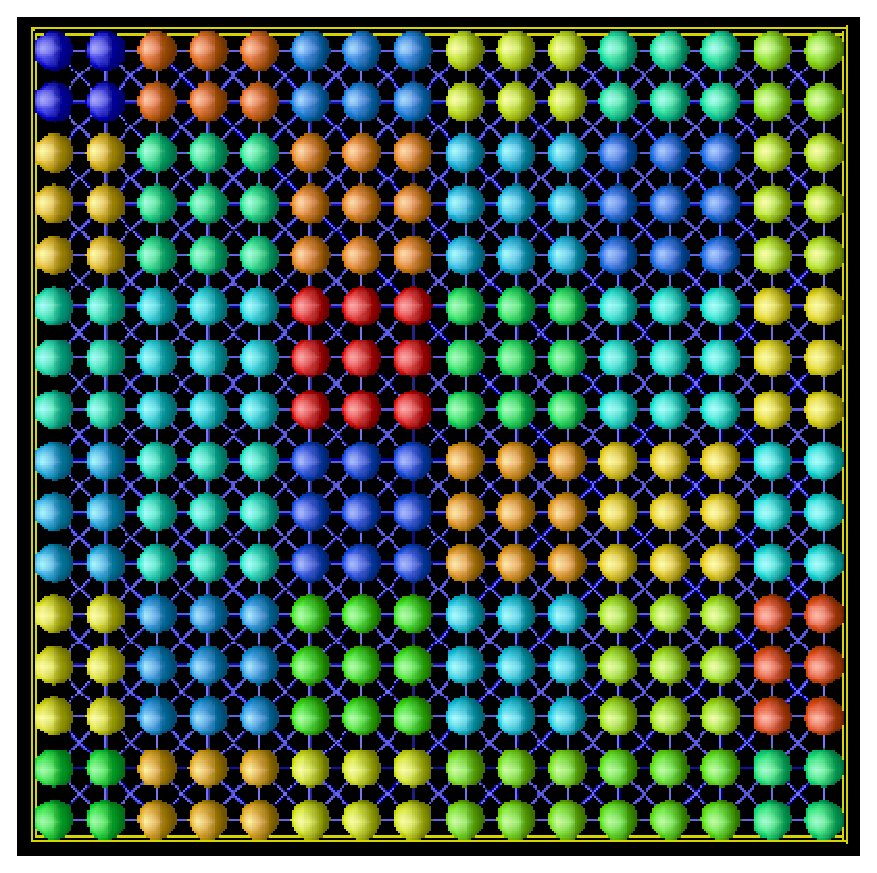
\includegraphics[height=6cm]{ml_Uncoupled-16x16.ps} \hspace{0.5cm}
  %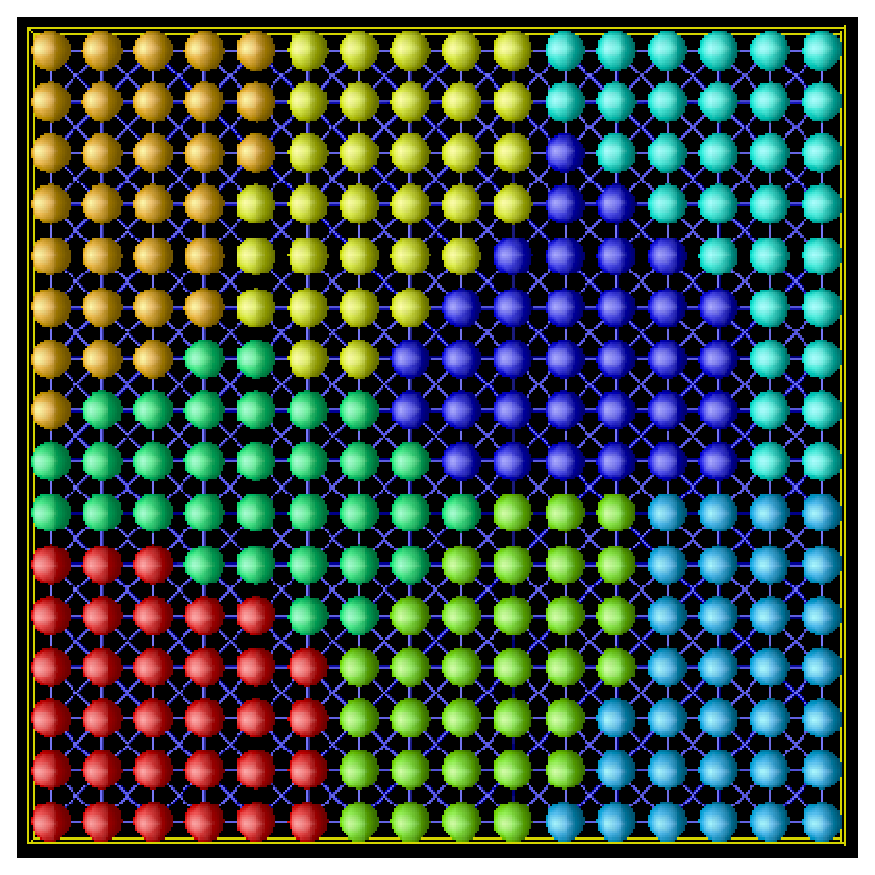
\includegraphics[height=6cm]{ml_METIS-16x16.ps}
  %\caption{Aggregates for Uncoupled (left) and METIS (right) for a 16x16 Cartesian grid.}
  %\label{fig:ml:comparison}
%\end{figure}

\begin{table}
\begin{center}
\begin{tabular}{ | p{5cm} | p{10cm} | }
\hline
\verb!Uncoupled! & For a $1$,$2$,or $3$ dimensional structured Cartesian grid 
                   with a $3$, $9$ or $27$ point stencil respectively,
                   construct aggregates of optimal size such that
                   each aggregate resides on one processor.\\
\verb!MIS! & Maximal independent set based coarsening with aggregates
             allowed to reside on multiple processes. 
             The scheme minimizes the number of iterations,
             but the cost per iteration is high.  \\
\verb!METIS! & Use a serial graph partitioner to create
               aggregates residing on one processor. 
               The number of nodes in each aggregate
               is specified with the option {\tt aggregation: nodes per aggregate}.
               ML must be configured with {\tt --with-ml\_metis}. \\
\verb!ParMETIS! & Use a parallel graph partitioner to create aggregates that
                  may reside on multiple processors.  
                  ML must be configured with {\tt --with-ml\_parmetis3x}. 
                  The number of aggregates is
                  specified by option {\tt aggregation: global number}. \\
\hline
\end{tabular}
\caption{ML\_Epetra::MultiLevelPreconditioner Coarsening Schemes}
\label{tab:ml:aggr}
\end{center}
\end{table}

\begin{table}
\begin{center}
\begin{tabular}{ | p{5cm} | p{10cm} | }
\hline
\verb!Jacobi! & Point-Jacobi. Damping factor is specified using
{\tt smoother: damping factor}, and the number of sweeps with {\tt
  smoother: sweeps} \\ 
\verb!Gauss-Seidel! & Point Gauss-Seidel. \\
\verb!Aztec! & Use AztecOO's built-in preconditioning functions as
smoothers. Or, use approximate solutions with AztecOO as smoothers. 
The AztecOO vectors \verb!options! and {\tt params} can be set using
{\tt smoother: Aztec options} and {\tt smoother: Aztec params}. \\
\hline
\end{tabular}
\caption{ML\_Epetra::MultiLevelPreconditioner Smoothers} 
\label{tab:ml:smoother}
\end{center}
\end{table}

\begin{table}
\begin{center}
\begin{tabular}{ | p{5cm} | p{10cm} | }
\hline
\verb!Jacobi! & Use Jacobi as a solver. \\
\verb!Gauss-Seidel! & Use Gauss-Seidel as a solver. \\
\verb!Amesos_KLU! & Use Amesos's KLU sequential solver. \\
\verb!Amesos_UMFPACK! & Use UMFPACK. \\
\verb!Amesos_Superludist! & Use SuperLU\_DIST. \\
\verb!Amesos_MUMPS! & Use MUMPS. \\
\hline
\end{tabular}
\caption{ML\_Epetra::MultiLevelPreconditioner Coarsest Grid Exact Solvers
  To use Amesos, ML must be configured with {\tt --enable-amesos} 
  and Amesos also be configured as needed.}
\label{tab:ml:coarse}
\end{center}
\end{table}

A very simple fragment of code using this class is reported below.
The reader may refer to file
\verb!$ML_HOME/examples/ml_example_MultiLevelPreconditioner.cpp! for a more
complex example. To run example, first 
configure ML \verb!--enable-triutils!.
\begin{verbatim}
#include "ml_include.h"
#include "ml_MultiLevelPreconditioner.h"
#include "Teuchos_ParameterList.hpp"

...

  // A is an Epetra_RowMatrix derived class object
  // solver is an AztecOO object

  Teuchos::ParameterList MList;

  // default values for smoothed aggregation
  ML_Epetra::SetDefaults("SA",MLList);
  MLList.set("max levels",6);
  MLList.set("increasing or decreasing","decreasing");
  MLList.set("aggregation: type", "MIS");
  MLList.set("coarse: type","Amesos_KLU");
  
  ML_Epetra::MultiLevelPreconditioner * MLPrec = 
    new ML_Epetra::MultiLevelPreconditioner(A, MLList, true);

  solver.SetPrecOperator(MLPrec);
  solver.SetAztecOption(AZ_solver, AZ_gmres);
  solver.Iterate(Niters, 1e-12);

  ...

  delete MLPrec;
\end{verbatim}
The general procedure is as follows. First, the user defines a Teuchos
parameters' list. Second input parameters are set via method
\verb!set(ParameterName,ParameterValue)!, where \verb!ParameterName! is
a string defining the parameter, and \verb!ParameterValue! is the
specified parameter, that can be any C++ object or pointer.  This list
is passed to the constructor, together with a pointer to the matrix, and
a boolean flag.  If this flag is set to \verb!false!, the constructor
will not compute the multilevel hierarchy until when
{\tt MLPrec->ComputePrecon-}\newline {\tt ditioner()} is called. The hierarchy can be
destroyed using \verb!MLPrec->Destroy()!.  For instance, the user may
define a code like:
\begin{verbatim}
  // A is still not filled with numerical values
  ML_Epetra::MultiLevelPreconditioner * MLPrec = 
    new ML_Epetra::MultiLevelPreconditioner(A, MLList, false);
  
  // compute the elements of A
  ...
  // now compute the preconditioner
  MLPrec->ComputePreconditioner();

  // solve the linear system, and refill A
  ...
  MLPrec->Destroy(); // destroy previous preconditioner,
  MLPrec->ComputePreconditioner(); // and build a new one
\end{verbatim}
In this fragment of code, the user defines the ML preconditioner, but
does not create the preconditioner in the construction phase. This is of
particular interest, for example, when ML is used in conjunction with
nonlinear solvers (like NOX~\cite{NOX-home-page}).

We point out that the input parameter list is {\sl copied} in the
construction phase, hence later changes to \verb!MLList! will not affect
the preconditioner. Should one need to modify parameters in the
\verb!MLPrec!'s internally stored parameter list, proceed as
follows:
\begin{verbatim}
  ParameterList & List = MLPrec->GetList();
\end{verbatim}
and then directly modify \verb!List!.

\medskip

All ML options can have a common prefix, specified by the
user in the construction phase. For example, suppose that we require
\verb!ML: ! to be the prefix. The constructor will be
\begin{verbatim}
  MLLIst.set("ML: aggregation: type", "METIS");
  ML_Epetra::MultiLevelPreconditioner * MLPrec = 
  new ML_Epetra::MultiLevelPreconditioner(*A,  
                                          MLList, 
                                          true, 
                                          Prefix);
\end{verbatim}
where \verb!Prefix! is a char array containing \verb!ML: !.

Note that spaces are important: Do not include leading or trailing
spaces, and separate words by just one space! Misspelled parameters will
not be used, and can be detected calling method \verb!PrintUnused()!
{\sl after} the construction of the multilevel hierarchy. 

For a detailed list of all the parameters, we refer to the ML user's
guide.  Here, we report the most used parameters in
Tables~\ref{tab:ml:aggr}, \ref{tab:ml:smoother} and \ref{tab:ml:coarse}.


%%%
%%%
%%%


\section{Two-Level Domain Decomposition Preconditioners with ML}
\label{sec:ml_DD}

The idea of two level domain decomposition based on aggregation is to
use a graph partitioner to partition the local or global graph into
subgraphs, and then treat each subgraph as a large aggregate.

The example contained herein 
uses the graph decomposition library METIS to create the coarse-level matrix.
If you don't have METIS, or just do not want to
re-configure ML, you may run the example 
you will be limited to use only one aggregate per process.
There are three changes to the Trilinos configuration.
One flag tells the package (ML) to look for an external library,
and the other two flag tells the compiler
where to find the include directories and external library.
Configure ML with the flags \verb!--with-ml_metis!,
and with {\tt --with-incdirs} and {\tt --with-ldflags}
set to the locations of the METIS include files and library. 
Please type {\tt configure --help} in the ML subdirectory for more information. 

Two-level domain decomposition methods are
effective for the iterative solution of many different kinds of linear
systems.  For some classes of problems, a very convenient way to define
the coarse grid operator is to use an aggregation procedure. This is very
close to what presented in Section~\ref{sec:ml_prec}. The main
difference is that only two level methods are considered, and that the
coarse grid remains of (relatively) small size. The idea is to define a
small number of aggregates on each process, using a graph decomposition
algorithm (as implemented in the library METIS, for
instance)\footnote{Aggregation schemes based on ParMETIS are also
available. Please refer to the help of the ML {\tt configure} for more
details.}. This can be done as follows.

The linear system matrix \verb!A!, here coded as an
Epetra\_CrsMatrix\footnote{Epetra\_VbrMatrix and Epetra\_RowMatrix can
  be used as well.}, corresponds to the descretization of a 2D Laplacian
on a Cartesian grid. \verb!x! and \verb!b! are the solution vector and
the right-hand side, respectively.

The AztecOO linear problem is defined as
\begin{verbatim}
  Epetra_LinearProblem problem(&A, &x, &b);
  AztecOO solver(problem);
\end{verbatim}

At this point, we can create the Teuchos parameters' list, with the
following parameters:
\begin{verbatim}
  ParameterList MLList;

  ML_Epetra::SetDefaults("DD",MLList);

  MLList.set("max levels",2);
  MLList.set("increasing or decreasing","increasing");

  MLList.set("aggregation: type", "METIS");
  MLList.set("aggregation: nodes per aggregate", 16);
  MLList.set("smoother: pre or post", "both");
  MLList.set("coarse: type","Amesos_KLU");
  MLList.set("smoother: type", "Aztec");
\end{verbatim}
The last option tells ML to use the Aztec preconditioning function as a
smoother. Aztec requires an integer vector \verb!options! and a double
vector \verb!params!. Those can be defined as follows:
\begin{verbatim}
  Teuchos::RCP<vector<int>> options = rcp(new vector<int>(AZ_OPTIONS_SIZE));
  Teuchos::RCP<vector<double>> params = rcp(new vector<double>(AZ_PARAMS_SIZE));
  AZ_defaults(options,params);
  AZ_defaults(&(*options)[0],&(*params)[0]);
  (*options)[AZ_precond] = AZ_dom_decomp;
  (*options)[AZ_subdomain_solve] = AZ_icc;

  MLList.set("smoother: Aztec options", options);
  MLList.set("smoother: Aztec params", params);
\end{verbatim}
The last two commands set the Teuchos reference-counted pointers,
{\tt options} and {\tt params}, in the parameter list.
Note that {\sl all} Aztec preconditioners can be used as smoothers for
ML. 
At this point we can create the ML preconditioner as
\begin{verbatim}
  ML_Epetra::MultiLevelPreconditioner * MLPrec =
    new ML_Epetra::MultiLevelPreconditioner(A, MLList, true);
\end{verbatim}
and check that no options have been misspelled, using
\begin{verbatim}
  MLPrec->PrintUnused();
\end{verbatim}
AztecOO solver is called using
\begin{verbatim}
  solver.SetPrecOperator(MLPrec);

  solver.SetAztecOption(AZ_solver, AZ_cg_condnum);

  int Niters = 500;
  solver.SetAztecOption(AZ_kspace, 160);

  solver.Iterate(Niters, 1e-12);
\end{verbatim}
Finally, some (limited) information about the preconditioning phase are
obtained using
\begin{verbatim}
  cout << MLPrec->GetOutputList();
\end{verbatim}
The entire code is reported in 
\newline
\TriExe{ml/ex2.cpp}.
\newline


\clearpage
\newpage
% @HEADER
% ***********************************************************************
% 
%            Trilinos: An Object-Oriented Solver Framework
%                 Copyright (2001) Sandia Corporation
% 
% Under terms of Contract DE-AC04-94AL85000, there is a non-exclusive
% license for use of this work by or on behalf of the U.S. Government.
% 
% This library is free software; you can redistribute it and/or modify
% it under the terms of the GNU Lesser General Public License as
% published by the Free Software Foundation; either version 2.1 of the
% License, or (at your option) any later version.
%  
% This library is distributed in the hope that it will be useful, but
% WITHOUT ANY WARRANTY; without even the implied warranty of
% MERCHANTABILITY or FITNESS FOR A PARTICULAR PURPOSE.  See the GNU
% Lesser General Public License for more details.
%  
% You should have received a copy of the GNU Lesser General Public
% License along with this library; if not, write to the Free Software
% Foundation, Inc., 51 Franklin St, Fifth Floor, Boston, MA 02110-1301
% USA
% Questions? Contact Michael A. Heroux (maherou@sandia.gov) 
% 
% ***********************************************************************
% @HEADER

\chapter{Interfacing Direct Solvers with Amesos}
\label{chap:amesos}

\ChapterAuthors{Marzio Sala}

\begin{introchapter}
The Amesos package provides an object-oriented interface to several
direct sparse solvers. Amesos will solve (using a direct factorization
method) the linear systems of equations (\ref{eq:linear_sys}) where $A$
is stored as an Epetra\_RowMatrix object, and $X$ and $B$ are
Epetra\_MultiVector objects.

The Amesos package has been designed to face some of the challenges of
direct solution of linear systems. In fact, many solvers have been
proposed in the last years, and often each of them requires different
input formats for the linear system matrix. Moreover, it is not uncommon
that the interface changes between revisions. Amesos aims to solve those
problems, furnishing a clean, consistent interface to many direct
solvers.
\end{introchapter}

\section{Introduction to the Amesos Design}

Using Amesos, users can interface their codes with a (large) variety of
direct linear solvers, sequential or parallel, simply by a code
instruction of type
\begin{verbatim}
AmesosProblem.Solver();
\end{verbatim}
Amesos will take care of redistributing data among the processors, if
necessary.


All the Amesos classes are derived from a base class mode,
\verb!Amesos_BaseSolver!. This abstract interface provides the basic
functionalities for all Amesos solvers, and allows users to choose
different direct solvers very easily -- by changing an input scalar
parameter. See Section~\ref{sec:amesos_generic} for more details.

In this Chapter, we will suppose that matrix $A$ in
equation~(\ref{eq:linear_sys}) is defined as an Epetra\_RowMatrix, in
principle with nonzero entries on all the processes defined in the
Epetra\_Comm communicator in use. $X$ and $B$, instead, are
Epetra\_MultiVector, defined on the same communicator.  

Amesos contains several classes: 
\begin{itemize}
\item \verb!Amesos_Lapack!: Interface to serial dense solver LAPACK.
\item \verb!Amesos_KLU!: Interface to Amesos's internal solver KLU. KLU
  is a serial, unblocked code ideal for getting started, and for very
  sparse matrices, such as circuit matrices. 
\item \verb!Amesos_Umfpack!: Interface to Tim Davis's
  UMFPACK~\cite{umfpack}. UMFPACK is a serial solver.
%\item \verb!Amesos_Dscpack!: Interface to Padma Raghavan's
%  DSCPACK~\cite{dscpack-home-page};
\item \verb!Amesos_Superludist!: Interface to Xiaoye S.~Li's SuperLU
  solver suite, including SuperLU, SuperLU\_DIST 1.0 and SuperLU\_DIST
  2.0~\cite{superlu-home-page}. SuperLU is a serial solvers, while
  SuperLU\_DIST is a parallel solver.
\item \verb!Amesos_Mumps!: Interface to MUMPS
  4.3.1~\cite{mumps-home-page}\footnote{At present, MUMPS is the only
    Amesos class that can take advantage of the symmetry of the linear
    system matrix.}. MUMPS is a parallel direct solver;
\item \verb!Amesos_Scalapack!: Interface to ScaLAPACK~\cite{scalapack},
  the parallel version of LAPACK\footnote{Note that Amesos does {\sl
      not} contain interfaces to LAPACK routines.  Other Trilinos
    packages already offer those routines (Epetra and Teuchos).  }.
\end{itemize}

If the supported packages is serial, and one is solving with more than
one process, matrix and right-hand side are shipped to process 0,
solved, then the solution is broadcasted to the distributed solution
vector $X$. For parallel solvers, instead, various options are
supported, depending on the package at hand:
\begin{itemize}
\item The Amesos\_Superludist interface can be used over all the
  processes, as well as on a subset of them. The matrix is kept in
  distributed form over the processes of interest;
\item Amesos\_Mumps can keep the matrix in a distributed form over all
  the processes, or the matrix can be shipped to processor 0. In both
  cases, all the processes in the MPI communicator will be used.
\end{itemize}

This Chapter, we will cover:
\begin{itemize}
\item The Amesos\_BaseSolver interface to various direct solvers,
  presented (in Section~\ref{sec:amesos_generic}).
\end{itemize}

%%%
%%%
%%%

\section{Amesos\_BaseSolver: A Generic Interface to Direct Solvers}
\label{sec:amesos_generic}

All Amesos objects are constructed from the function class
\verb!Amesos!.  Amesos allows a code to delay the
decision about which concrete class to use to implement the
Amesos\_BaseSolver interface. The main goal of this class is to allow
the user to select any supported (and enabled at configuration time)
direct solver, simply changing an input parameter. Another remarkable
advantage of Amesos\_BaseSolver is that, using this class, users does
not have to include the header files of the 3-part libraries in their
code\footnote{Using Amesos\_BaseSolver, 3-part libraries header files
  are required in the compilation of Amesos only.}.

An example of use of this class is as follows. First, the following
header files must be included:
\begin{verbatim}
  #include "Amesos.h" 
  #include "AmesosClassType.h"
\end{verbatim}
Then, let \verb!A! be an Epetra\_RowMatrix object (for instance, and
Epetra\_CrsMatrix). We need to define a linear problem,
\begin{verbatim}
  Epetra_LinearProblem * Amesos_LinearProblem = 
                         new Epetra_LinearProblem;
  Amesos_LinearProblem->SetOperator( A ) ; 
\end{verbatim}
and to create an Amesos parameter list (which can be empty):
\begin{verbatim}
  Teuchos::ParameterList ParamList ;
\end{verbatim}
Now, let \verb!Choice! be an string, with one of the
following values: 
\begin{itemize}
\item {\tt AMesos\_Klu};
\item {\tt Amesos\_Umfpack};
\item {\tt Amesos\_Mumps};
\item {\tt Amesos\_Superludist};
\item {\tt Amesos\_Scalapack}.
\end{itemize}
We can construct an \verb!Amesos_BaseSolver! object as follows:
\begin{verbatim}
  Amesos_BaseSolver * A_Base;
  Amesos A_Factory;

  A_Base = A_Factory.Create(Choice, *Amesos_LinearProblem, 
                            ParamList );
  assert(A_Base!=0);
\end{verbatim}
Symbolic and numeric factorizations are computed using methods
\begin{verbatim}
  A_Base->SymbolicFactorization();
  A_Base->NumericFactorization();
\end{verbatim}
The numeric factorization phase will check whether a symbolic
factorization exists or not. If not, method
\verb!SymbolicFactorization()! is invoked.  Solution is computed (after
setting of LHS and RHS in the linear problem), using
\begin{verbatim}
  A_Base->Solve();
\end{verbatim}
The solution phase will check whether a numeric factorization exists or
not. If not, method \verb!SymbolicFactorization()! is called.

Users must provide the nonzero structure of the matrix for the symbolic
phase, and the actual nonzero values for the numeric
factorization. Right-hand side and solution vectors must be set before
the solution phase, for instance using
\begin{verbatim}
  Amesos_LinearProblem->SetLHS(x);
  Amesos_LinearProblem->SetRHS(b);
\end{verbatim}

A common ingredient to all the Amesos classes is the Teuchos parameters'
list. This object, whose definition requires the input file
\verb!Teuchos_ParameterList.hpp!, is used to specify the parameters that
affect the 3-part libraries. Here, we simply recall that the parameters'
list can be created as
\begin{verbatim}
  Teuchos::ParameterList AmesosList;
\end{verbatim}
and parameters can be set as
\begin{verbatim}
  AmesosList.set(ParameterName,ParameterValue);
\end{verbatim}
Here, \verb!ParameterName! is a string containing the parameter name,
and \verb!ParameterValue! is any valid C++ object that specifies the
parameter value (for instance, an integer, a pointer to an array or to
an object).

For a detailed list of parameters we refer to~\cite{Amesos-Reference-Guide}.


\clearpage
\newpage
%@HEADER
% ************************************************************************
% 
%          Trilinos: An Object-Oriented Solver Framework
%              Copyright (2001) Sandia Corporation
% 
% Under terms of Contract DE-AC04-94AL85000, there is a non-exclusive
% license for use of this work by or on behalf of the U.S. Government.
% 
% This program is free software; you can redistribute it and/or modify
% it under the terms of the GNU General Public License as published by
% the Free Software Foundation; either version 2, or (at your option)
% any later version.
%   
% This program is distributed in the hope that it will be useful, but
% WITHOUT ANY WARRANTY; without even the implied warranty of
% MERCHANTABILITY or FITNESS FOR A PARTICULAR PURPOSE.  See the GNU
% General Public License for more details.
%   
% You should have received a copy of the GNU General Public License
% along with this program; if not, write to the Free Software
% Foundation, Inc., 675 Mass Ave, Cambridge, MA 02139, USA.
% 
% Questions? Contact Michael A. Heroux (maherou@sandia.gov)
% 
% ************************************************************************
%@HEADER

\chapter{Eigenvalue and Eigenvector Computations with Anasazi}
\label{chap:anasazi}

\ChapterAuthors{Christopher Baker, Heidi Thornquist}

\begin{introchapter}
Two goals motivated the development of the Anasazi eigensolver package: interoperability
and extensibility. The intention of \emph{interoperability} is to ease the use of Anasazi
in a wide range of application environments. To this end, the algorithms written in Anasazi utilize an
abstract interface for operators and vectors, allowing the user to leverage existing
linear algebra libraries. The concept of \emph{extensibility} drives 
development of Anasazi to allow users to make efficient use of Anasazi codes while
simultaneously enabling them to easily develop their own code in the Anasazi framework.
This is encouraged by promoting code modularization and multiple levels of access to
solvers and their data.

In this Chapter, we outline the Anasazi eigensolver framework and motivate the design.
In particular, we present
\begin{itemize}
  \item the Anasazi operator/vector interface (Section~\ref{sec:anasazi:opvec});
  \item the Anasazi eigensolver framework (Section~\ref{sec:anasazi:solver_framework});
  \item a description of Anasazi classes (Section~\ref{sec:anasazi:classes});
  \item the interface to the Epetra linear algebra package (Section~\ref{sec:anasazi:epetra});
  \item an example using Anasazi for the solution of an eigenvalue problem (Section~\ref{sec:anasazi:example}).
\end{itemize}
\end{introchapter}

\section{The Anasazi Operator/Vector Interface}
%%%%%%%%%%%%%%%%%%%%%%%%%%%%%%%%%%%%%%%%%%%%%%%%%%%%%%
\label{sec:anasazi:opvec}

The Anasazi eigensolver package utilizes abstract interfaces for operators and
multivectors. The goals of this are to leverage existing linear algebra libraries and to
protect previous software investment. Algorithms in Anasazi are developed at a high-level,
where the underlying linear algebra objects are opaque. The choice in linear algebra is
made through templating, and access to the functionality of the underlying objects is
provided via the traits classes Anasazi::MultiVecTraits and Anasazi::OperatorTraits.

These classes define opaque interfaces, specifying the operations that multivector and
operator classes must support in order to be used in Anasazi without exposing low-level
details of the underlying data structures.

The benefit of using a templated traits class over inheritance is that the latter requires
the user to derive multivectors and operators from Anasazi-defined abstract
base classes. The former, however, defines only local requirements: Anasazi-defined traits
classes implemented as user-developed adapters for the chosen multivector and operator
classes.

Anasazi::MultiVecTraits provides routines for the creation of multivectors, as well as
their manipulation. In order to use a specific scalar type and multivector type with
Anasazi, there must exist a template specialization of Anasazi::MultiVecTraits for this
pair of classes. A full list of methods required by Anasazi::MultiVecTraits is given in
Table~\ref{tab:anasazi:mvt}.

\begin{table}
\begin{center}
\begin{tabular}{| p{4cm} || p{8cm} |}
\hline
Method name & Description \\
\hline\hline
Clone           & Creates a new empty multivector containing a specified number of columns.  \\\hline
CloneCopy       & Creates a new multivector with a copy of the contents of an existing multivector (deep copy). \\\hline
CloneView       & Creates a new multivector that shares the selected contents of an existing multivector (shallow copy).  \\\hline
GetVecLength    & Returns the vector length of a multivector.  \\\hline
GetNumberVecs   & Returns the number of vectors in a multivector.  \\\hline
MvTimesMatAddMv & Apply a SerialDenseMatrix $M$ to another multivector $A$, $B \leftarrow \alpha A M + \beta B$.  \\\hline
MvAddMv         & Perform $mv \leftarrow \alpha A + \beta B$.  \\\hline
MvTransMv       & Compute the matrix $C \leftarrow \alpha A^H B$.  \\\hline
MvDot           & Compute the vector $b$ where the components are the individual dot-products of the $i$-th columns of $A$ and $B$, i.e. $b[i] = A[i]^H B[i]$.  \\\hline
MvScale         & Scale the columns of a multivector. \\\hline
MvNorm          & Compute the 2-norm of each individual vector of $A$.  \\\hline
SetBlock        & Copy the vectors in $A$ to a subset of vectors in $B$. \\\hline
MvRandom        & Replace the vectors in $A$ with random vectors.  \\\hline
MvInit          & Replace each element of the vectors in $A$ with $\alpha$.  \\\hline
MvPrint         & Print the multi-vector to an output stream.  \\\hline
\hline
\end{tabular}
\caption{Methods required by MultiVecTraits interface.}
\label{tab:anasazi:mvt}
\end{center}
\end{table}

Just as Anasazi::MultiVecTraits defined the interface required to use a
multivector class with Anasazi, Anasazi::OperatorTraits defines the
interface required to use the combination of a specific operator class with a
specific multivector class. This interface defines a single method:
\begin{verbatim}
OperatorTraits<ScalarType,MV,OP>::Apply(const OP &Op, const MV &x, MV &y)
\end{verbatim}
This method performs the operation $y = Op(x)$, where $Op$ is an operator of type
\verb!OP! and $x$ and $y$ are multivectors of type \verb!MV!. In order to use the
combination of \verb!OP! and \verb!MV!, there must be a specialization of
Anasazi::OperatorTraits for \verb!ScalarType!, \verb!OP! and \verb!MV!. 

Calling methods of MultiVecTraits and OperatorTraits requires that specializations of
these traits classes have been implemented for given template arguments.  
Anasazi provides the following specializations of these traits classes:
\begin{itemize}
  \item Epetra\_MultiVector and Epetra\_Operator (with scalar type double)    
  \item Thyra::MultiVectorBase and Thyra::LinearOpBase (with arbitrary scalar type) \\
        This allows Anasazi to be used with any classes that implement the abstract interfaces provided by the Thyra package.    
  \item Anasazi::MultiVec and Anasazi::Operator (with arbitrary scalar type) \\
        This allows Anasazi to be used with any classes that implement the abstract base
        classes Anasazi::MultiVec and Anasazi::Operator.
\end{itemize}

For user-specified classes that don't match one of the above, specializations of
MultiVecTraits and OperatorTraits will need to be created by the user for use by Anasazi.
Test routines \verb!Anasazi::TestMultiVecTraits()! and
\verb!Anasazi::TestOperatorTraits()! are provided by Anasazi to help in testing
user-developed adapters.


\section{The Anasazi Eigensolver Framework}
%%%%%%%%%%%%%%%%%%%%%%%%%%%%%%%%%%%%%%%%%%%%%%%%%%%%%%
\label{sec:anasazi:solver_framework}

The goals of flexibility and efficiency can interfere with the goals of simplicity and
ease of use. For example, efficient memory use and low-level data access required in
scientific codes can lead to complicated interfaces and violations of standard
object-oriented development practices.

In Anasazi, this problem is addressed by providing a multi-tiered access strategy for
eigensolver algorithms. Anasazi users have the choice of interfacing at one of two levels:
either working at a high-level with a eigensolver manager or working at a low-level
directly with an eigensolver.

Consider as an example the block Davidson iteration. The essence of this iteration can be
distilled into the following algorithm:
\begin{enumerate}
  \item apply preconditioner $N$ to the current residuals: $H = N R$
  \item use $H$ to expand current basis $V$
  \item use new $V$ to compute a projected eigenproblem
  \item solve the projected eigenproblem and form the Ritz vectors $X$ and Ritz values
    $\Theta$ 
  \item compute the new residuals $R$
\end{enumerate}

In implementing a block Davidson method, this iteration repeats until the basis $V$ is full
(in which case it is time to restart) or some stopping criterion has been satisfied. Many
valid stopping criteria exist, as well as many different methods for restarting the basis.
Both of these, however, are distinct from the essential iteration as described above. A
user wanting to perform block Davidson iterations could ask the solver to perform these
iterations until a user-specified stopping criterion was satisfied or the basis was full,
at which time the user would perform a restart. This allows the user complete control over
the stopping criteria and the restarting mechanism, and leaves the eigensolver responsible
for a relatively simple bit of state and behavior.

This is the way that Anasazi has been designed. The eigensolvers (encapsulating an
iteration and the associated state) are derived classes of the abstract base class
Anasazi::Eigensolver. The goals of this class are three-fold:
\begin{itemize}
  \item to define an interface used for checking the status of a solver by a status test;
  \item to contain the essential iteration associated with a particular eigensolver iteration;
  \item to contain the state associated with that iteration.
\end{itemize}

The status tests, assembled to describe a specific stopping criterion and queried by the eigensolver
during the iteration, are represented as subclasses of Anasazi::StatusTest. The
communication between status test and eigensolver occurs
inside of the \verb!iterate()! method provided by each Anasazi::Eigensolver. This code
generally takes the form:
\begin{verbatim}
SomeEigensolver::iterate() {
  while ( statustest.checkStatus(this) != Passed ) {
    //
    // perform eigensolver iterations
    //
  }
  return;  // return back to caller
}
\end{verbatim}

Each Anasazi::StatusTest provides a method, \verb!checkStatus()!, which through queries to
the methods provided by Anasazi::Eigensolver, determines whether the solver meets the
criteria defined by that particular status test. After a solver returns from
\verb!iterate()!, the caller has the option of accessing the state associated with the
solver and re-initializing the solver with a new state.

While this method of interfacing with the solver is powerful, it can be tedious.
This method requires that user construct a number of support classes, in addition to
managing call to \verb!Eigensolver::iterate()!.
The Anasazi::SolverManager class was developed to
address this complaint. A solver manager is a class that wraps around an eigensolver,
providing additional functionality while also handling lower-level interaction with the
eigensolver that a user may not wish to handle. Solver managers are intended to be 
easy to use, while still providing the features and flexibility needed to solve real-world
eigenvalue problems. For example, the Anasazi::BlockDavidsonSolMgr takes only two
arguments in its constructor: an Anasazi::Eigenproblem specifying the eigenvalue problem
to be solved and a Teuchos::ParameterList of options specific to this solver manager. The
solver manager instantiates an eigensolver, along with the status tests and other support
classes needed by the eigensolver. To solve the eigenvalue problem, the user simply calls
the \verb!solve()! method of the solver manager. The solver manager performs repeated
calls to the eigensolver \verb!iterate()! method, performs restarts and locking, and
places the final solution into the eigenproblem.

Users therefore have a number of options for performing eigenvalue computations with Anasazi:
\begin{itemize}
  \item use an existing solver manager;\\
        In this case, the user is limited to the functionality provided by the current eigensolvers.
  \item develop a new solver manager around an existing eigensolver;\\
        The user can extend the functionality provided by the eigensolver, specifying 
        custom configurations for status tests, orthogonalization, restarting, locking,
        etc.
  \item develop a new eigensolver/solver manager;\\
        The user can write an eigensolver for an iteration that is not represented in
        Anasazi. The user still has the benefit of the support classes provided by 
        Anasazi, and the knowledge that the new solver/solver manager can be easily
        used by anyone already familiar with Anasazi.
\end{itemize}


\section{Anasazi Classes}
%%%%%%%%%%%%%%%%%%%%%%%%%%%%%%%%%%%%%%%%%%%%%%%%%%%%%%
\label{sec:anasazi:classes}

Anasazi is designed with extensibility in mind, so that users can augment the package with
any special functionality that they need. However, the released version of Anasazi
provides all functionality necessary for solving a wide variety of problems. This section
list and briefly describes the current classes found in Anasazi.

The solution of an eigenvalue problem requires a minimum subset of Anasazi classes. The
following is a list of classes that any Anasazi user must be familiar with to use the
package.

\begin{remark}
Anasazi makes extensive use of the Teuchos utility classes, especially
Teuchos::RCP (Section~\ref{sec:teuchos:RCP}) and
Teuchos::ParameterList (Section~\ref{sec:teuchos:ParameterList}). Users
are encouraged to become familiar with these classes and their correct
usage.
\end{remark}

\subsection{Anasazi::Eigenproblem}
%%%%%%%%%%%%%%%%%%%%%%%%%%%
\label{sec:anasazi:eigenproblem}

Anasazi::Eigenproblem is a container for the components of an eigenvalue problem, as well
as the solutions. By requiring eigenproblems to derive from Anasazi::Eigenproblem, Anasazi
defines a minimum interface that can be expected of all eigenvalue problems by the classes
that will work with the problems (e.g., eigensolvers and status testers).

Both the eigenproblem and the eigensolver in Anasazi are templated 
on the scalar type, the multivector type and the operator type. Before
declaring an eigenproblem, users must choose classes to represent these
entities. Having done so, they can begin to specify the parameters of the
eigenvalue problem. The Anasazi::Eigenproblem defines \textbf{set} methods for
the parameters of the eigenproblem. These methods are:
\begin{itemize}
\item \verb!setOperator! - set the operator for which the eigenvalues will be computed
\item \verb!setA! - set the $A$ operator for the eigenvalue problem $A x = M x \lambda$
\item \verb!setM! - set the $M$ operator for the eigenvalue problem $A x = M x \lambda$
\item \verb!setPrec! - set the preconditioner for the eigenvalue problem
\item \verb!setInitVec! - set the initial iterate
\item \verb!setAuxVecs! - set the auxiliary vectors, a subspace used to constrain the
  search space for the solution
\item \verb!setNEV! - set the number of eigenvalues to be computed
\item \verb!setHermitian! - specify whether the problem is Hermitian
\end{itemize}
In addition to these \textbf{set} methods, Anasazi::Eigenproblem defines
a method \verb!setProblem()! that gives the class the opportunity to perform
any initialization that may be necessary before the problem is handed off to an
eigensolver, in addition to verifying that the problem has been adequately defined. 

For each of the \textbf{set} methods listed above, there is a corresponding
\textbf{get} function. These are the functions used by eigensolvers and solver managers to get
the necessary information from the eigenvalue problem. In addition, there are
two methods for storing and retrieving the results of the eigenvalue computation:
\begin{verbatim}
const Eigensolution & getSolution();
void                  setSolution(const Eigensolution & sol);
\end{verbatim}
The Anasazi::Eigensolution structure is described in
Section~\ref{sec:anasazi:eigensolution}.

Anasazi provides users with a basic implementation of
Anasazi::Eigenproblem, called Anasazi::BasicEigenproblem
(Section~\ref{sec:anasazi:example}).
This formulation provides all the functionality
necessary to describe both generalized and standard linear eigenvalue problems.


\subsection{Anasazi::Eigensolution}
%%%%%%%%%%%%%%%%%%%%%%%%%%%
\label{sec:anasazi:eigensolution}

The Anasazi::Eigensolution structure was developed in order to facilitate setting
and retrieving of solution data. The class contains the following information:
\begin{itemize}
  \item \verb!Teuchos::RCP< MV > Evecs! \\ 
   The computed eigenvectors.
 \item \verb!Teuchos::RCP< MV > Espace! \\ 
   An orthonormal basis for the computed eigenspace.
 \item \verb!std::vector< Value< ScalarType > > Evals! \\ 
   The computed eigenvalues.
 \item \verb!std::vector< int > index! \\ 
   An index into \verb!Evecs! to enable compressed storage of eigenvectors for real, non-Hermitian problems.
 \item \verb!int numVecs! \\
   The number of computed eigenpairs.
\end{itemize}

All Anasazi solver managers place the results of the computation in the
Anasazi::Eigen\-problem class using an Anasazi::Eigensolution structure. The number of
eigensolutions computed is given by field \verb!numVecs!. The eigenvalues are
always stored as two real values, even when templated on a complex data type or when the eigenvalues
are real. Similarly, the eigenspace can always be represented by a multivector of width
\verb!numVecs!, even for non-symmetric eigenproblems over the real field. The storage
scheme for eigenvectors requires more finesse.

When solving real symmetric eigenproblems, the eigenvectors can always be chosen to be
real, and therefore can be stored in a single column of a real multivector. When solving
eigenproblems over a complex field, whether Hermitian or non-Hermitian, the eigenvectors
may be complex, but the multivector is defined over the complex field, so that this poses
no problem. However, real non-symmetric problems can have complex eigenvectors, which
prohibits a one-for-one storage scheme using a real multivector.  Fortunately, the
eigenvectors in this scenario occur as complex conjugate pairs, so the pair can be stored
in two real vectors. This permits a compressed storage scheme, which uses an index vector
stored in the Eigensolution, allowing conjugate pair eigenvectors to be easily retrieved
from \verb!Evecs!. 

The integers in Anasazi::Eigensolution::index take one of three values: $\{0, +1, -1\}$.
These values allow the eigenvectors to be retrieved as follows:
\begin{itemize}
  \item $index[i]=0$: the $i$-th eigenvector is stored uncompressed in column $i$ of
    \verb!Evecs!.
  \item $index[i]=+1$: the $i$-th eigenvector is stored compressed, with the real
    component in column $i$ of \verb!Evecs! and the \emph{positive} complex component
    stored in column $i+1$ of \verb!Evecs!
  \item $index[i]=-1$: the $i$-th eigenvector is stored compressed, with the real
    component in column $i-1$ of \verb!Evecs! and the \emph{negative} complex component
    stored in column $i$ of \verb!Evecs!
\end{itemize}
Because this storage scheme is only required for non-symmetric problems over the real
field, all other eigenproblems will result in an index vector composed entirely of zeroes.
For the real non-symmetric case, the $+1$ index will always immediately precede the
corresponding $-1$ index.

\begin{remark}
  Solver managers all put the computed eigensolution into the eigenproblem class before
  returning from \verb!solve()!. Eigensolvers do not; a user working directly with an
  eigensolver will need to recover the solution directly from the eigensolver state.
\end{remark}

\subsection{Anasazi::Eigensolver}
%%%%%%%%%%%%%%%%%%%%%%%%%%%
\label{sec:anasazi:eigensolver}

The Anasazi::Eigensolver class defines the basic interface that must be
met by any eigensolver class in Anasazi. The specific eigensolvers are
implemented as derived classes of Anasazi::Eigensolver.
Table~\ref{tab:anasazi:solvers} lists the eigensolver currently implemented in
Anasazi.

\begin{table}[htp]
\begin{center}
\begin{tabular}{| p{4cm} p{10cm} |}
\hline
Solver & Description \\
\hline
{\tt BlockDavidson}    & A block Davidson solver for Hermitian
                         eigenvalue problems.\\
{\tt BlockKrylovSchur} & A block Krylov Schur solver for Hermitian or
                         non-Hermitian eigenvalue problems.\\
{\tt LOBPCG} & The locally optimal block preconditioned conjugate gradient
method for Hermitian eigenproblems.\\
\hline
\end{tabular}
\caption{Eigensolvers currently implemented in Anasazi.}
\label{tab:anasazi:solvers}
\end{center}
\end{table}

Each eigensolver provides two significant types of methods: status methods and
solver-specific state methods. The status methods are defined by the Anasazi::Eigensolver
abstract base class and represent the information that a generic status test can request
from any eigensolver. A list of these methods is given in
Table~\ref{tab:anasazi:genstatusmethods}.

\begin{table}[htp]
\begin{center}
\begin{tabular}{| p{4cm} p{10cm} |}
\hline
Method & Description \\
\hline
{\tt getNumIters}       & Get the current number of iterations. \\
{\tt getRitzValues}     & Get the most recent Ritz values. \\
{\tt getRitzVectors}    & Get the most recent Ritz vectors. \\
{\tt getRitzIndex}      & Get the Ritz index needed for indexing compressed Ritz vectors. \\
{\tt getResNorms}       & Get the most recent residual norms, with respect to the OrthoManager. \\
{\tt getRes2Norms}      & Get the most recent residual 2-norms. \\
{\tt getRitzRes2Norms}  & Get the most recent Ritz residual 2-norms. \\
{\tt getCurSubspaceDim} & Get the current subspace dimension. \\
{\tt getMaxSubspaceDim} & Get the maximum subspace dimension. \\
{\tt getBlockSize}      & Get the block size. \\
\hline
\end{tabular}
\caption{A list of generic status methods provided by Anasazi::Eigensolver.}
\label{tab:anasazi:genstatusmethods}
\end{center}
\end{table}

The class Anasazi::Eigensolver, like Anasazi::Eigenproblem, is templated on the scalar
type, multivector type and operator type. The options for the eigensolver are passed
through the constructor, defined by Anasazi::Eigensolver to have the following form:
\begin{verbatim}
Eigensolver( 
   const Teuchos::RCP< Eigenproblem<ST,MV,OP> > &problem, 
   const Teuchos::RCP< SortManager<ST,MV,OP>  > &sorter,
   const Teuchos::RCP< OutputManager<ST>      > &printer,
   const Teuchos::RCP< StatusTest<ST,MV,OP>   > &tester,
   const Teuchos::RCP< OrthoManager<ST,OP>    > &ortho,
   ParameterList                                        &params  
 );
\end{verbatim}

These classes are used as follows:
\begin{itemize}
  \item \verb!problem! - the eigenproblem to be solved; the solver will
    get the problem operators from here.
  \item \verb!sorter! - the sort manager selects the significant eigenvalues; see
    Section~\ref{sec:anasazi:sorter}.
  \item \verb!printer! - the output manager dictates verbosity level in addition to 
    processing output streams; see Section~\ref{sec:anasazi:printer}.
  \item \verb!tester! - the status tester dictates when the solver should quit
    \verb!iterate()! and return to the caller; see Section~\ref{sec:anasazi:tester}.
  \item \verb!ortho! - the orthogonalization manager defines the inner product and other
    concepts related to 
    orthogonality, in addition to performing these computations for the solver; see
    Section~\ref{sec:anasazi:ortho}.
  \item \verb!params! - the parameter list specifies eigensolver-specific options; see the
    documentation for a list of options support by individual solvers.
\end{itemize}

In addition to specifying an iteration, an eigensolver also specifies a concept of state,
i.e. the current data associated with the iteration. After declaring an Eigensolver
object, the state of the solver is in an uninitialized state. For most solver, to be
initialized mean to be in a valid state, containing all of the information necessary for
performing eigensolver iterations. Anasazi::Eigensolver provides two methods concerning
initialization: \verb!isInitialized()! indicates whether the solver is initialized or not,
and \verb!initialize()! (with no arguments) instructs the solver to initialize itself
using random data or the initial vectors stored in the eigenvalue problem.

To ensure that solvers can be used as efficiently as possible, 
the user needs access to the state of the
solver. To this end, each eigensolver provides low-level methods for getting and setting the
state of the solver:
\begin{itemize}
  \item \verb!getState()! - returns a solver-specific structure with read-only pointers to
    the current state of the solver.
  \item \verb!initialize(...)! - accepts a solver-specific structure enabling the user to
    initialize the solver with a particular state.
\end{itemize}

The combination of these two methods, along with the flexibility provided by status tests,
allows the user almost total control over eigensolver iterations.


\subsection{Anasazi::SolverManager}
%%%%%%%%%%%%%%%%%%%%%%%%%%%
\label{sec:anasazi:solvermanager}

Using Anasazi by interfacing directly with eigensolvers is extremely powerful, but can be
tedious. Solver managers provide a way for users to encapsulate specific solving
strategies inside of an easy-to-use class. Novice users may prefer to use existing solver
managers, while advanced user may prefer to write custom solver managers.

Anasazi::SolverManager defines only two methods: a constructor accepting an
Anasazi::\-Eigenproblem and a parameter list of solver manager-specific options; and a
\verb!solve()! method, taking no arguments and returning 
either Anasazi::Converged or Anasazi::Unconverged.
Consider the following example code:
\begin{verbatim}
// create an eigenproblem
Teuchos::RCP< Anasazi::Eigenproblem<ScalarType,MV,OP> > problem = ...;
// create a parameter list
Teuchos::ParameterList params;
params.set(...);
// create a solver manager
Anasazi::BlockDavidsonSolMgr<ScalarType,MV,OP> solman(problem,params);
// solve the eigenvalue problem
Anasazi::ReturnType ret = solman.solve();
// get the solution from the problem
Anasazi::Eigensolution sol = problem->getSolution();
\end{verbatim}

\begin{remark}
  Errors in Anasazi are communicated via exceptions. This is outside the scope of this
  tutorial; see the Anasazi documentation for more information.
\end{remark}

As has been stated before, the goal of the solver manager is to create an eigensolver
object, along with the support objects needed by the eigensolver. Another purpose of many
solver managers is to manage and initiate the repeated calls to the underlying solver's
\verb!iterate()! method. For solvers that build a Krylov subspace to some maximum
dimension (e.g., BlockKrylovSchur and BlockDavidson), the solver manager will also assume
the task of restarting the solver when the subspace is full. This is something for which
multiple approaches are possible. Also, there may be substantial flexibility in creating
the support classes (e.g., sort manager, status tests) for the solver. An aggressive
solver manager could even go so far as to construct a preconditioner for the eigenvalue
problem. 

These examples are meant to illustrate the flexibility that specific solver managers may
have in implementing the \verb!solve()! routine. Some of these options might best be
incorporated into a single solver manager, which takes orders from the user via the
parameter list given in the constructor. Some of these options may better be contained in
multiple solver managers, for the sake of code simplicity. It is even possible to write
solver managers that contain other solvers managers; motivation for something like this
would be to select the optimal solver manager at runtime based on some expert knowledge,
or to create a hybrid method which uses the output from one solver manager to
initialize another one.

\subsection{Anasazi::StatusTest}
%%%%%%%%%%%%%%%%%%%%%%%%%%%
\label{sec:anasazi:tester}

By this point in the tutorial, the purpose of the Anasazi::StatusTest should be clear: to
give the user or solver manager flexibility in stopping the eigensolver iterations in
order to interact directly with the solver.

Many reasons exist for why a user would want to stop the solver from iterating:
\begin{itemize}
  \item some convergence criterion has been satisfied and it is time to quit;
  \item some part of the current solution has reached a sufficient accuracy to removed
    from the iteration (``locking'');
  \item the solver has performed a sufficient or excessive number of iterations.
\end{itemize}
These are just some commonly seen reasons for ceasing the iteration, and each of these can
be so varied in implementation/parametrization as to require some abstract mechanism
controlling the iteration.

The following is a list of Anasazi-provided status tests:
\begin{itemize}
  \item Anasazi::StatusTestCombo - this status test allows for the boolean combination of
    other status tests, creating near unlimited potential for complex status tests.
  \item Anasazi::StatusTestOutput - this status test acts as a wrapper around another
    status test, allowing for printing of status information on a call to
    \verb!checkStatus()!
  \item Anasazi::StatusTestMaxIters - this status test monitors the number of iterations
    performed by the solver; it can be used to halt the solver at some maximum number of iterations
    or even to require some minimum number of iterations.
  \item Anasazi::StatusTestResNorm - this status test monitors the residual norms of the
    current iterate.
  \item Anasazi::StatusTestOrderedResNorm - this status test also monitors the residual
    norms of the current iterate, but only considers the residuals associated with the
    most significant part of the current iterate.
\end{itemize}

\subsection{Anasazi::SortManager}
%%%%%%%%%%%%%%%%%%%%%%%%%%%
\label{sec:anasazi:sorter}

The purpose of a sort manager is to separate the eigensolver classes from the
sorting functionality required by those classes. This satisfies the flexibility
principle sought by Anasazi, by giving users the opportunity to perform the
sorting in whatever manner is deemed to be most appropriate. Anasazi defines an
abstract class Anasazi::SortManager with two methods, one for sorting real
values and one for sorting complex values:
\begin{verbatim}
ReturnType sort (..., std::vector<MagnitudeType> &evals, 
                      std::vector<int> *perm) 
ReturnType sort (..., std::vector<MagnitudeType> &r_evals, 
                      std::vector<MagnitudeType> &i_evals, 
                      std::vector<int> *perm)
\end{verbatim}
Each of these sort routines will sort the eigenvalues according to some
implementation and optionally return the permutation vector as well (useful for
sorting associated vectors). 

Anasazi provides a derived class Anasazi::BasicSort.  This class provides basic sorting
functionality, described in Table~\ref{tab:anasazi:sm}.

\begin{table}
\begin{center}
\begin{tabular}{| p{2cm} l |}
\hline
Option & Action \\
\hline
{\tt SM} & Sort eigenvalues in increasing order of magnitude \\
{\tt SR} & Sort eigenvalues in increasing order of real part \\
{\tt SI} & Sort eigenvalues in increasing order of imaginary part \\
{\tt LM} & Sort eigenvalues in decreasing order of magnitude \\
{\tt LR} & Sort eigenvalues in decreasing order of real part \\
{\tt LI} & Sort eigenvalues in decreasing order of imaginary part \\
\hline
\end{tabular}
\caption{Options for Anasazi::BasicSort.}
\label{tab:anasazi:sm}
\end{center}
\end{table}


\subsection{Anasazi::OrthoManager}
%%%%%%%%%%%%%%%%%%%%%%%%%%%
\label{sec:anasazi:ortho}

Orthogonalization and orthonormalization are commonly performed computations in iterative
eigensolvers; in fact, for some eigensolvers, they represent the dominant cost.  Different
scenarios may require different approaches (e.g., Euclidean inner product versus $M$ inner
product, orthogonal projections versus oblique projections).  Combined with the plethora
of available methods for performing these computations, Anasazi has left as much leeway to
the users as possible.

Orthogonalization of multivectors in Anasazi is performed by derived classes of
the abstract class Anasazi::OrthoManager. This class provides five methods:
\begin{itemize}
  \item \verb!innerProd(X,Y,Z)! - performs the inner product defined by the manager.
  \item \verb!norm(X)! - computes the norm induced by \verb!innerProd()!.
  \item \verb!project(X,C,Q)! - given an orthonormal basis $Q$, projects $X$ onto to the space perpindicular to
    $colspan(Q)$, optionally returning the coefficients of $X$ in $Q$.
  \item \verb!normalize(X,B)! - returns an orthonormal basis for $colspan(X)$, optionally
    returning the coefficients of $X$ in the computed basis.
  \item \verb!projectAndNormalize(X,C,B,Q)! - computes an orthonormal basis for subspace
    \newline
    $colspan(X) - colspan(Q)$, optionally returning the coefficients of
    $X$ in $Q$ and the new basis.
\end{itemize}

It should be noted that a call to \verb!projectAndNormalize()! is not necessarily
equivalent to a call to \verb!project()! followed by \verb!normalize()!. This follows from
the fact that, for some orthogonalization managers, a call to \verb!normalize()! may
augment the column span of a rank-deficient multivector in order to create an orthonormal
basis with the same number of columns as the input multivector. In this case, the code
\begin{verbatim}
orthoman.project(X,C,Q);
orthoman.normalize(X,B);
\end{verbatim}
\noindent could result in an orthonormal basis $X$ that is not orthogonal to the basis in $Q$.

Anasazi provides two orthogonalization managers:
\begin{itemize}
  \item Anasazi::BasicOrthoManager - performs orthogonalization using multiple steps of
    classical Gram-Schmidt.
  \item Anasazi::SVQBOrthoManager - performs orthogonalization using the SVQB
    orthogonalization technique described by Stathapoulos and Wu.
\end{itemize}

More information on these orthogonalization managers is available in the Anasazi
documentation.

\subsection{Anasazi::OutputManager}
%%%%%%%%%%%%%%%%%%%%%%%%%%%
\label{sec:anasazi:printer}

The output manager in Anasazi exists to provide
flexibility with regard to the verbosity of the eigensolver. Each output manager has
two primary concerns: what output is printed and where the output is printed to.
When working with the output manager, output is classified into one of the 
message types from Table~\ref{tab:anasazi:om}.

\begin{table}
\begin{center}
  \begin{tabular}{| p{4cm} p{8cm} |}
\hline
Message type & Description \\
\hline
{\tt Errors           } & Errors (always printed)  \\
{\tt Warnings         } & Warning messages   \\
{\tt IterationDetails } & Approximate eigenvalues, errors   \\
{\tt OrthoDetails     } & Orthogonalization/orthonormalization checking \\
{\tt FinalSummary     } & Final computational summary (usually from SolverManager::solve())  \\
{\tt TimingDetails    } & Timing details  \\
{\tt StatusTestDetails} & Status test details   \\
{\tt Debug            } & Debugging information \\
\hline
\end{tabular}
\caption{Message types used by Anasazi::OutputManager.}
\label{tab:anasazi:om}
\end{center}
\end{table}

Output manager in Anasazi are subclasses of the abstract base class
Anasazi::Output\-Manager. This class provides the following output-related methods:
\begin{itemize}
  \item {\tt bool isVerbosity (MsgType type)} - 
  Find out whether we need to print out information for this message type.
\item {\tt void  print (MsgType type, const string output)} - 
  Send output to the output manager.
\item {\tt ostream \& stream (MsgType type)} - 
  Create a stream for outputting to.
\end{itemize}

The output manager is meant to ease some of the difficulty associated with I/O in a
distributed programming environment. For example, consider some debugging output requiring
optional computation. For reasons of efficiency, we may want to perform the computation
only if debugging is requested; i.e., \verb!isVerbosity(Anasazi::Debug) == true!. However,
while we need all nodes to enter the code block to perform the computation, we probably
want only one of them to print the output. Furthermore, the user may want different types
of output treated in a different manner. The abstraction of the printing
mechanism allows both of these goals to be met.

Anasazi provides a single output manager, Anasazi::BasicOutputManager. This class accepts
an output stream from the user. The output corresponding to the verbosity level of the
manager is sent to this stream only on the master node; the output for other nodes is
neglected.

\section{Using the Anasazi adapter to Epetra}
%%%%%%%%%%%%%%%%%%%%%%%%%%%%%%%%%%%%%%%%%%%%%%%%%%%%%%
\label{sec:anasazi:epetra}

The Epetra package provides the underlying linear algebra foundation for many
Trilinos solvers.  By using the Anasazi adapter to Epetra, users not only
avoid the trouble of designing their own multivector and operator classes, but
they also gain the ability to utilize any other Trilinos package which
recognizes Epetra classes (such as AztecOO, IFPACK, and others).

In order to use the Anasazi adapter to Epetra, users must include the following
file:
\begin{verbatim}
#include "AnasaziEpetraAdapter.hpp"
\end{verbatim}
This file simply defines specializations of the Anasazi::MultiVecTraits
and Anasazi::Operator\-Traits classes, while also including the Epetra
header files defining the multivector and operator classes.

Because Epetra makes exclusive use of double precision arithmetic, 
Epetra\_Operator and Epetra\_MultiVector are used only with 
scalar type \verb!double!. For brevity, it is useful to declare type definitions
for these classes:
\begin{verbatim}
typedef double ST;
typedef Epetra_MultiVector MV;
typedef Epetra_Operator OP;
\end{verbatim}

\noindent Multivectors will be of type \verb!MV!:
\begin{verbatim}
Teuchos::RCP<MV> X 
   = Teuchos::rcp( new MV(...) );
\end{verbatim}

\noindent Operators can be any subclass of \verb!OP!, for example, an Epetra\_CrsMatrix:
\begin{verbatim}
Teuchos::RCP<OP> A 
   = Teuchos::rcp( new Epetra_CrsMatrix(...) );
\end{verbatim}

The Anasazi interface to Epetra defines a specialization of
Anasazi::MultiVecTraits for Epetra\_MultiVector and a
specialization of Anasazi::OperatorTraits for Epetra\_Operator
applied to Epetra\_MultiVector. Therefore, we can now specify an
eigenproblem and eigensolver utilizing these computational classes. An example
defining an eigenvalue problem and solving the problem using an Anasazi
eigensolver is given in the next section.



\section{Defining and Solving an Eigenvalue Problem}
%%%%%%%%%%%%%%%%%%%%%%%%%%%%%%%%%%%%%%%%%%%%%%%%%%%%%%
\label{sec:anasazi:example}

This section gives sample code for solving a symmetric eigenvalue problem using
the Block Krylov Schur solver manager, Anasazi::BlockKrylovSchurSolMgr. The example code in this section comes from the
Didasko example \TriExe{anasazi/ex1.cpp}.

The first step in solving an eigenvalue problem is to define the eigenvalue
problem. Assume we have chosen classes to represent our scalars, multivectors
and operators as \verb!ST!, \verb!MV! and \verb!OP!, respectively. Given an
operator \verb!A! and a multivector \verb!X! containing initial vectors, both
wrapped in Teuchos::RCP, we might define the eigenproblem as
follows:
\begin{verbatim}
Teuchos::RCP< BasicEigenproblem<ST,MV,OP> > MyProblem 
  = Teuchos::rcp( new BasicEigenproblem<ST,MV,OP>(A,X) );
MyProblem->setHermitian( true );
MyProblem->setNEV( 4 );
bool ret = MyProblem->SetProblem();
if (ret != true) {
   // there should be no error in this example :)
}
\end{verbatim}

The first line creates a Anasazi::BasicEigenproblem object and wraps it in a
Teuchos::\-RCP (Section~\ref{sec:teuchos:RCP}). The second line
specifies the symmetry of the eigenproblem.
The third line specifies the desired
number of eigenvalues and eigenvectors. Lastly, the fourth signals that we have
finished setting up the eigenproblem. This step must be completed before
attempting to solve the problem.

If we were directly using the Anasazi::BlockKrylovSchur eigensolver, we would proceed by
creating all of the support objects needed by the solver: a sort manager, an output
manager, an orthogonalization manager, and a status test.

Instead, we will utilize a solver manager for solving the problem.
First, we create a parameter list to specify the parameters for the solver manager:
\begin{verbatim}
int verb = Anasazi::Warnings + Anasazi::Errors 
         + Anasazi::FinalSummary + Anasazi::TimingDetails;
Teuchos::ParameterList MyPL;
MyPL.set( "Verbosity", verb );
MyPL.set( "Which", "SM" );
MyPL.set( "Block Size", 4 );
MyPL.set( "Num Blocks", 20 );
MyPL.set( "Maximum Restarts", 100 );
MyPL.set( "Convergence Tolerance", 1.0e-8 );
\end{verbatim}

Here, we have asked for the eigensolver to output information regarding errors and
warnings, as well as to provide a final summary after completing all iterations and to
print the timing information collected during the solve. We have also specified the
tolerance for convergence testing (used to construct a status test); the block size and
number of blocks (passed on to the solver); the desired eigenvalues (given to the sort
manager); and the maximum number of restarts (used by the solver manager, the agent
performing the restarts). This solver manager permits other options as well, affecting the
step size as well as the convergence criteria; see the Anasazi documentation.

We now have all of the information needed to declare the solver manager and solve the
problem:
\begin{verbatim}
Anasazi::BlockKrylovSchurSolMgr<ST,MV,OP> 
   MyBlockKrylovSchur(MyProblem, MyPL );
\end{verbatim}
The eigenproblem is solved with the instruction
\begin{verbatim}
Anasazi::ReturnType solverreturn = MyBlockKrylovSchur.solve();
\end{verbatim}

The return value of the solver indicates whether the algorithm succeeded or not; i.e.,
whether the requested number of eigenpairs were found to a sufficient accuracy (as defined
by the solver manager).
Output from \verb!solve()! routine in this example might look as follows:
\begin{verbatim}
================================================================================

                         BlockKrylovSchur Solver Status

The solver is initialized.
The number of iterations performed is 39
The block size is         4
The number of blocks is   20
The current basis size is 4
The number of auxiliary vectors is    0
The number of operations Op*x   is 156

CURRENT RITZ VALUES             
          Ritz Value       Ritz Residual
--------------------------------------------------------------------------------
        1.620281e-01        9.482040e-15
        3.985070e-01        5.712179e-14
        3.985070e-01        2.536671e-14
        6.349859e-01        4.846649e-11

================================================================================

================================================================================

                              TimeMonitor Results

Timer Name                Local time (num calls)    
--------------------------------------------------------------------------------
Operation Op*x            0.001701 (39)             
Sorting Ritz values       0.002926 (3)              
Computing Schur form      0.09797 (3)               
Sorting Schur form        0.01562 (3)               
Computing Ritz vectors    0.000213 (1)              
Orthogonalization         0.08078 (40)              
================================================================================
\end{verbatim}

Eigenvectors and eigenvalues can be retrieved from the eigenproblem (where they were
stored by the solver manager) as follows:
\begin{verbatim}
  Anasazi::Eigensolution<ST,MV> sol = MyProblem->getSolution();
\end{verbatim}

Four examples are provided with the tutorial:
\begin{itemize}
\item \TriExe{anasazi/ex1.cpp}: compute the eigenvectors
corresponding to the smallest eigenvalues for a 2D Laplace problem using the block
Krylov Schur solver
\item \TriExe{anasazi/ex2.cpp}: solves the problem from \verb!ex1! 
using instead the block Davidson eigensolver
\item \TriExe{anasazi/ex3.cpp}: uses the block Krylov Schur solver to solve a
  non-Hermitian convection-diffusion problem
\item \TriExe{anasazi/ex4.cpp}: uses the LOBPCG solver to solve the 2D Laplacian
problem from \verb!ex1!
\end{itemize}



\clearpage
\newpage
% @HEADER
% ***********************************************************************
% 
%            Trilinos: An Object-Oriented Solver Framework
%                 Copyright (2001) Sandia Corporation
% 
% Under terms of Contract DE-AC04-94AL85000, there is a non-exclusive
% license for use of this work by or on behalf of the U.S. Government.
% 
% This library is free software; you can redistribute it and/or modify
% it under the terms of the GNU Lesser General Public License as
% published by the Free Software Foundation; either version 2.1 of the
% License, or (at your option) any later version.
%  
% This library is distributed in the hope that it will be useful, but
% WITHOUT ANY WARRANTY; without even the implied warranty of
% MERCHANTABILITY or FITNESS FOR A PARTICULAR PURPOSE.  See the GNU
% Lesser General Public License for more details.
%  
% You should have received a copy of the GNU Lesser General Public
% License along with this library; if not, write to the Free Software
% Foundation, Inc., 59 Temple Place, Suite 330, Boston, MA 02111-1307
% USA
% Questions? Contact Michael A. Heroux (maherou@sandia.gov) 
% 
% ***********************************************************************
% @HEADER

\chapter{Solving Nonlinear Systems with NOX}
\label{chap:nox}

\ChapterAuthors{Marzio Sala, Michael Heroux, David Day}

\begin{introchapter}
NOX is a suite of solution methods for the solution of nonlinear
systems of type
\begin{equation}
\label{eq:nonlinear}
F(x) = 0,
\end{equation}
where
\[
F(x) = 
\begin{pmatrix}
  f_1(x_1, \ldots, x_n) \\
  \vdots \\
  f_n(x_1, \ldots, x_n) \\
\end{pmatrix}
\]
is a nonlinear vector function, and the Jacobian matrix of $F$, $J$, is
defined by
\[
J_{i,j} = \frac{ \partial F_i}{\partial x_j} (x).
\]

NOX aims to solver (\ref{eq:nonlinear}) using Newton-type methods. NOX
uses an abstract vector and ``group'' interface. Current implementation
are provided for Epetra/AztecOO objects, but also for LAPACK and PETSc.
It provides various strategies for the solution of nonlinear systems,
and it has been designed to be easily integrated into existing
applications.

In this Chapter, we will
\begin{itemize}
\item Outline the basic issue of the  solution of nonlinear
  systems (in Section~\ref{sec:nox_theoretical});
\item Introduce the NOX package (in Section \ref{sec:nox_intro});
\item Describe how to introduce a NOX solver in an existing code (in
  Section \ref{sec:nox_introduce});
\item Present Jacobian-free methods (in
  Section~\ref{sec:nox_jacobian_free}).
\end{itemize}
\end{introchapter}

%%%
%%%
%%%

\section{Theoretical Background}
\label{sec:nox_theoretical}

Aim of this Section is to briefly present some aspects of the solution
of nonlinear systems, to establish a notation. The Section is not
supposed to be exhaustive, nor complete on this subject. The reader is
referred to the existing literature for a rigorous presentation.

\medskip

To solve system of nonlinear equations, NOX makes use of Newton-like methods.
The Newton method defines a suite $\{ x_k\}$ that, under some
conditions, converges to $x$, solution of~(\ref{eq:nonlinear}).
The algorithm is as follows: given $x_0$, for $k=1,\ldots$ until
convergence, solve
\begin{equation}
J_k  (x_{k-1})\left ( x_{k} - x_{k-1} \right) = 
- F(x_{k-1}),\quad
J_k  (x_{k-1}) =  \left[ \frac{ \partial F}{
        \partial x}( x_{k-1}) \right] .
\label{eq:newton_step}
\end{equation}
Newton method introduces a local full linearizion of the equations.
Solving a system of linear equations at each Newton step can be very
expensive if the number of unknowns is large, and may not be justified
if the current iterate is far from the solution. Therefore, a departure
from the Newton framework consists of considering {\em inexact} Newton
methods, which solve system~(\ref{eq:newton_step}) only approximatively.

In fact, in practical implementation of the Newton method, one or more
of the following approximations are used:
\begin{enumerate}
\item The Fr\'echet derivative $J_k$ for the Newton step is not
  recomputed at every Newton step;
\item The equation for the Newton step~(\ref{eq:newton_step}) is solved
  only inexactly;
\item Defect-correction methods are employed, that is, $J_k$ is
  numerically computed using low-order (in space) schemes, while the
  right-hand side is built up using high-order methods.
\end{enumerate}

For a given initial guess, ``close enough'' to the solution of
(\ref{eq:nonlinear}), the Newton method with exact linear solves
converges quadratically. In practice, the radius of convergence is often
extended via various methods. NOX provides, among others, line search
techniques and trust region strategies.

%%%
%%%
%%%

\section{Creating NOX Vectors and Group}
\label{sec:nox_intro}

NOX is not based on any particular linear algebra package. Users are
required to supply methods that derive from the abstract classes
\verb!NOX::Abstract::Vector! (which provides support for basic vector
operations as dot products), and \verb!NOX::Abstract::Group!  (which
supports the linear algebra functionalities, evaluation of the function
$G$ and, optionally, of the Jacobian $J$).

In order to link their code with NOX, users have to write their own
instantiation of those two abstract classes. In this tutorial, we will
consider the concrete implementations provided for Epetra matrices and
vectors. As this implementation is separate from the NOX algorithms, the
configure option \verb!--enable-nox-epetra! has to be specified (see
Section~\ref{sec:installing})\footnote{Other two concrete implementation
  are provided, for LAPACK and PETSc. The user may wish to configure NOX
  with {\tt --enable-nox-lapack} or {\tt --enable-nox-petsc}. Examples
  can be compiled with the options {\tt --enable-nox-lapack-examples},
  {\tt --enable-nox-petsc-examples}, and {\tt
    -enable-nox-epetra-exemples}.}.

%%%
%%%
%%%

\section{Introducing NOX in an Existing Code}
\label{sec:nox_introduce}

Two basic steps are required to implement a \verb!NOX::Epetra!
interface. First, a concrete class derived from
\verb!NOX::Epetra::Interface! has to be written. This class must define
the following methods:
\begin{enumerate}
\item A method to compute $y = F(X)$ for a given $x$. The syntax is
\begin{verbatim}
computeF(const Epetra_Vector & x, Epetra_Vector & y, 
         FillType flag)
\end{verbatim}
with \verb!x! and \verb!y! two Epetra\_Vectors, and \verb!flag! an
enumerated type that tells why this method was called. In fact, NOX has
the ability to generate Jacobians based on numerical differencing. In
this case, users may want to compute an inexact (and hopefully cheaper)
$F$, since it is only used in the Jacobian (or preconditioner).
\item A function to compute the Jacobian, whose syntax is
\begin{verbatim}
computeJacobian(const Epetra_Vector & x, 
                Epetra_Operator * Jac)
\end{verbatim}
  This method is optional optional method. It should be implemented when
  users wish to supply their own evaluation of the Jacobian. If the user
  does not wish to supply their own Jacobian, they should implement this
  method so that it throws an error if it is called. This method should
  update the Jac operator so that subsequent Epetra\_Operator::Apply()
  calls on that operator correspond to the Jacobian at the current
  solution vector x.
\item A method which fills a preconditioner matrix, whose syntax is
\begin{verbatim}
computePrecMatrix(const Epetra_Vector & x, 
                  Epetra_RowMatrix & M)
\end{verbatim}
  It should only contain an estimate of the Jacobian. If users do not
  wish to supply their own Preconditioning matrix, they should implement
  this method such that if called, it will throw an error.
\item A method to apply the user's defined preconditioner. The syntax is
\begin{verbatim}
computePreconditioner(const Epetra_Vector & x, Epetra_Operator & M)
\end{verbatim}
  The method should compute a preconditioner based upon the solution
  vector x and store it in the Epetra\_Operator M. Subsequent calls to
  the Epetra\_Operator::Apply method will apply this user supplied
  preconditioner to epetra vectors.
\end{enumerate}

Then, the user can construct a \verb!NOX::Epetra::Group!, which contains
information about the solution technique. All constructors require:
\begin{itemize}
\item A parameter list for printing output and for input options,
  defined as \verb!NOX::Parameter::List!. 
\item An initial guess for the solution (stored in an Epetra\_Vector
  object);
\item an operator for the Jacobian and (optionally) and operator for the
  preconditioning phase. Users can write their own operators. In
  particular, the Jacobian can be defined by the user as an
  Epetra\_Operator,
\begin{verbatim}
Epetra_Operator & J = UserProblem.getJacobian(),
\end{verbatim}
created as a NOX matrix-free operator,
\begin{verbatim}
NOX::Epetra::MatrixFree & J = MatrixFree(userDefinedInterface, 
                                         solutionVec),
\end{verbatim}
or created by NOX using a finite differencing,
\begin{verbatim}
NOX::Epetra::FiniteDifference & J = FIXME...
\end{verbatim}
\end{itemize}

At this point, users have to create an instantiation of the
\verb!NOX::Epetra::Interface! derived object,
\begin{verbatim}
UserInterface interface(...),
\end{verbatim}
and finally construct the group,
\begin{verbatim}
NOX::Epetra::Group group(printParams, lsParams, interface).
\end{verbatim}

%%%
%%%
%%%

%\subsection{Stopping Criteria}
%\label{sec:nox_stopping}

%NOX can check the convergence of the nonlinear solver in a variety of
%ways.
%FIXME...

%%%
%%%
%%%

\subsection{A Simple Nonlinear Problem}
\label{sec:nox_simple}

As an example. define $F : \mathbb{R}^2 \rightarrow \mathbb{R}^2$ by
\[
F(x) = 
\begin{pmatrix}
x_1^2 + x_2^2 -1 \\
x_2 - x_1^2
\end{pmatrix}.
\]
With this choice of $F$, the exact solutions of (\ref{eq:nonlinear}) are
the intersections of the unity circle and the parabola $x_2 -
x_1^2$. Simple algebra shows that one solution lies in the first
quadrant, and has coordinates
\[
\alpha = \left( \sqrt{\frac{\sqrt{5}-1}{2}}, \frac{\sqrt{5}-1}{2} \right),
\]
the other being the reflection of $\alpha$ among the $x_2$ axis.

Code \TriExe{nox/ex1.cpp} applies the Newton method to this problem,
with $x_0 = (0.5, 0.5)$ as a starting solution. The output is
approximatively as follows:
\begin{verbatim}
[msala:nox]> mpirun -np 1 ./ex1.exe
*****************************************************
-- Nonlinear Solver Step 0 --
f = 5.590e-01  step = 0.000e+00  dx = 0.000e+00
*****************************************************

*****************************************************
-- Nonlinear Solver Step 1 --
f = 2.102e-01  step = 1.000e+00  dx = 3.953e-01
*****************************************************

*****************************************************
-- Nonlinear Solver Step 2 --
f = 1.009e-02  step = 1.000e+00  dx = 8.461e-02
*****************************************************

*****************************************************
-- Nonlinear Solver Step 3 --
f = 2.877e-05  step = 1.000e+00  dx = 4.510e-03 (Converged!)
*****************************************************

*****************************************************
-- Final Status Test Results --
Converged....OR Combination ->
  Converged....F-Norm = 2.034e-05 < 2.530e-04
               (Length-Scaled Two-Norm, Relative Tolerance)
  ??...........Number of Iterations = -1 < 20
*****************************************************

-- Parameter List From Solver --
Direction ->
  Method = "Newton"   [default]
  Newton ->
    Linear Solver ->
      Max Iterations = 400   [default]
      Output ->
        Achieved Tolerance = 8.6e-17   [unused]
        Number of Linear Iterations = 2   [unused]
        Total Number of Linear Iterations = 6   [unused]
      Tolerance = 1e-10   [default]
    Rescue Bad Newton Solve = true   [default]
Line Search ->
  Method = "More'-Thuente"
  More'-Thuente ->
    Curvature Condition = 1   [default]
    Default Step = 1   [default]
    Interval Width = 1e-15   [default]
    Max Iters = 20   [default]
    Maximum Step = 1e+06   [default]
    Minimum Step = 1e-12   [default]
    Optimize Slope Calculation = false   [default]
    Recovery Step = 1   [default]
    Recovery Step Type = "Constant"   [default]
    Sufficient Decrease = 0.0001   [default]
    Sufficient Decrease Condition = "Armijo-Goldstein"   [default]
  Output ->
    Total Number of Failed Line Searches = 0   [unused]
    Total Number of Line Search Calls = 3   [unused]
    Total Number of Line Search Inner Iterations = 0   [unused]
    Total Number of Non-trivial Line Searches = 0   [unused]
Nonlinear Solver = "Line Search Based"
Output ->
  2-Norm of Residual = 2.88e-05   [unused]
  Nonlinear Iterations = 3   [unused]
Printing ->
  MyPID = 0   [default]
  Output Information = 2
  Output Precision = 3   [default]
  Output Processor = 0   [default]
Computed solution :
Epetra::Vector
     MyPID           GID               Value
         0             0                   0.786
         0             1                   0.618
Exact solution :
Epetra::Vector
     MyPID           GID               Value
         0             0                   0.786
         0             1                   0.618
\end{verbatim}

%%%
%%%
%%%

\section{A 2D Nonlinear PDE}
\label{sec:nox_2d}

In this Section, we consider the solution of the following nonlinear PDE
problem:
\begin{equation}
  \label{eq:nox_nonlinear_2d}
  \left\{
    \begin{array}{r c l l }
      - \Delta u + \lambda e^u & = & 0 & \mbox{ in } \Omega = (0,1)
      \times (0,1) \\
      u & = & 0 & \mbox{ on } \partial \Omega .
    \end{array}
  \right.   
\end{equation}
For the sake of simplicity, we use a finite difference scheme ona
Cartesian grid, with constant mesh sizes $h_x$ and $h_y$. Using standard
procedures, the discrete equation at node $(i,j)$ reads
\[
\frac{ - u_{i-1,j} + 2 u_{i,j} - u_{i+1,j} }{ h_x^2} +
\frac{ - u_{i,j-1} + 2 u_{i,j} - u_{i,j+1} }{ h_y^2}  -
\lambda e^{u{_i,j}} = 0 .
\]

In example \TriExe{nox/ex2.cpp}, we build the Jacobian matrix as an
Epetra\_CrsMatrix, and we use NOX to solve problem
(\ref{eq:nox_nonlinear_2d}) for a given value of $\lambda$.  The example
shows how to use NOX for more complex cases. The code defines a class,
here called PDEProblem, which contains two main methods: One to compute
$F(x)$ for a given $x$, and the other to update the entries of the
Jacobian matrix. The class contains all the problem definitions (here,
the number of nodes along the x-axis and the y-axis and the value of
$\lambda$). In more complex cases, a similar class may have enough
information to compute, for instance, the entries of $J$ using a
finite-element approximation of the PDE problem.

The interface to NOX, here called SimpleProblemInterface, accepts a
PDEProblem as a constructor,
\begin{verbatim}
SimpleProblemInterface Interface(&Problem);
\end{verbatim}
Once a NOX::Epetra:Interface object has been defined, the procedure is
almost identical to that of the previous Section.

%%%
%%%
%%%

\section{Jacobian-free Methods}
\label{sec:nox_jacobian_free}

In Section \ref{sec:nox_2d}, the entries of the Jacobian matrix have
been explicitly coded. Sometimes, it is not always possible nor
convenient to compute the exact entries of $J$.  For those cases, NOX
can automatically build Jacobian matrices based on finite difference
approximation, that is,
\[
J_{i,j} = \frac{F_i(u + h_j e_j) - F_i(x)}{h_j} ,
\] 
where $e_j$ is the j-unity vector. Sophisticated schemes are provided by
NOX, to reduce the number of function evaluations.

%%%
%%%
%%%

\section{Concluding Remarks on NOX}
\label{sec:local}

The documentation of NOX can be found in \cite{NOX-home-page}.

A library of continuation classes, called
LOCA~\cite{LOCA-manual,LOCA-MPSalsa-paper}, is included in the NOX
distribution. LOCA is a generic continuation and bifurcation analysis
package, designed for large-scalr applications.The algorithms are
designed with minimal interface requirements over that needed for a
Newton method to read an equilibrium solution. LOCA is built upon the
NOX package. LOCA provided functionalities for single parameter
continuation and multiple continuation. Also, LOCA provides a stepper
class that repeatedly class the NOX nonlinear solver to compute points
along a continuation curve. We will not cover LOCAL in this tutorial.
The interested reader is referred to the LOCA documentation.



\clearpage
\newpage
% @HEADER
% ***********************************************************************
% 
%            Trilinos: An Object-Oriented Solver Framework
%                 Copyright (2001) Sandia Corporation
% 
% Under terms of Contract DE-AC04-94AL85000, there is a non-exclusive
% license for use of this work by or on behalf of the U.S. Government.
% 
% This library is free software; you can redistribute it and/or modify
% it under the terms of the GNU Lesser General Public License as
% published by the Free Software Foundation; either version 2.1 of the
% License, or (at your option) any later version.
%  
% This library is distributed in the hope that it will be useful, but
% WITHOUT ANY WARRANTY; without even the implied warranty of
% MERCHANTABILITY or FITNESS FOR A PARTICULAR PURPOSE.  See the GNU
% Lesser General Public License for more details.
%  
% You should have received a copy of the GNU Lesser General Public
% License along with this library; if not, write to the Free Software
% Foundation, Inc., 51 Franklin St, Fifth Floor, Boston, MA 02110-1301
% USA
% Questions? Contact Michael A. Heroux (maherou@sandia.gov) 
% 
% ***********************************************************************
% @HEADER

\chapter{Partitioning and Load Balancing with Isorropia and Zoltan}
\label{chap:zoltan}

\ChapterAuthors{Erik G. Boman}

\begin{introchapter}
%\emph{This section is out of date! The Isorropia package is now the preferred way to access Zoltan from other Trilinos packages. Zoltan itself will be available as a Trilinos package starting with the Trilinos 9.0 release.} 
 
In order to get good parallel performance, the data 
distribution (map) is important. Poor data distribution can both
lead to high communication among processes and also load imbalance,
that is, some processes have more work than others. 

Trilinos provides two packages for partitioning and load balancing: Zoltan and Isorropia. While Zoltan has a generic, data-structure-neutral interface, Isorropia provides Epetra interfaces to Zoltan that are more convenient for many Trilinos users.
\end{introchapter}

\section{Background}
In parallel linear algebra applications, a critical part is to 
distribute the matrices among processes (processors). The vectors are 
often distributed to conform
with the appropriate matrices, though not always. Matrices can
be partitioned either along rows, columns, or by a 2-dimensional
block decomposition. We limit our discussion to 1-dimensional data
distributions, in particular, row distributions  (which are best supported 
in Epetra). In this case, partitioning dense matrices is easy.
For a matrix with $n$ rows and with $p$ processes, simply give
each process $n/p$  rows. For sparse matrices, the situation
is more complicated. To achieve load-balance, one may wish 
that each process obtains approximately the same number of rows,
or alternatively, similar number of nonzero entries. 
Additionally, the communication cost when applying the matrix
should be small. Specifically, for iterative solvers, the
communication cost in a matrix-vector product should be minimized.

A common abstraction of this problem is \emph{graph partitioning}.
This model assumes the matrix is symmetric, so the sparsity 
pattern of the matrix can be represented by an undirected graph.
The graph partitioning problem is to partition the
vertices into $p$ sets such that the number of edges between
sets are minimized. The number of cut edges approximates the
communication cost in the parallel computation. Although 
graph partitioning is NP-hard to solve exactly, there are
several fast algorithms that work well in practice. Zoltan
provides a common interface to graph partitioners (and other algorithms).
At present, the most widely used software for graph partitioning,
are the METIS and ParMETIS \cite{Metis,KarypisK99} packages from University 
of Minnesota.

Recently, it has been shown \cite{CatAyk99} that hypergraph partitioning 
is a more accurate model for parallel matrix-vector communication cost.
A parallel hypergraph partitioner is available in Zoltan~\cite{ZoltanParHyp06ipdps,ZoltanIPDPS07}
An advantage of hypergraph partitioning is that it
also applies to rectangular matrices, not just square matrices.

\section{Partitioning Methods}
\label{sec:methods}
Zoltan and Isorropia currently support two types of partitioning methods: geometric and graph/hypergraph. The geometric methods are convenient if you have a vector of points in space, for example particles, or mesh points. The partitioner will then partition these points such that points that are close in Euclidean space will be assigned to the same or a nearby process. 

The graph/hypergraph methods do not use geometry but rather rely on connectivity information, e.g., the sparsity pattern of a matrix. Multilevel algorithms for (hyper-)graph partitioning give high-quality partitionings, but take longer to compute than geometric methods.

\section{Isorropia}
\label{sec:isorropia}
Isorropia is the preferred partitioning package for most Trilinos users
since it supports Epetra. The actual partitioning is done by calling Zoltan,
so Zoltan is a required dependency.

Isorropia provides a simple interface for new users: \texttt{createBalancedCopy}. The input is an Epetra distributed data object (matrix, vector), and the output is a copy of the object (matrix, vector) but with a different (better) map (distribution):
\begin{verbatim}
  Epetra_CrsMatrix *A;    // Original matrix
  Epetra_CrsMatrix *bal_A; // Balanced matrix
  bal_A = Isorropia::createBalancedCopy(A);
\end{verbatim}
Note that the user is responsible for deallacating \texttt{balA} after use.
The \texttt{createBalancedCopy} interface is rather limited and mainly intended for beginners. The full-fledged (primary) API contains the following three classes:
\begin{enumerate}
\item Partitioner
\item Redistributor
\item CostDescriber
\end{enumerate}
The Partitioner performs the partitioning, but does not move any data. The Redistributor takes user data and a Partitioner as input, and redistributes the user data. The CostDescriber is optional and can be used to provide costs (weights) to the Partitioner for problem-specific partitioning. 

Note that the primary API uses Teuchos::RCP reference-counted pointers for safer memory management.

\begin{verbatim}
  Epetra_CrsMatrix A;
  Partitioner part(Teuchos::rcp(A));
  Redistributor rd(Teuchos::rcp(part));
  Teuchos::RCP<Epetra_CrsMatrix> bal_A = rd.redistribute(A);
\end{verbatim}

The default partitioning method in Isorropia is hypergraph partitioning for a sparse matrix, and RCB for a vector.

Isorropia only supports a small number of parameters. The parameters are case insensitive.  Advanced users who wish to specify detailed options should use Zoltan parameters. Isorropia supports a parameter sublist \emph{Zoltan}, and these parameters are passed on to Zoltan.


\section{Zoltan}
\label{sec:zoltan}
Zoltan is a general-purpose package for parallel data management, including partitioning and load balancing~\cite{zoltan2002}. Zoltan was developed independently of Trilinos, and does not depend on any other Trilinos packages. Thus, it can be built and used as a stand-alone library, if desired. Zoltan was written in C but also provides C++ and Fortran90 wrapper interfaces.

Zoltan currently provides all the partitioning methods in Isorropia. Zoltan also supports several third-party libraries, including the popular graph partitioners ParMetis and Scotch. To build Zoltan with ParMetis, you need to turn on \texttt{TPL\_ENABLE\_parmetis} in Cmake. Zoltan TPLs can also be used via Isorropia.



\clearpage
\newpage
% @HEADER
% ***********************************************************************
% 
%            Trilinos: An Object-Oriented Solver Framework
%                 Copyright (2001) Sandia Corporation
% 
% Under terms of Contract DE-AC04-94AL85000, there is a non-exclusive
% license for use of this work by or on behalf of the U.S. Government.
% 
% This library is free software; you can redistribute it and/or modify
% it under the terms of the GNU Lesser General Public License as
% published by the Free Software Foundation; either version 2.1 of the
% License, or (at your option) any later version.
%  
% This library is distributed in the hope that it will be useful, but
% WITHOUT ANY WARRANTY; without even the implied warranty of
% MERCHANTABILITY or FITNESS FOR A PARTICULAR PURPOSE.  See the GNU
% Lesser General Public License for more details.
%  
% You should have received a copy of the GNU Lesser General Public
% License along with this library; if not, write to the Free Software
% Foundation, Inc., 59 Temple Place, Suite 330, Boston, MA 02111-1307
% USA
% Questions? Contact Michael A. Heroux (maherou@sandia.gov) 
% 
% ***********************************************************************
% @HEADER

\chapter{Templated Distributed Linear Algebra Objects with Tpetra}
\label{chap:tpetra}

\ChapterAuthors{Marzio Sala}

\begin{introchapter}
Tpetra is a package of classes for the construction and use of serial and
distributed templated linear algebra objects, such as vectors, multi-vectors,
and matrices. 
Tpetra is a direct
descendant of Epetra, and as such it implements the Petra model.  
It provides capabilites that are very close to that of Epetra, but in a fully
templated fashion.

This Chapter will:
\begin{itemize}
\itemsep=1pt
\item Briefly introduce the concepts behind the design of Tpetra and
templated programming (in Section~\ref{sec:tpetra_introduction});
\item Presents the basic classes (in Section~\ref{sec:tpetra_basic});
\item Shows how to define and use vectors (in Section~\ref{sec:tpetra_vectors});
\item Describes the matrix format (in Section~\ref{sec:tpetra_matrices}).
\end{itemize}

This chapter only gives a broad overview of the Tpetra project; more details
can be found in~\cite{tpetra_overview} and on the Tpetra web page.
\end{introchapter}

% -------------------------------------------------------------------------- %
\section{Introduction}
\label{sec:tpetra_introduction}
% -------------------------------------------------------------------------- %

The Epetra package, described in the previous Chapters, has proven to be very
successful, robust, portable, and efficient. Its only drawback is that it only
works with double-precision real values and integers. It cannot be used with
complex or arbitrary-precision data, for example. Therefore, Epetra developers
decided to create a new package, with most of Epetra's capabilities, and a
full support for templated programming as well. Two major types are used in
Tpetra: the {\sl ordinal type} and the {\sl scalar type}\footnote{Actually
Tpetra is based on two other types, but most users will only make  use of
ordinal and scalar types. Please consult the Tpetra manual for more
details.} As the 
name suggets, the OrdinalType is used to store information on how many of
something is available. For example,
this is the datatype for element IDs, or or as a counting type. In Epetra, the
  OrdinalType is always {\tt int}. In Tpetra, it will most likely be an {\tt
    int} or {\tt long}. However, it could be any type that is mathematically
    countable.
ScalarType is the type of the actual data. In Epetra, this is always {\tt
  double}; in Tpetra, it can for example be {\tt complex<double>}, or almost
  any other type. For example, a small $3 \times 3$ matrix can be a valid
  type.

\begin{remark}
Changing Epetra to support programming involved quite more than
simply replace all {\tt int} and {\tt double} instances with {\tt OrdinalType}
and {\tt ScalarType}; in fact, almost all the Tpetra code is entirely new.
However, since Tpetra developers reused many design and patterns from Epetra,
  it will be relatively easy for Epetra users to switch to Tpetra.
\end{remark}

To use Tpetra, one has to know something about Teuchos; see
Chapter~\ref{chap:teuchos} for an overview of this package. Although
internally used for several tasks (the smart pointers, the BLAS kernels, and
the flops-counting of all objects), Tpetra users mostly have to
care only about the traits mechanism.

Traits are an important component of any templated code.
Using arbitary data types requires some care in code writing. Since the actual
type is not known, it is very important not to make assumptions like {\tt
  someVar = 5.0}, which may not works for a given data type. 
  (For example, this operation may not be defined for a type representing a $3
   \times 3$ matrix.) To solve this problem, a design pattern known as traits
  is adopted. Tpetra takes advantage of two Teuchos classes, {\tt
    ScalarTraits} and {\tt OrdinalTraits}, to define traits. Two traits are of
    particular importance: one and zero. Zero is the mathematical zero, that
    is, the value such that $x \times 0 = 0 \, \forall x$. One is the unity or
    identity, that is the value such that $x \times 1 = x \, \forall x$. As
    long as a type as these two traits defined, and defines the basic
    operations such as $=, +, -, \times, /$, then this type can be used as
    {\tt OrdinalType} or {\tt ScalarType}.

% -------------------------------------------------------------------------- %
\section{A Basic Tpetra Code}
\label{sec:tpetra_basic}
% -------------------------------------------------------------------------- %

We now introduce the basic components of a basic Tpetra code. First, we need
to include the header files:
\begin{verbatim}
#include "Tpetra_ConfigDefs.hpp"
#ifdef TPETRA_MPI
#include "Tpetra_MpiPlatform.hpp"
#include "Tpetra_MpiComm.hpp"
#else
#include "Tpetra_SerialPlatform.hpp"
#include "Tpetra_SerialComm.hpp"
#endif
#include "Teuchos_ScalarTraits.hpp"
\end{verbatim}
Then, we define (using a {\tt typedef} statement) the ordinal type and scalar type:
\begin{verbatim}
typedef int OrdinalType;
typedef double ScalarType;
\end{verbatim}
Since the generic assingment \verb!myVar = 0! or \verb!myVar = 1! may not work
with a given ordinal or scalar type, we must define four variables, containing
the value zero and one for both ordinal and scalar type; Teuchos::ScalarTraits
is used for this operation:
\begin{verbatim}
OrdinalType const OrdinalZero = Teuchos::ScalarTraits<OrdinalType>::zero();
OrdinalType const OrdinalOne  = Teuchos::ScalarTraits<OrdinalType>::one();

ScalarType const ScalarZero = Teuchos::ScalarTraits<ScalarType>::zero();
ScalarType const ScalarOne  = Teuchos::ScalarTraits<ScalarType>::one();
\end{verbatim}
At this point, exactly as it was done with Epetra, one has to define a 
communicator, either serial or parallel:
\begin{verbatim}
#ifdef HAVE_MPI
MPI_Init(&argc,&argv);
Tpetra::MpiComm<OrdinalType, ScalarType> Comm(MPI_COMM_WORLD);
#else
Tpetra::SerialComm<OrdinalType, ScalarType> Comm;
#endif
\end{verbatim}
Parallel communication is done using class Tpetra::Comm, whose
functionalities are very close to that of the Epetra\_Comm class.  Both
classes provide
an insulating layer between the actual communications library used and the
rest of Tpetra; this makes Epetra and Tpetra codes accessible in serial, MPI
or shared memory environments.

The most important difference between Epetra and Tpetra communicator class is
in the nomenclature. Epetra uses the term {\sl processor}, while Tpetra adopts
the more general {\sl image}. This is because often the same processor runs
multiple MPI jobs, or vice-versa, several processors may be running a single
MPI job. Therefore, the term {\sl memory image} defines a running copy of the
code.

Tpetra::Comm privdes the same collective communication operations that
Epetra\_Comm does. In additiona, it provudes several point-to-point operations
that were not part of Epetra\_Comm. Among these new operations, one has for
example blocking sends and blocking receives.

An example of usage is as follows. First, let us define two working arrays, of
type {\tt ScalarType} and size 2
\begin{verbatim}
OrdinalType size = 2;
vector<ScalarType> V(size), W(size);
\end{verbatim}
The values of {\tt V} can be broadcasted from image 0 with instruction
\begin{verbatim}
int RootImage = 0;
Comm.broadcast(&V[0], size, RootImage);
\end{verbatim}
or use {\tt sumAll()} as
\begin{verbatim}
Comm.maxAll(&V[0], &W[0], size);
\end{verbatim}
Example \TriExe{tpetra/ex1.cpp} shows the usage of Tpetra::Comm objects.

\begin{remark}
Note that using MPI with Tpetra is not as simple as it is with Epetra. Since
Epetra is based on {\tt int} and {\tt double} data types, one simply has to
transmit data using {\tt MPI\_INT} or {\tt MPI\_DOUBLE}. In Tpetra, instead,
the data type is in principle not known: a data type may not be contiguous in
memory, or be a user-defined class containing pointers or subclasses. The
solution adopted by Tpetra developers involves traits. In this tutorial we
suppose that the scalar type is one among {\tt float}, {\tt double} or {\tt
  complex<double>}; for more involved types please contact the Tpetra
  developers.
\end{remark}

\medskip

Tpetra needs an additional class that does have no equivalence in the Epetra
world: the
Tpetra::Plaform class. This class is responsible for creating Comm instances.
This class is required by the templated approach of Tpetra. In fact, virtual
member functions and tamplates are mutually exclusive: virtual member
functions cannot be templated. Or, more precisely, they can be templated at
the class level, but not at the fuction level. More details on this subject
can be found in~\cite{tpetra_overview}.

Generally, two platforms must be created: one for OrdinalType's, and the other
for ScalarType's. The general syntax is:
\begin{verbatim}
#ifdef HAVE_MPI
const Tpetra::MpiPlatform <OrdinalType, OrdinalType>
  platformE(MPI_COMM_WORLD);
const Tpetra::MpiPlatform <OrdinalType, ScalarType>
  platformV(MPI_COMM_WORLD);
#else
const Tpetra::SerialPlatform <OrdinalType, OrdinalType> platformE;
const Tpetra::SerialPlatform <OrdinalType, ScalarType> platformV;
#endif
\end{verbatim}

At this point, one can insert any of the snippets later presented. Before
quitting \verb!main()!, one has to close MPI:
\begin{verbatim}
#ifdef HAVE_MPI
MPI_Finalize() ;
#endif
return(EXIT_SUCCESS);
\end{verbatim}

% -------------------------------------------------------------------------- %
\section{Spaces}
\label{sec:tpetra_spaces}
% -------------------------------------------------------------------------- %

In the Tpetra lingo, a {\sl space} is a set of elements, distributed across
the available images. The Epetra equivalence are the Epetra\_Map and
Epetra\_BlockMap. 

Tpetra has three space classes: Tpetra::ElementSpace, Tpetra::ElementBlockSpace,
  and the Tpetra::VectorSpace.

Tpetra::ElementSpace objects are defined to have elements of size one, while
variable element sizes are supported by the Tpetra::BlockElementSpace class.
Tpetra::VectorSpace, instead, serves two purposes. In addition to creating
Tpetra::Vectors, it acts as an ``insulating'' class between Tpetra::Vector's
and ElementSpace and BlockElementSpace. Through this mechanism,
  Tpetra::Vector's can be created and manipulated using one nonambiguous set
  of vector indices, regardless of if it uses an Tpetra::ElementSpace or a
  Tpetra::BlockElementSpace for distribution. 

\smallskip

The distribution of elements in a Tpetra::ElementSpace or
Tpetra::BlockElementSpace can be arbitrary. Perhaps 
the simplest way to create a space is to specify the global element of
elements:
\begin{verbatim}
OrdinalType length = 10;
OrdinalType indexBase = OrdinalZero;
Tpetra::ElementSpace<OrdinalType> 
        elementSpace(length, indexBase, platformE);
Tpetra::VectorSpace<OrdinalType, ScalarType> 
        vectorSpace(elementSpace, platformV);
\end{verbatim}
More involved constructors exist as well, and they are not covered here
because their usage is basically equivalent to that of Epetra\_Map's.

Some methods of Tpetra::ElementSpace are:
\begin{itemize}
\itemsep=1pt
\item {\tt getNumGlobalElements()} returns the number of elements in this
calling object;
\item {\tt getNumMyElements()} returns the number of elements belonging to
the calling image;
\item {\tt getLID(OrdinalType GID)} returns the local ID of the global 
ID passed in, or throws exception 1 if not found on the calling image;
\item {\tt getGID(OrdinalType LID)} returns the global ID of the local 
ID passed in, or throws exception 2 if not found on the calling image. 
\item operators \verb!==! and \verb$!=$ can be used to compare two spaces.
\end{itemize}
Tpetra::VectorSpace's have similar query methods:
\begin{itemize}
\itemsep=1pt
\item {\tt getNumGlobalEntries()} returns the number of entries in the 
calling object;
\item {\tt getNumMyEntries()} return the number of entries belonging to the
calling image. 
\item {\tt getLocalIndex(OrdinalType globalIndex)} returns
the local index for a given global index.
\item {\tt OrdinalType getGlobalIndex(OrdinalType localIndex)} returns
the global index for a given local index.
\item {\tt isMyLocalIndex (OrdinalType localIndex)} returns true if the local
index value passed in is found on the calling image, returns false if it
doesn't.
\item {\tt isMyGlobalIndex(OrdinalType globalIndex)} returns
true if the global index value passed in is found the calling
image, returns false if it doesn't. 
\end{itemize}


% -------------------------------------------------------------------------- %
\section{Creating and Using Vectors}
\label{sec:tpetra_vectors}
% -------------------------------------------------------------------------- %

The most basic unit of linear algebra is the vector, implemented by class {\tt
  Tpetra::Vector}. Vectors can be used to perform many mathematical
  operations, such as scaling, norms, dot products, and element-wise
  multiplies. It is also be used in conjunction with anothe Tpetra object,
{\tt Tpetra::CisMatrix}, described in the Section~\ref{sec:tpetra_matrices}.

Tpetra::Vector is templated on ScalarType for the vector entries, and on
OrdinalType for the vector indices. A VectorSpace object 
(described in Section~\ref{sec:tpetra_basic})  is needed for all Vector objects.

 Note that for most of the mathematical methods that set this to the result of
 an operation on vectors passed as parameters, the this vector can be used as
 one of the parameters (unless otherwise specified).

Given a {\tt vectorSpace}, a Teptra::Vector is created as
\begin{verbatim}
Tpetra::Vector<OrdinalType, ScalarType> v1(vectorSpace);
\end{verbatim}
    
Several methods are available to define the elements of a vector. 
To set all the elements to the same value, one can do:
\begin{verbatim}
v1.setAllToScalar(ScalarOne);
\end{verbatim}
Otherwise, by using the \verb![]! operator,
\begin{verbatim}
OrdinalType MyLength = elementSpace.getNumMyElements();

for (OrdinalType i = OrdinalZero ; i < MyLength ; ++i)
   v1[i] = (ScalarType)(10 + i);
\end{verbatim}
Note that all Tpetra::Vector entries can only be accessed through their local
index values.  Global index values can be converted to local indices by using
the VectorSpace::getLocalIndex method.

Another way is to extract a view of the internally stored data array
(again, or all locally owned values):
\begin{verbatim}
OrdinalType NumMyEntries = v1.getNumMyEntries();

vector<ScalarType*> data(NumMyEntries);
v1.extractView(&data[0]); 
                        
for (OrdinalType i = OrdinalZero ; i < MyLength ; ++i)
  *(data[i]) = (ScalarType)(100 + i);
\end{verbatim}

Several methods are associated with a Tpetra::Vector object. For example,
\newline
  \verb!scale(ScalarType scalarThis)! scales the current values of the
  vector, \verb!norm1()! returns the 1-norm, \verb!norm2()! returns the
  2-norm, \verb!normInf()! the $\infty\-$norm, \verb!minValue()! computes the
  minumum value of the vector, \verb!maxValue()! the maximum value, and
  \verb!meanValue()! returns the mean (average) value. Update operations can
  be performed using method \verb!update()!; for example, $x = \alpha * x +
  \beta * y$ is computed by
\begin{verbatim}
x.update(beta, y, alpha); 
\end{verbatim}
while $x = \alpha * x + \beta * y + \gamma z$   by
\begin{verbatim}
x.update(beta, y, gamma, y, alpha); 
\end{verbatim}
Finally, vectors can be printed as \verb!cout << v1!.

% -------------------------------------------------------------------------- %
\section{Creating and Using Matrices}
\label{sec:tpetra_matrices}
% -------------------------------------------------------------------------- %

In Tpetra, matrices are defined by the Tpetra:;CisMatrix class. This class is
meant for matrices that are either row- or column-oriented; this property is
set in the constructor.

Constructing Tpetra::CisMatrix objects is a multi-step process. The basic
steps are as follows:
\begin{enumerate}
\itemsep=1pt
\item Create a Tpetra::CisMatrix instance, using one of the constructors.
\item Enter values using the submitEntries methods.
\item Complete construction by calling fillComplete.
\end{enumerate}
We now show these steps for the creationo of a diagonal, 
distributed matrix. We suppose that {\tt elementSpace} and
{\tt vectorSpace} are valid Tpetra::ElementSpace and Tpetra::VectorSpace,
  respectively.

First, if not already available, we need to extract the list of locally owned
D's from elementSpace,
\begin{verbatim}
OrdinalType NumMyElements = elementSpace.getNumMyElements();
vector<OrdinalType> MyGlobalElements = elementSpace.getMyGlobalElements();
\end{verbatim}
Then, we instantiate a Tpetra::CisMatrix object and we insert one element
at-a-time:
\begin{verbatim}
Tpetra::CisMatrix<OrdinalType,ScalarType> matrix(vectorSpace);

for (OrdinalType LID = OrdinalZero ; LID < NumMyElements ; ++LID)
{
  OrdinalType GID = MyGlobalElements[LID];
  // add the diagonal element of value `GID'
  matrix.submitEntry(Tpetra::Insert, GID, (ScalarType)GID, GID);
}
\end{verbatim}
Method {\tt submitEntry} requires the CombineMode 
{\tt (Tpetra::Insert}, {\tt Tpetra::Add}, \newline
{\tt Tpetra::Replace)}, the row (or column) ID, the
value, and the column (or row) ID of the
element to be inserted.  Method \verb!submitEntries()! can also be used to
submit multiple entries with just one function call. The last step is
performed by calling \verb!matrix.fillComplete()!. Prior
to calling fillComplete, data is stored in a format optimized for
easy and efficient insertions/deletions/modifications. It is not a
very efficient form for doing matvec operations though. After calling
fillComplete, the data is transformed into a format optimized for
matvec operations. It is not very efficient at modifying data though.
So after \verb!fillComplete()! has been called, the matrix should be viewed as
const, and cannot be modified. Trying to do so will result in an exception being thrown.

\smallskip

Once freezed, a matrix can be queried for
global number of nonzeros, rows, columns, diagonals, and maximum
number of entries per row/column are returned with methods
\verb!getNumGlobalNonzeros()!,
\verb!getNumGlobalRows()!,
\verb!getNumGlobalCols()!,
\newline
\verb!getNumGlobalDiagonals()!,
\verb!getGlobalMaxNumEntries()!, respectively. The corresponding local
information are returned by similar methods with \verb!My! instead of
\verb!Global!. Other queries only have a global meaning: 
\verb!isRowOriented()!, \verb!isFillCompleted()!, \verb!normOne()!, 
  \verb!normInf()!.

\smallskip

To apply the matrix to a vector \verb!x! and get the result in
\verb!y!, one can simply write 
\newline
\verb!matrix.apply(x, y, UseHermitian)!, where
\verb!UseHermitian! is a boolean variable that can be used to multiply with
$A$ or $A^H$.

\smallskip

CisMatrix stores data using
Compressed Index Space Storage. This is a generalization of
Compressed Row Storage, but allows the matrix to be either
row-oriented or column oriented. Accordingly, CisMatrix refers to
data using a generalized vocabulary. The two main terms are the
primary distribution and the secondary distribution:

In a row-oriented matrix, the primary distribution refers to rows,
  and the secondary distribution refers to columns. In a
  column-oriented matrix, the primary distribution refers to columns,
  and the secondary distribution refers to rows.

  These distributions are specified by Tpetra::VectorSpace objects. If
  both the primary and secondary distributions are specified at
  construction, information about the secondary distribution is
  available from then on. But if only the primary distribution is
  specified at construction, then CisMatrix will analyze the structure
  of the matrix and generate a VectorSpace that matches the
  distribution found in the matrix. Note that this is done when
  fillComplete is called, and so information about the secondary
  distribution is not available prior to that.

Other two distributions are indeed used. The domain distribution specifies the
distribution of the vector to which the matrix will be applied; while the
range distribution specifies the distribution of the result vector $y = A x$.

% -------------------------------------------------------------------------- %
\section{Conclusing Remarks}
\label{sec:tpetra_remarks}
% -------------------------------------------------------------------------- %

All Tpetra classes that represent a linear algebra object inherit from {\tt
  Teuchos::CompObject}. The flop count of a CompObject represents the nunmber
  of floating-point operations that have occurred on the calling image -- it
  is not a global counter. 

\smallskip

Tpetra also depends on Kokkos for serial kernels, which are now
separated from the surrounding code, so that more optimized kernels can be
developed and used without affecting Tpetra. Kokkos routines as purely
serial; therefore any redistributions needed before or after the computation
must be handled by Tpetra. 
Kokkos is a collection of the handful of sparse and dense kernels that
determine the much of the performance for preconditioned Krylov methods. In
particular, it contains function class for sparse matrix vector multiplication
and triangular solves, and also for dense kernels that are not part of the
standard BLAS.

The classes in this package are written in a way that they can be easily
customized via inheritance, replacing only the small sections of code that are
unique for a given platform or architectures. In this way we hope to provide
optimal implementations of these algorithms for a broad set of platforms from
scalar microprocessors to vector multiprocessors.

Kokkos is not intended as a user package, but to be incorporated into other
packages that need high performance kernels. As such, it is not covered in
this Tutorial.


\bibliographystyle{alpha}
\bibliography{tutorial_biblio,../../../doc/CommonFiles/TrilinosBibliography}

\end{document}
